\documentclass[
  preprint,
  12pt,
  a4paper
]{elsarticle}


% --- Bibliography Options ---
\biboptions{numbers,sort&compress}
% -------------------------------------------------
% Encoding & fonts
% -------------------------------------------------
\usepackage[T1]{fontenc}
\usepackage{newtxtext,newtxmath} % Elsevier-like Times clone (better than times)
\usepackage{microtype}

% --- Revision change-tracking (Revision 1, started 2026-05-18) ---
% Wrap every revised passage in \new{...} so all changes render in blue.
% \revdel{...} marks deleted text (struck-through blue) when we need to show what was removed.
\usepackage{xcolor}
\usepackage[normalem]{ulem} % for strikethrough on deletions
\newcommand{\new}[1]{\textcolor{blue}{#1}}
\newcommand{\revdel}[1]{\textcolor{blue}{\sout{#1}}}

% -------------------------------------------------
% Page layout (very close to Elsevier proofs)
% -------------------------------------------------
\usepackage{geometry}
\geometry{
  left=25mm,
  right=25mm,
  top=30mm,
  bottom=30mm
}

% -------------------------------------------------
% Math & symbols
% -------------------------------------------------
\usepackage{amsmath,bm}

% -------------------------------------------------
% Figures & tables
% -------------------------------------------------
\usepackage{graphicx}
\graphicspath{{../}} % look for figures one level up (Latex/)
\usepackage{subcaption}
\usepackage{booktabs}
\usepackage{array}

% Better float behavior (gentle, not aggressive)
\usepackage{placeins}   % allows \FloatBarrier when needed

% -------------------------------------------------
% References (Elsevier-compliant)
% -------------------------------------------------
\bibliographystyle{elsarticle-num}

% -------------------------------------------------
% Captions (match Elsevier style)
% -------------------------------------------------
\usepackage[font=small,labelfont=bf]{caption}

% -------------------------------------------------
% Line spacing (Elsevier review preference)
% -------------------------------------------------
\usepackage{setspace}
\onehalfspacing

% -------------------------------------------------
% Hyperlinks (submission-safe)
% -------------------------------------------------
\usepackage[hidelinks]{hyperref}

% -------------------------------------------------
% Section formatting (subtle tightening)
% -------------------------------------------------
% titlesec is not compatible with elsarticle's \paragraph/\subparagraph definitions
% and can trigger: "Package titlesec Error: No format for this command."
% Use the class defaults.

\journal{Composites Part A: Applied Science and Manufacturing}

% --- Bibliography Options ---

\begin{document}

\begin{frontmatter}

% 1. Title
\title{Deep Kernel Bayesian Optimization for the Design of Stepped Composite Repairs under Compression}

% 2. Authors and Affiliations
% Syntax: \author[id]{Name}
%         \address[id]{Address text}

\author[1]{Giannis Stamatelatos\corref{cor1}}
\ead{mead6828@ac.upatras.gr}

\author[2]{Emilien Billaudeau}
\author[2]{Maëlle Sergolle}
\author[2]{Thomas Balutch}
\author[1]{Vassilis Kostopoulos}
\author[1]{Theodoros Loutas}
\author[1]{Spyridon Psarras}

% Affiliations
\address[1]{Applied Mechanics Laboratory (AML), Department of Mechanical Engineering \& Aeronautics, University of Patras, Patras, Greece}
\address[2]{Naval Group, Centre d'Expertise des Structures et Matériaux Navals, Technocampus Océan, 5 rue de l'Halbran, 4434, France}

% Corresponding Author Text
\cortext[cor1]{Corresponding author}

% --- Abstract ---
\begin{abstract}
The structural integrity of thick fiber-reinforced polymer (FRP) laminates in naval applications relies on effective repair strategies. While stepped repairs provide aerodynamic continuity, optimizing their geometry involves a complex trade-off between strength recovery and material removal. High-fidelity Finite Element Method (FEM) simulations are essential to capture non-linear compressive failure modes but are computationally prohibitive for traditional iterative optimization. This study proposes a Deep Kernel Bayesian Optimization framework to accelerate the geometric design of stepped repairs. We employ a Deep Kernel Gaussian Process (DKGP) that couples a deep neural network feature extractor with a Gaussian Process to quantify epistemic uncertainty, guiding the search toward high-performance regions. To mitigate overfitting on sparse data, a novel progressive complexity strategy is introduced, dynamically adapting the neural architecture depth. Validated against parametric Cohesive Zone Modeling (CZM) simulations, the framework reduces computational cost by approximately 96\% compared to Genetic Algorithms (GA) and 80\% compared to static sampling. Crucially, \new{the framework} autonomously identified a \new{strength-recovery limit} ($\approx$ 95\% strength recovery) and learned to avoid premature adhesive debonding in complex off-axis ply configurations.
\end{abstract}

% --- Keywords ---
\begin{keyword}
Composite repair \sep 
Active learning \sep 
Deep Kernel Learning \sep 
Finite Element Method \sep 
Compressive strength \sep 
Bayesian Optimization
\end{keyword}

\end{frontmatter}

% NOTE: Highlights and Graphical Abstract are typically uploaded as separate files 
% when using the standard elsarticle class. The code below is commented out to 
% prevent compilation errors.

% \section*{Highlights}
% \begin{itemize}
% \item Deep Kernel Active Learning reduces optimization cost by 96\% vs Genetic Algorithms.
% \item Stepped repairs achieve asymptotic strength recovery of 95\% under compression.
% \item Physics-aware agent learns to avoid premature adhesive debonding modes.
% \item Novel two-stage surrogate strategy adapts model complexity to data density.
% \end{itemize}

% \section*{Graphical Abstract}
% 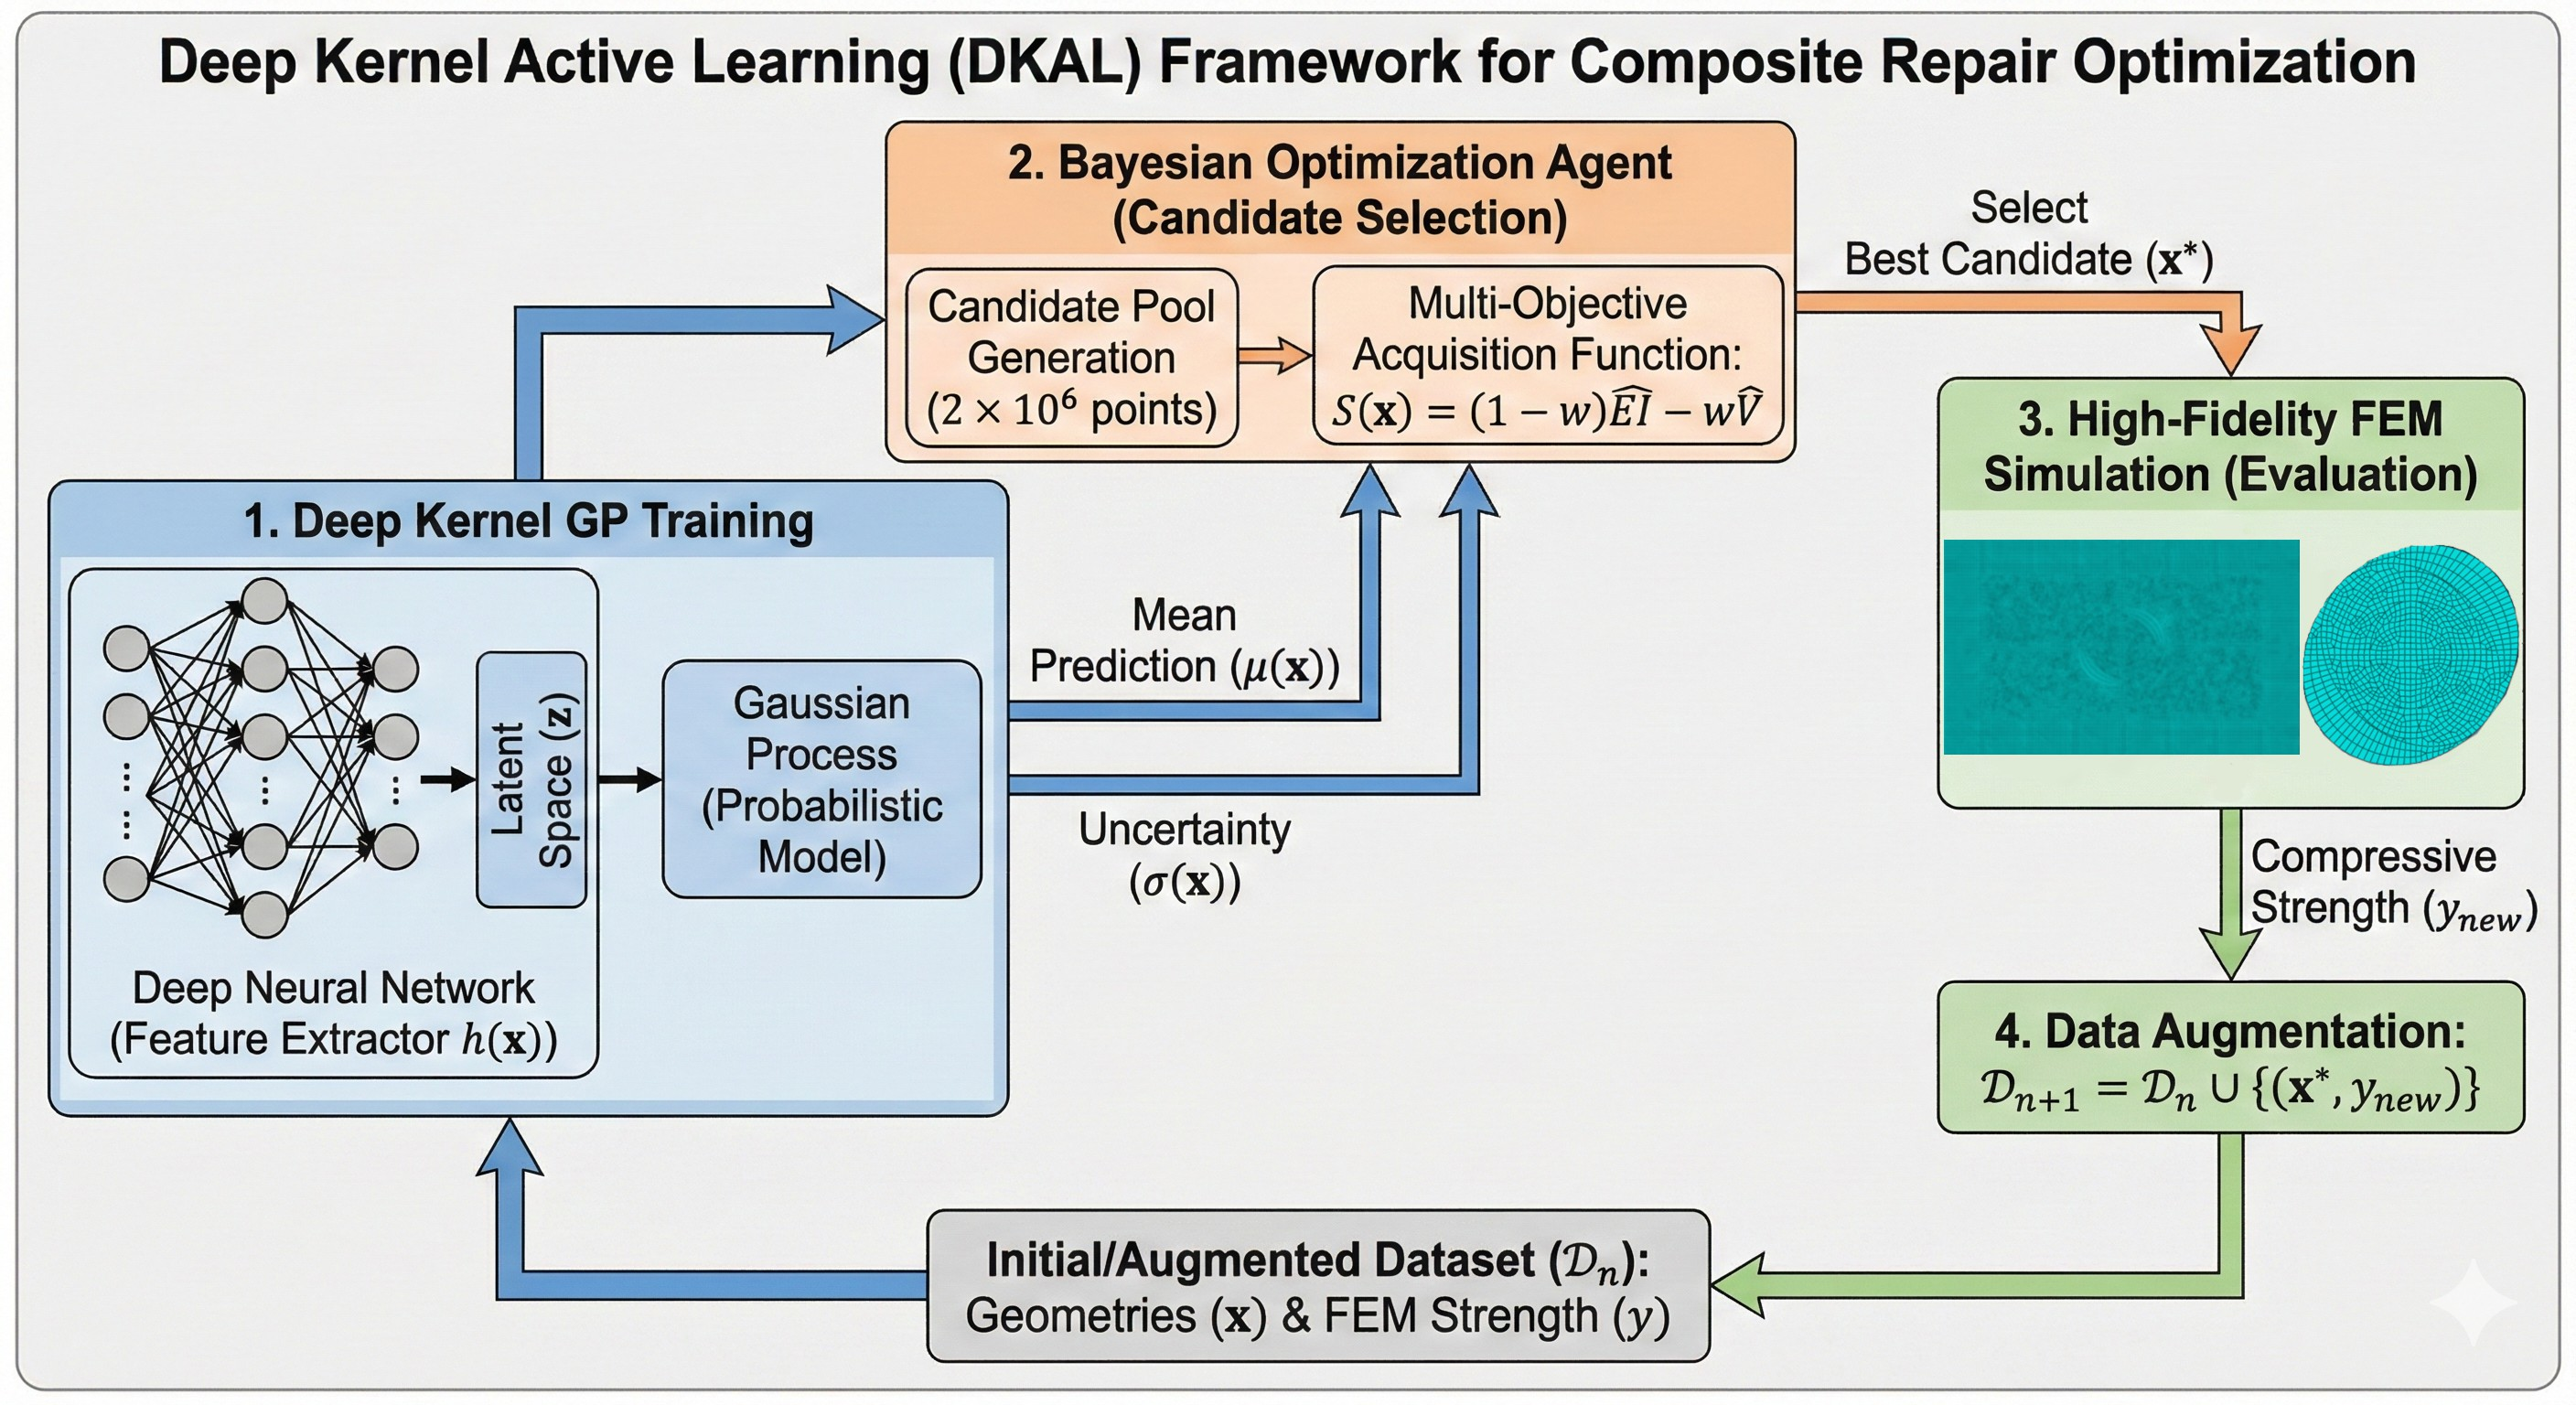
\includegraphics[width=\linewidth]{Algorithm_Flow.jpg}


% ==============================================================================
% 1. INTRODUCTION
% ==============================================================================
\section{Introduction}
\label{sec:intro}

The increasing adoption of fiber-reinforced polymer (FRP) composites in primary naval and aeronautical structures has driven the demand for reliable, high-performance repair methodologies. Unlike metallic structures, where bolted patches are standard, composite laminates benefit significantly from bonded stepped or scarf repairs. These configurations restore the aerodynamic continuity of the surface and provide a smoother stress transfer path compared to mechanical fastening \cite{baker1984structural, rhead2020analysis}. However, the geometric design of a stepped repair involves a complex multi-objective trade-off: maximizing the strength recovery requires long overlap lengths, which in turn necessitates the removal of excessive volumes of pristine parent material, increasing cost and downtime \cite{psarras2024design, pierce2019modelling}.

The structural response of a laminate under compressive loading is governed by intricate failure mechanisms, including local buckling, adhesive decohesion, and fiber kinking. Consequently, analytical closed-form solutions are often over-conservative. High-fidelity Finite Element Method (FEM) simulations utilizing Cohesive Zone Modeling (CZM) can accurately predict these failure modes \cite{turon2007engineering, alfano2001finite}, but they are computationally prohibitive for iterative optimization. A single non-linear progressive damage simulation can take several hours to converge; performing a global optimization search with thousands of evaluations is therefore operationally infeasible.

This computational bottleneck creates a significant challenge for standard engineering optimization strategies. Recent reviews highlight the growing adoption of \new{advanced computational methods} for composite optimization \cite{chen2023intelligent}. Applications range from optimizing manufacturing parameters using fuzzy logic \cite{babu2021artificial} to accelerating stress analysis via multi-fidelity machine learning \cite{azeem2024machine}. More advanced deep reinforcement learning strategies have also been proposed for \new{the optimization of woven composite microstructures} \cite{hsu2025ai}. However, despite these advances, the design of repair geometries remains a complex "black-box" problem characterized by non-convex failure surfaces and expensive constraints. Standard derivative-free methods, such as Genetic Algorithms (GA) or Particle Swarm Optimization (PSO), are widely used in composite design but are inherently "data-hungry," typically requiring thousands of function evaluations to ensure convergence \cite{deb2002fast, queipo2005surrogate}. \new{Similarly, although static sampling techniques such as Latin Hypercube Sampling (LHS) offer robust space-filling properties \cite{mckay1979comparison}, they are non-adaptive by construction: the full sample set is fixed a priori, so a surrogate built on LHS data has no mechanism to redirect subsequent evaluations toward high-performance regions of the design space.} Given the cost of the high-fidelity FEM, these traditional approaches become computationally intractable.

To address this sample efficiency limitations, this study adopts a \textit{Bayesian Active Learning} strategy. Unlike heuristic methods, Bayesian Optimization utilizes a probabilistic surrogate model to rigorously balance \textit{exploration} (reducing model uncertainty) and \textit{exploitation} (maximizing objective performance) \cite{shahriari2015taking}. This approach has been theoretically and empirically proven to identify global optima with orders of magnitude fewer evaluations than evolutionary strategies, making it the ideal candidate for data-sparse, computationally intensive engineering workflows \cite{jones1998efficient, ghosh2023digital}.

However, the success of Bayesian Optimization relies entirely on the quality of the underlying surrogate model, and standard architectures face significant limitations when applied to this domain. Standard \new{feed-forward neural networks} (NNs) are universal approximators but are inherently deterministic; they lack the intrinsic uncertainty quantification required to guide an \new{active-learning loop}. While techniques such as Monte Carlo (MC) Dropout \cite{gal2016dropout} or Deep Ensembles \cite{lakshminarayanan2017simple} can estimate uncertainty, they introduce distinct drawbacks. Deep Ensembles require training multiple models, multiplying the computational burden, while MC Dropout serves as a variational approximation that may not always provide robust uncertainty estimates in sparse data regimes.


Conversely, Gaussian Processes (GPs) provide a principled Bayesian framework, offering exact mean predictions and variance estimates \cite{rasmussen2006gaussian}. Yet, standard GPs struggle with both the "curse of dimensionality" and the complexity of the physical response. In a high-dimensional design space ($D=12$), standard stationary kernels (e.g., Radial Basis Function) rely on Euclidean distance metrics that fail to capture the underlying physics. Moreover, these kernels typically \new{impose a strong smoothness assumption that} is ill-suited for modeling sharp, non-linear bifurcations—such as the sudden onset of interfacial decohesion observed in stepped repairs. Without a powerful non-linear feature extractor to disentangle these complex interactions, standard GPs tend to over-smooth the objective landscape, thereby failing to resolve the critical "cliffs" in the failure surface.

To overcome these conflicting limitations—the lack of uncertainty in NNs and the lack of scalability in GPs—we propose a \textbf{Deep Kernel Gaussian Process (DKGP)} framework \cite{wilson2016deep}. This hybrid architecture utilizes a \new{deep neural network (DNN)} as a non-linear feature extractor, projecting the high-dimensional geometric inputs into a low-dimensional latent manifold. The Gaussian Process then operates on these expressive latent features. Effectively, the \new{DNN} learns an optimal kernel metric for the data, bypassing the need for manual kernel engineering while retaining the robust epistemic uncertainty quantification of the GP. \new{The resulting posterior variance} is critical for guiding the \new{Bayesian active learning loop} to efficiently navigate the sparse feasible region of the repair design space.

In a preceding study, Psarras et al. \cite{psarras2024design} established a parametric optimization framework based on analytical design heuristics. That approach relied on explicit physical laws—such as the stress intensity factor and adhesive shear strength—to generate candidate stepped geometries. While successful in identifying designs superior to standard circular patches, that methodology was inherently constrained by the simplifying assumptions of the analytical rules. The present work signifies a paradigm shift to a purely data-driven strategy. By treating the repair mechanics as a "black box" optimized by a \new{Deep Kernel surrogate}, we allow for the discovery of optimal configurations without pre-imposed constraints, enabling the identification of latent strengthening mechanisms that classical closed-form solutions fail to capture.

The remainder of this article is organized as follows. Section \ref{sec:methodology} first details the design of the experimental baseline and the high-fidelity finite element modeling used to establish the ground truth data. Section \ref{sec:AI_framework} then presents the proposed data-driven framework, describing the Deep Kernel architecture and the Bayesian Active Learning strategy. Section \ref{sec:results} analyzes the results, focusing on the \new{convergence rate} and the discovered multi-objective trade-off curve, alongside a physical interpretation of the optimal geometries. Finally, Section \ref{sec:conclusion} summarizes the key findings and conclusions.


\section{Experimental and Numerical Framework}
\label{sec:methodology}
The optimization framework relies on a robust baseline of experimental manufacturing con- straints and high-fidelity numerical simulations. This section outlines the geometric parametriza- tion, the manufacturing context (where repair volume serves as a direct proxy for process time), and the Finite Element Method (FEM) strategy used to generate the training data for the active learning algorithm.

\subsection{Problem Definition and Geometric Parametrization}

This study focuses on the repair of Carbon Fiber Reinforced Polymer (CFRP) laminates using a stepped patch repair technique \cite{psarras2024design}. The investigation considers a parent laminate plate with a stacking sequence of $[45^\circ/-45^\circ/90^\circ/0^\circ/90^\circ/0^\circ/90^\circ/-45^\circ/45^\circ]$. An initial damage depth of \new{$\approx 1.1$\,mm (six plies of $0.186$\,mm cured prepreg thickness)} is assumed, extending through the upper six plies \new{(``upper'' denotes the impact / loading-side surface; see Figure~\ref{fig:section21_schematic}(a) for a side cross-section)}. Consequently, the repair patch is designed to match the layup of the removed material: $[0^\circ/90^\circ/0^\circ/90^\circ/-45^\circ/45^\circ]$. Both the parent plate and the repair patch are modeled using \new{Cytec/Solvay CYCOM 977-2 unidirectional toughened-epoxy prepreg with IMS 24K carbon-fibre reinforcement}.

The experimental baseline assumes the use of a high-precision automated repair cell, where material removal and surface preparation are performed using a 20W pulsed green fiber laser (532 nm). The specific ablation parameters (pulse duration 1.5 ns, repetition rate 600 kHz) were selected based on previous statistical optimization studies by the authors \cite{psarras2020evaluating}, which demonstrated that such laser treatment significantly enhances adhesion properties. In this context, the minimization of the repair volume is not merely a material-saving objective but a critical \new{process-time} metric. Since the laser ablation process is volumetric in nature, minimizing the excavated material ($V$) is directly correlated with minimizing the total repair time ($t_{process} \propto V$). Therefore, the optimization algorithm aims to maximize strength while simultaneously minimizing the laser processing time.

\new{The repair geometry is parameterized into a design vector $\mathbf{x}$.} The repair consists of a parent structure with a stepped excavation and a matching patch, where the geometry is defined by the semi-axes of the elliptical steps. For a repair with $N=6$ \new{patch plies}, the design vector is defined as:
\begin{equation}
    \mathbf{x} = [a_1, a_2, \dots, a_6, b_1, b_2, \dots, b_6]
\end{equation}
where $a_i$ and $b_i$ represent the major and minor axes of the $i$-th \new{patch ply}, respectively.

\new{Two patch categories are considered. \textbf{Category 0 (aligned-orientation patches)} keeps all six elliptical steps oriented along the patch longitudinal axis. \textbf{Category 1 (mixed-orientation patches)} rotates each step by the orientation angle of the corresponding patch ply $[0^\circ/90^\circ/0^\circ/90^\circ/-45^\circ/45^\circ]$, so step contours follow the underlying fibre direction; this introduces the additional nesting constraint of Eq.~(4).}

To ensure physical manufacturability and geometric consistency, the optimization is subject to three sets of hard constraints \cite{psarras2024design}:

\begin{enumerate}
    \item \textbf{Domain Bounds:} All geometric parameters must lie within the feasible manufacturing window defined by the tool size and specimen dimensions:
    \begin{equation}
        L_{min} \leq a_i, b_i \leq L_{max}
    \end{equation}
    where $L_{min}=5$ mm and $L_{max}=35$ mm.

    \item \textbf{Hierarchical Nesting} (Category 0 \new{--- aligned-orientation patches}): For patches with aligned orientations (Category 0), ensuring a positive overlap is straightforward. Each subsequent \new{patch ply} must be strictly larger than the one beneath it:
    \begin{equation}
        a_i < a_{i+1} \quad \text{and} \quad b_i < b_{i+1}
    \end{equation}

    \item \textbf{\new{Scarfing Constraint}} (Category 1 \new{--- mixed-orientation patches}): For repairs involving varying \new{patch ply} orientations (e.g., $0^\circ/90^\circ$ interfaces), a stricter constraint is imposed \new{by the geometry of the laser scarfing process}. Since the removal process is sequential \new{--- the patch cavity is scarfed by the laser proceeding top-down, from the outermost patch ply ($\text{ply}_6$, at the upper face) inward to the innermost patch ply ($\text{ply}_1$, at the parent interface), and the laser can only remove material it can physically reach from above} ---, the outer \new{patch ply} ($i+1$) must geometrically encompass the inner \new{patch ply} ($i$) even when rotated\new{; any inner patch ply that would extend past the outer patch ply's footprint in the same direction is geometrically infeasible, since the corresponding material was already removed when the outer patch ply was scarfed and the laser cannot return to deposit material it has already ablated}. To prevent the major axis of an inner \new{patch ply} from protruding beyond the minor axis of a rotated outer \new{patch ply}, we enforce:
    \begin{equation}
        a_i \leq b_{i+1} \quad \forall i \in [1, N-1]
    \end{equation}
    This ensures that every \new{patch ply lies within the lateral envelope already ablated above it, so no inner patch ply requires material that the laser cannot reach from above}. \new{Figure~\ref{fig:section21_schematic}(b) illustrates this constraint by contrasting a valid configuration ($a_i \leq b_{i+1}$, inner patch ply fully within the laser-accessible region) with a violating one ($a_i > b_{i+1}$, lateral region inaccessible to the laser at the rotated edges).}

    \item \textbf{Aspect Ratio Constraint:} The parameter $a_i$ is defined as the longitudinal semi-axis. Consequently, the transverse semi-axis $b_i$ is constrained such that:
    \begin{equation}
        b_i \leq a_i
    \end{equation}
\end{enumerate}

These constraints define the valid design space $\mathcal{X}$, \new{effectively confining the surrogate-driven search to physically realizable boundaries.}

\new{\begin{figure}[htbp]
    \centering
    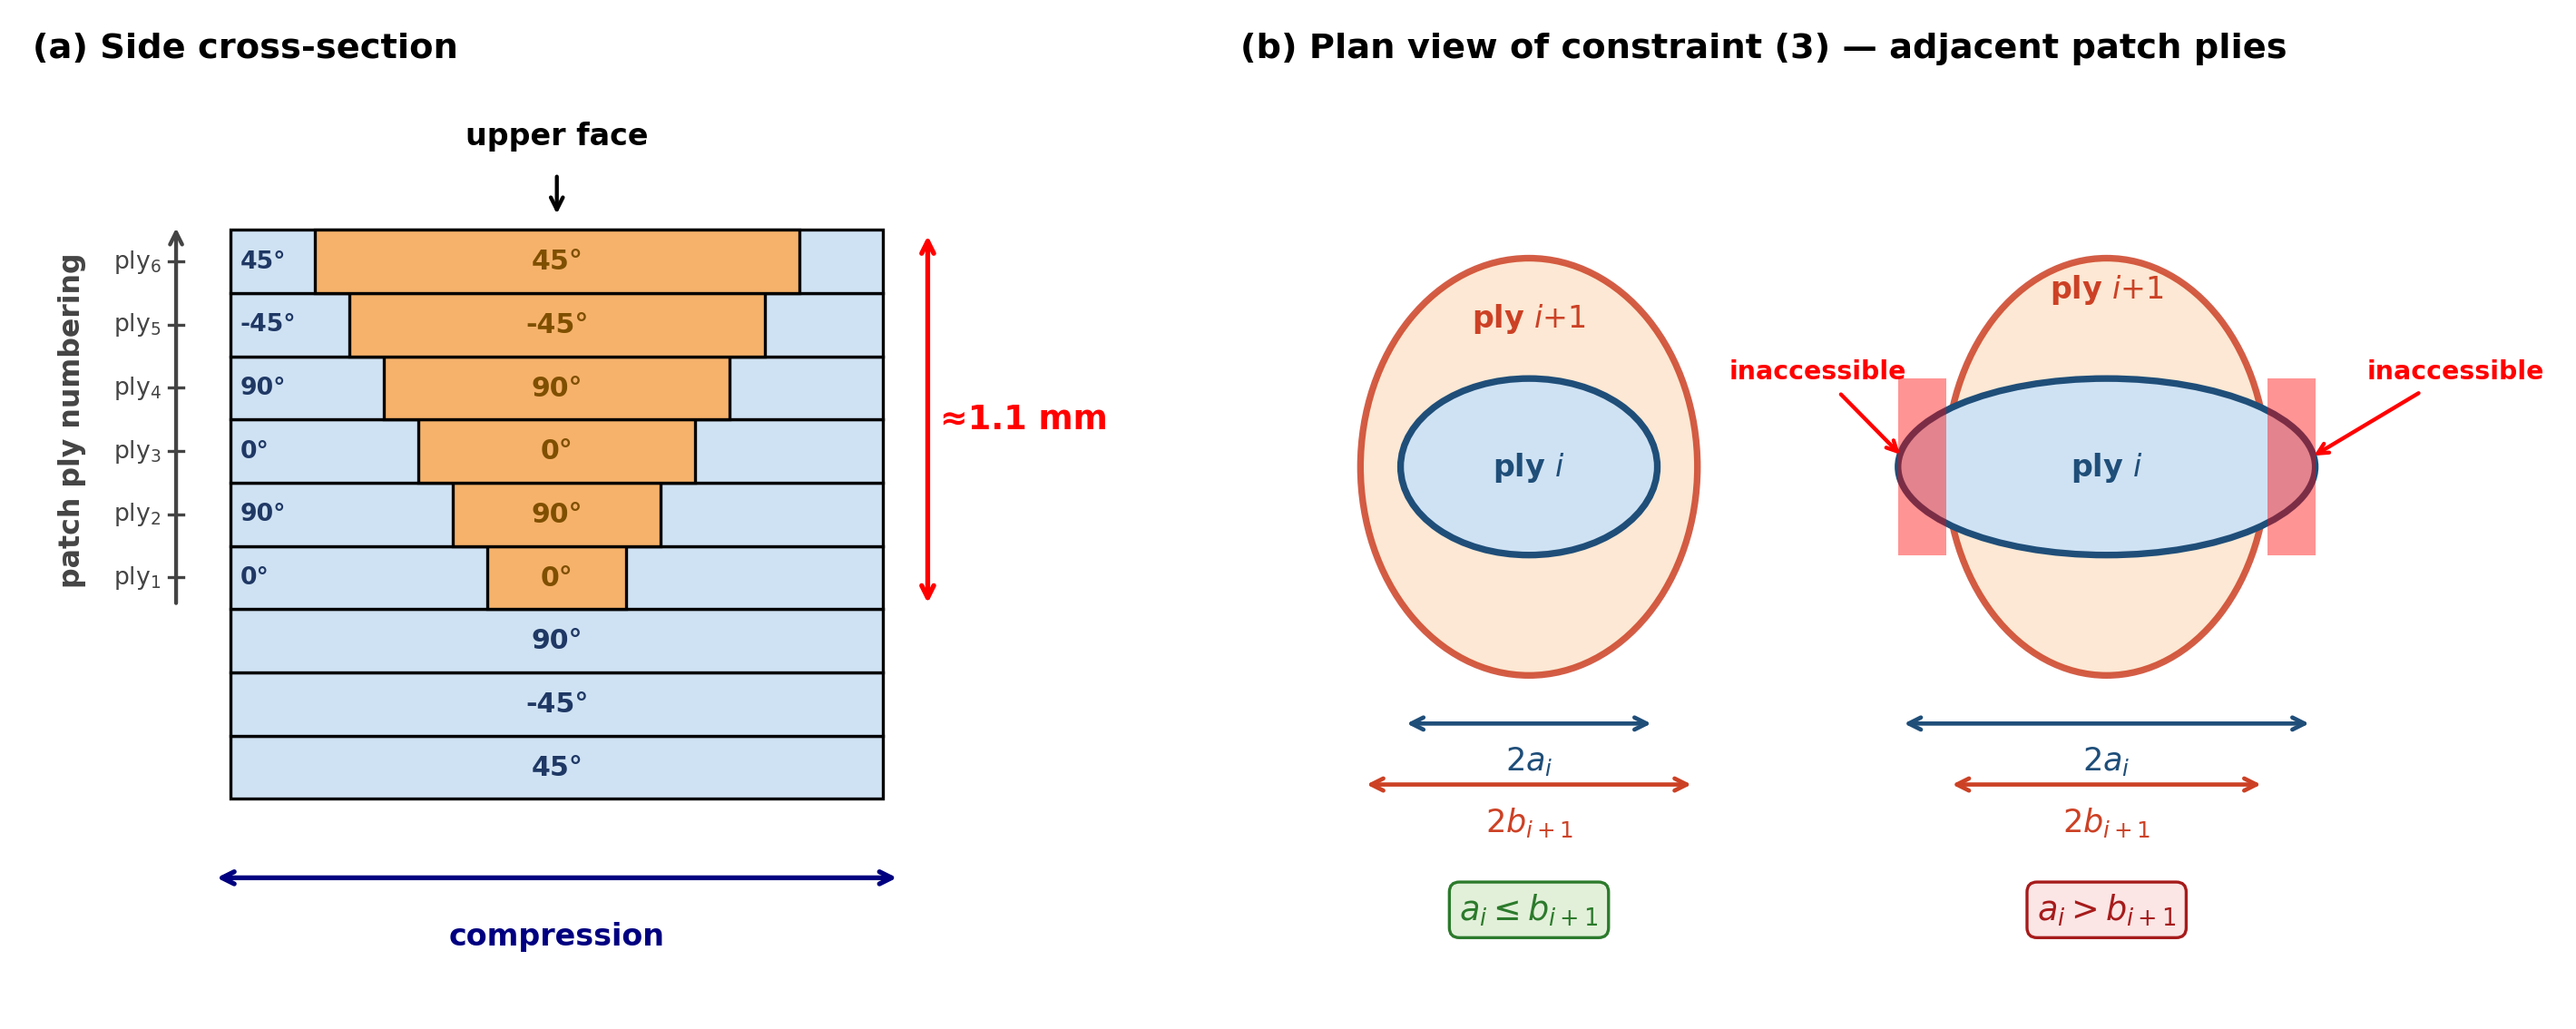
\includegraphics[width=\textwidth]{Section21_Schematic.png}
    \caption{Schematic of the stepped repair geometry and the Category~1 \new{scarfing constraint}. \textbf{(a)}~Side cross-section: the parent laminate (nine plies, layup $[45^{\circ}/-45^{\circ}/90^{\circ}/0^{\circ}/90^{\circ}/0^{\circ}/90^{\circ}/-45^{\circ}/45^{\circ}]$, read bottom-to-top) has its upper six plies excavated within an $\approx 1.1$\,mm damage depth (six plies $\times$ $0.186$\,mm cured prepreg) and replaced by a matching patch (orange steps) with layup $[0^{\circ}/90^{\circ}/0^{\circ}/90^{\circ}/-45^{\circ}/45^{\circ}]$. The upper face is the impact / loading-side surface; the lower three plies (light blue) remain intact across the full plate width. The left-side arrow indicates the patch ply numbering convention ($\text{ply}_1$ innermost, $\text{ply}_6$ outermost). The cohesive interface (zero-thickness COH3D8 elements) sits between each patch step and the underlying parent ply. \textbf{(b)}~Plan view of two consecutive patch plies in a Category~1 (mixed-orientation) repair. Constraint~(3) requires that the inner patch-ply major axis $a_i$ (blue) be no greater than the outer patch-ply minor axis $b_{i+1}$ in the same direction (red). The violating configuration on the right is included only to illustrate what the constraint excludes from the optimization search space; it is geometrically infeasible to manufacture, because the patch cavity is shaped by \new{laser scarfing} proceeding top-down from patch $\text{ply}_6$ (outermost) to patch $\text{ply}_1$ (innermost) --- once a patch ply's footprint has been cut, the lateral material at deeper levels is gone, and \new{any inner patch ply extending past the outer-ply footprint would lie in a region the laser cannot reach from above}.}
    \label{fig:section21_schematic}
\end{figure}}


\subsection{Finite Element Modelling Strategy}
Numerical simulations were performed using Abaqus/CAE 2024 to predict the Ultimate Compressive Strength (UCS). The model configuration is a version of the experimental setup specified by Airbus Standard AITM1-0010, aimed at assessing the compressive strength of a laminate plate post-impact (Compression After Impact), Figure \ref{fig:fea_setup}. The plate is affixed using two hard clamps, one on each lateral surface. One of the two clamps has all its degrees of freedom limited and displacement is applied on the other clamp. Also, in order to avoid buckling events, the model incorporates four anti-buckling semi-tubular rods on the bottom surface of the plate and four rods on the upper surface of the plate. \new{The parent laminate and the repair patch were modeled with 8-node continuum shell elements with reduced integration (SC8R), discretised explicitly through the thickness. The patch (layup $[0^\circ/90^\circ/0^\circ/90^\circ/-45^\circ/45^\circ]$) was modeled with one SC8R element per ply (six elements). The parent (layup $[45^\circ/-45^\circ/90^\circ/0^\circ/90^\circ/0^\circ/90^\circ/-45^\circ/45^\circ]$) was modeled with one SC8R element per ply for the upper six plies --- i.e.\ the plies that lie in the repair zone --- and a single sub-laminate element grouping the lower three plies, which remain intact below the damage depth (seven elements total). The adhesive layer was modeled with zero-thickness cohesive elements (COH3D8) inserted between the parent and patch steps.} A mesh sensitivity analysis was conducted to ensure numerical convergence. The mesh was locally refined in the scarf region to ensure that the characteristic cohesive zone length, Lcz, was spanned by at least 3-5 elements. This refinement is essential to prevent numerical instabilities and "snap-back" behavior during the propagation of adhesive damage \cite{turon2007engineering}.



\begin{figure}[htbp]
    \centering
    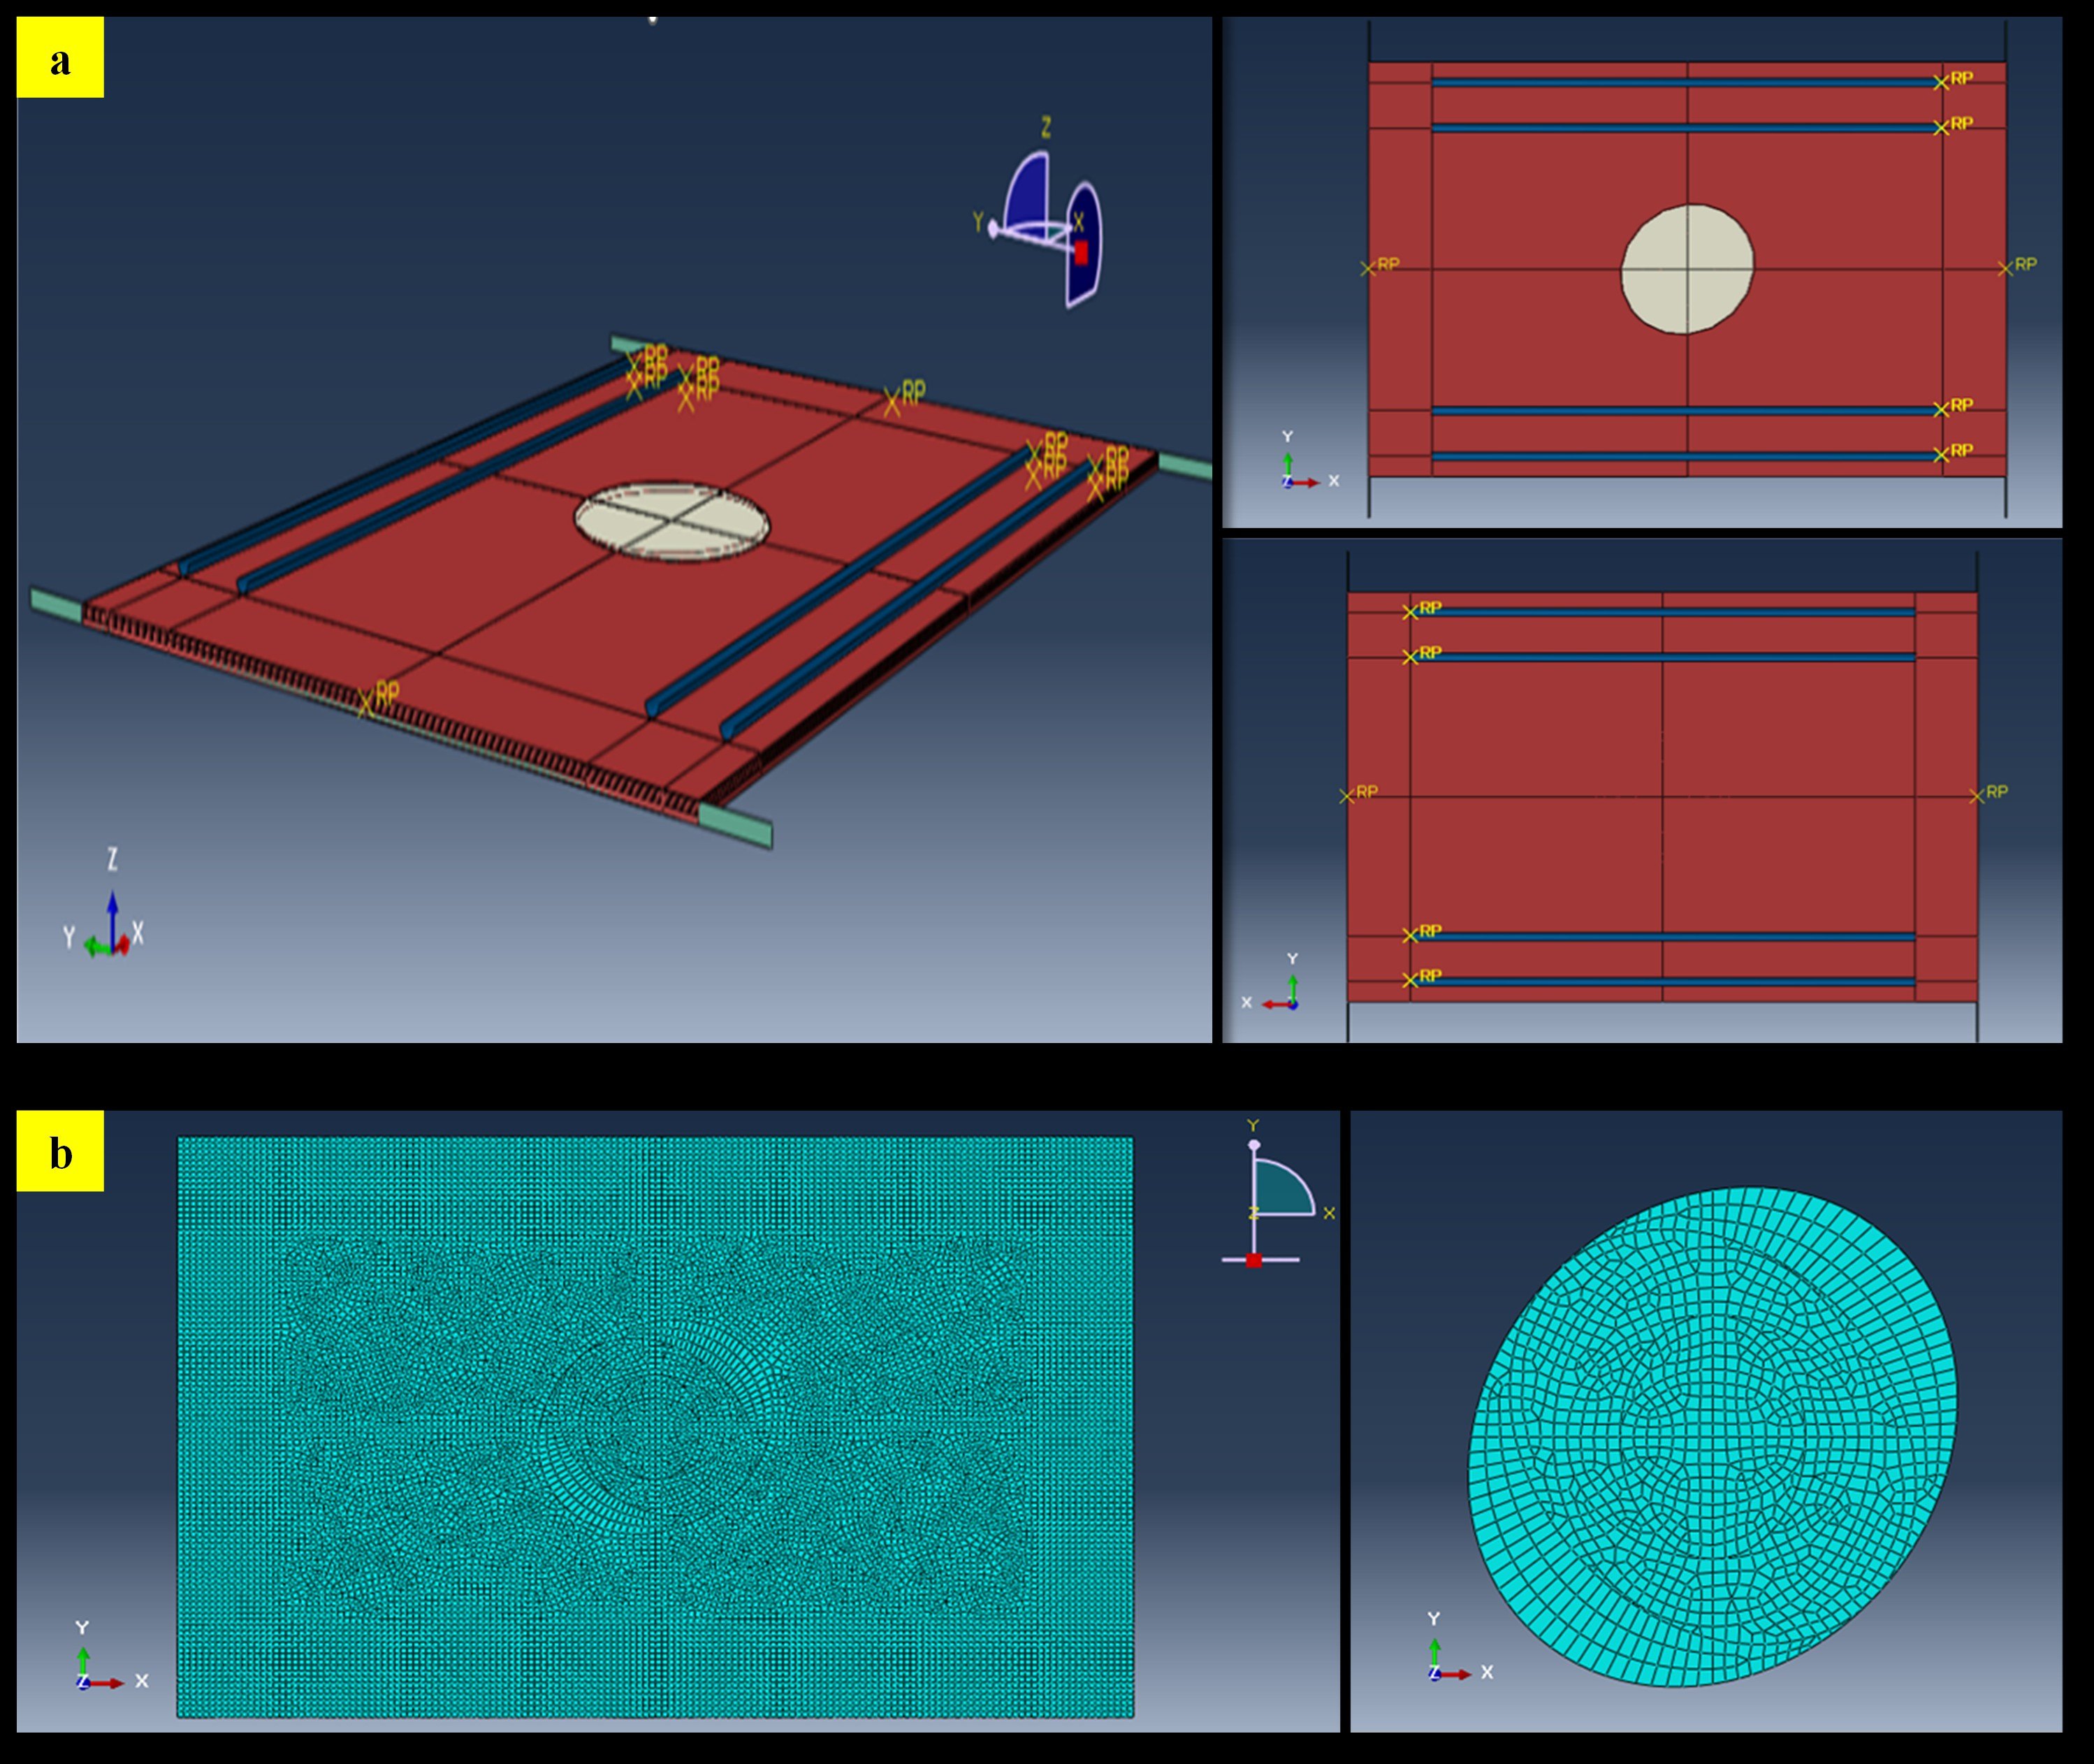
\includegraphics[width=0.9\linewidth]{FEA_Boundary_Conditions.jpg}
    \caption{Illustration of the Finite Element model configuration based on the Airbus AITM1-0010 standard for compression after impact showing (a) the clamping boundary conditions and the anti-buckling guide rods and (b) the mesh density of the plate and the patch.}
    \label{fig:fea_setup}
\end{figure}



To predict failure within the composite plies, the Hashin failure criteria were implemented \cite{hashin1980failure}, monitoring fiber and matrix failure modes under compression and tension. The specific material properties used for the composite material and the adhesion are detailed in Table \ref{tab:material_properties}. This specific FE methodology, including the sub-laminate approach and cohesive zone definition, has been extensively validated by the authors against experimental compression tests \cite{psarras2020evaluating, psarras2023evaluating}, demonstrating high fidelity in predicting both the failure modes and the ultimate failure loads. \new{Rather than a stand-alone mesh-refinement convergence study, the present methodology --- including the SC8R element type, the local mesh refinement at the step corners (at least 3--5 elements spanning the cohesive zone length $L_{cz}$), and the calibrated material card of Table~\ref{tab:material_properties} --- has been validated end-to-end against experimental compression-after-impact data at the coupon and subcomponent scales \cite{psarras2024design, psarras2020evaluating, psarras2023evaluating}. The $\approx 95\,\%$ strength-recovery limit reported in Section~\ref{sec:results} therefore reflects an experimentally anchored physical saturation.}

\begin{table}[htbp]
    \centering
    \caption{Calibrated Material Properties for the FE Model.}
    \label{tab:material_properties}
    \renewcommand{\arraystretch}{1.2}
    \begin{tabular}{l l r}
        \toprule
        \textbf{Parameter} & \textbf{Symbol} & \textbf{Value} \\
        \midrule
        \multicolumn{3}{c}{\textbf{Composite Lamina}} \\
        \textit{\textbf{Elastic Properties}} & & \\
        Density & $\rho$ & $1.597 \times 10^{-6}$ kg/mm$^3$ \\
        Longitudinal Modulus & $E_{11}$ & 125.0 GPa \\
        Transverse Modulus & $E_{22}$ & 8.68 GPa \\
        Shear Modulus & $G_{12}$ & 4.70 GPa \\
        Poisson's Ratio & $\nu_{12}$ & 0.35 \\
        
        \textit{\textbf{Strengths}} & & \\
        Fiber Tensile Strength & $X_T$ & 3325 MPa \\
        Fiber Compressive Strength & $X_C$ & 911 MPa \\
        Matrix Tensile Strength & $Y_T$ & 66 MPa \\
        Matrix Compressive Strength & $Y_C$ & 170 MPa \\
        In-Plane Shear Strength & $S_{12}$ & 90 MPa \\
        Interlaminar Shear Strength & $S_{23}$ & 60 MPa \\
        
        \textit{\textbf{Fracture Energies}} & & \\
        Fiber Tension & $G_{ft}$ & 163 N/mm \\
        Fiber Compression & $G_{fc}$ & 70 N/mm \\
        Matrix Tension & $G_{mt}$ & 0.5 N/mm \\
        Matrix Compression & $G_{mc}$ & 17 N/mm \\
        
        \midrule
        \multicolumn{3}{c}{\textbf{Cohesive}} \\
        \textit{\textbf{Elastic Stiffnesses}} & & \\
        Normal Stiffness & $K_{nn}$ & \new{100 kN/mm$^3$} \\
        Shear Stiffness & $K_{ss}, K_{tt}$ & \new{35 kN/mm$^3$} \\
        
        \textit{\textbf{Damage Initiation}} & & \\
        Normal Strength & $t_n^0$ & 14 MPa \\
        Shear Strength & $t_s^0, t_t^0$ & 40 MPa \\
        
        \textit{\textbf{Damage Evolution}} & & \\
        Critical Fracture Energy (Normal) & $G_{Ic}$ & \new{0.4 N/mm} \\
        Critical Fracture Energy (Shear) & $G_{IIc}$ & \new{0.6 N/mm} \\
        \bottomrule
    \end{tabular}
\end{table}

% ==============================================================================
% 3. DEEP KERNEL ACTIVE LEARNING
% ==============================================================================
\section{Deep Kernel Active Learning Framework}
\label{sec:AI_framework}

To overcome the computational cost of high-fidelity FEM simulations, this study proposes a probabilistic active learning framework. Unlike traditional surrogate modeling approaches that rely on static datasets—such as Response Surface Methodology (RSM) or standard Neural Networks \cite{queipo2005surrogate, luo2020surrogate}—we employ a Deep Kernel Gaussian Process (DKGP) \cite{wilson2016deep}. This architecture combines the feature-learning capabilities of deep neural networks with the uncertainty quantification of Gaussian Processes, enabling a query-based optimization strategy that specifically targets high-value and high-uncertainty regions of the design space \cite{ghosh2023digital}.

\new{Figure~\ref{fig:algorithm_flow} provides a high-level overview of the framework and shows how the components introduced in this section link together. The four numbered blocks correspond, in turn, to the Deep Kernel GP and its kernel choice (Block~1, Sections~3.1--3.3), the \new{Bayesian acquisition step that scores} candidate designs (Block~2, Section~3.4), the high-fidelity FEM evaluation that returns the measured compressive strength (Block~3, Section~2.2), and the data-augmentation step that re-enters Block~1 to retrain the surrogate (Block~4, Section~3.5).}

\begin{figure}[htbp]
    \centering
    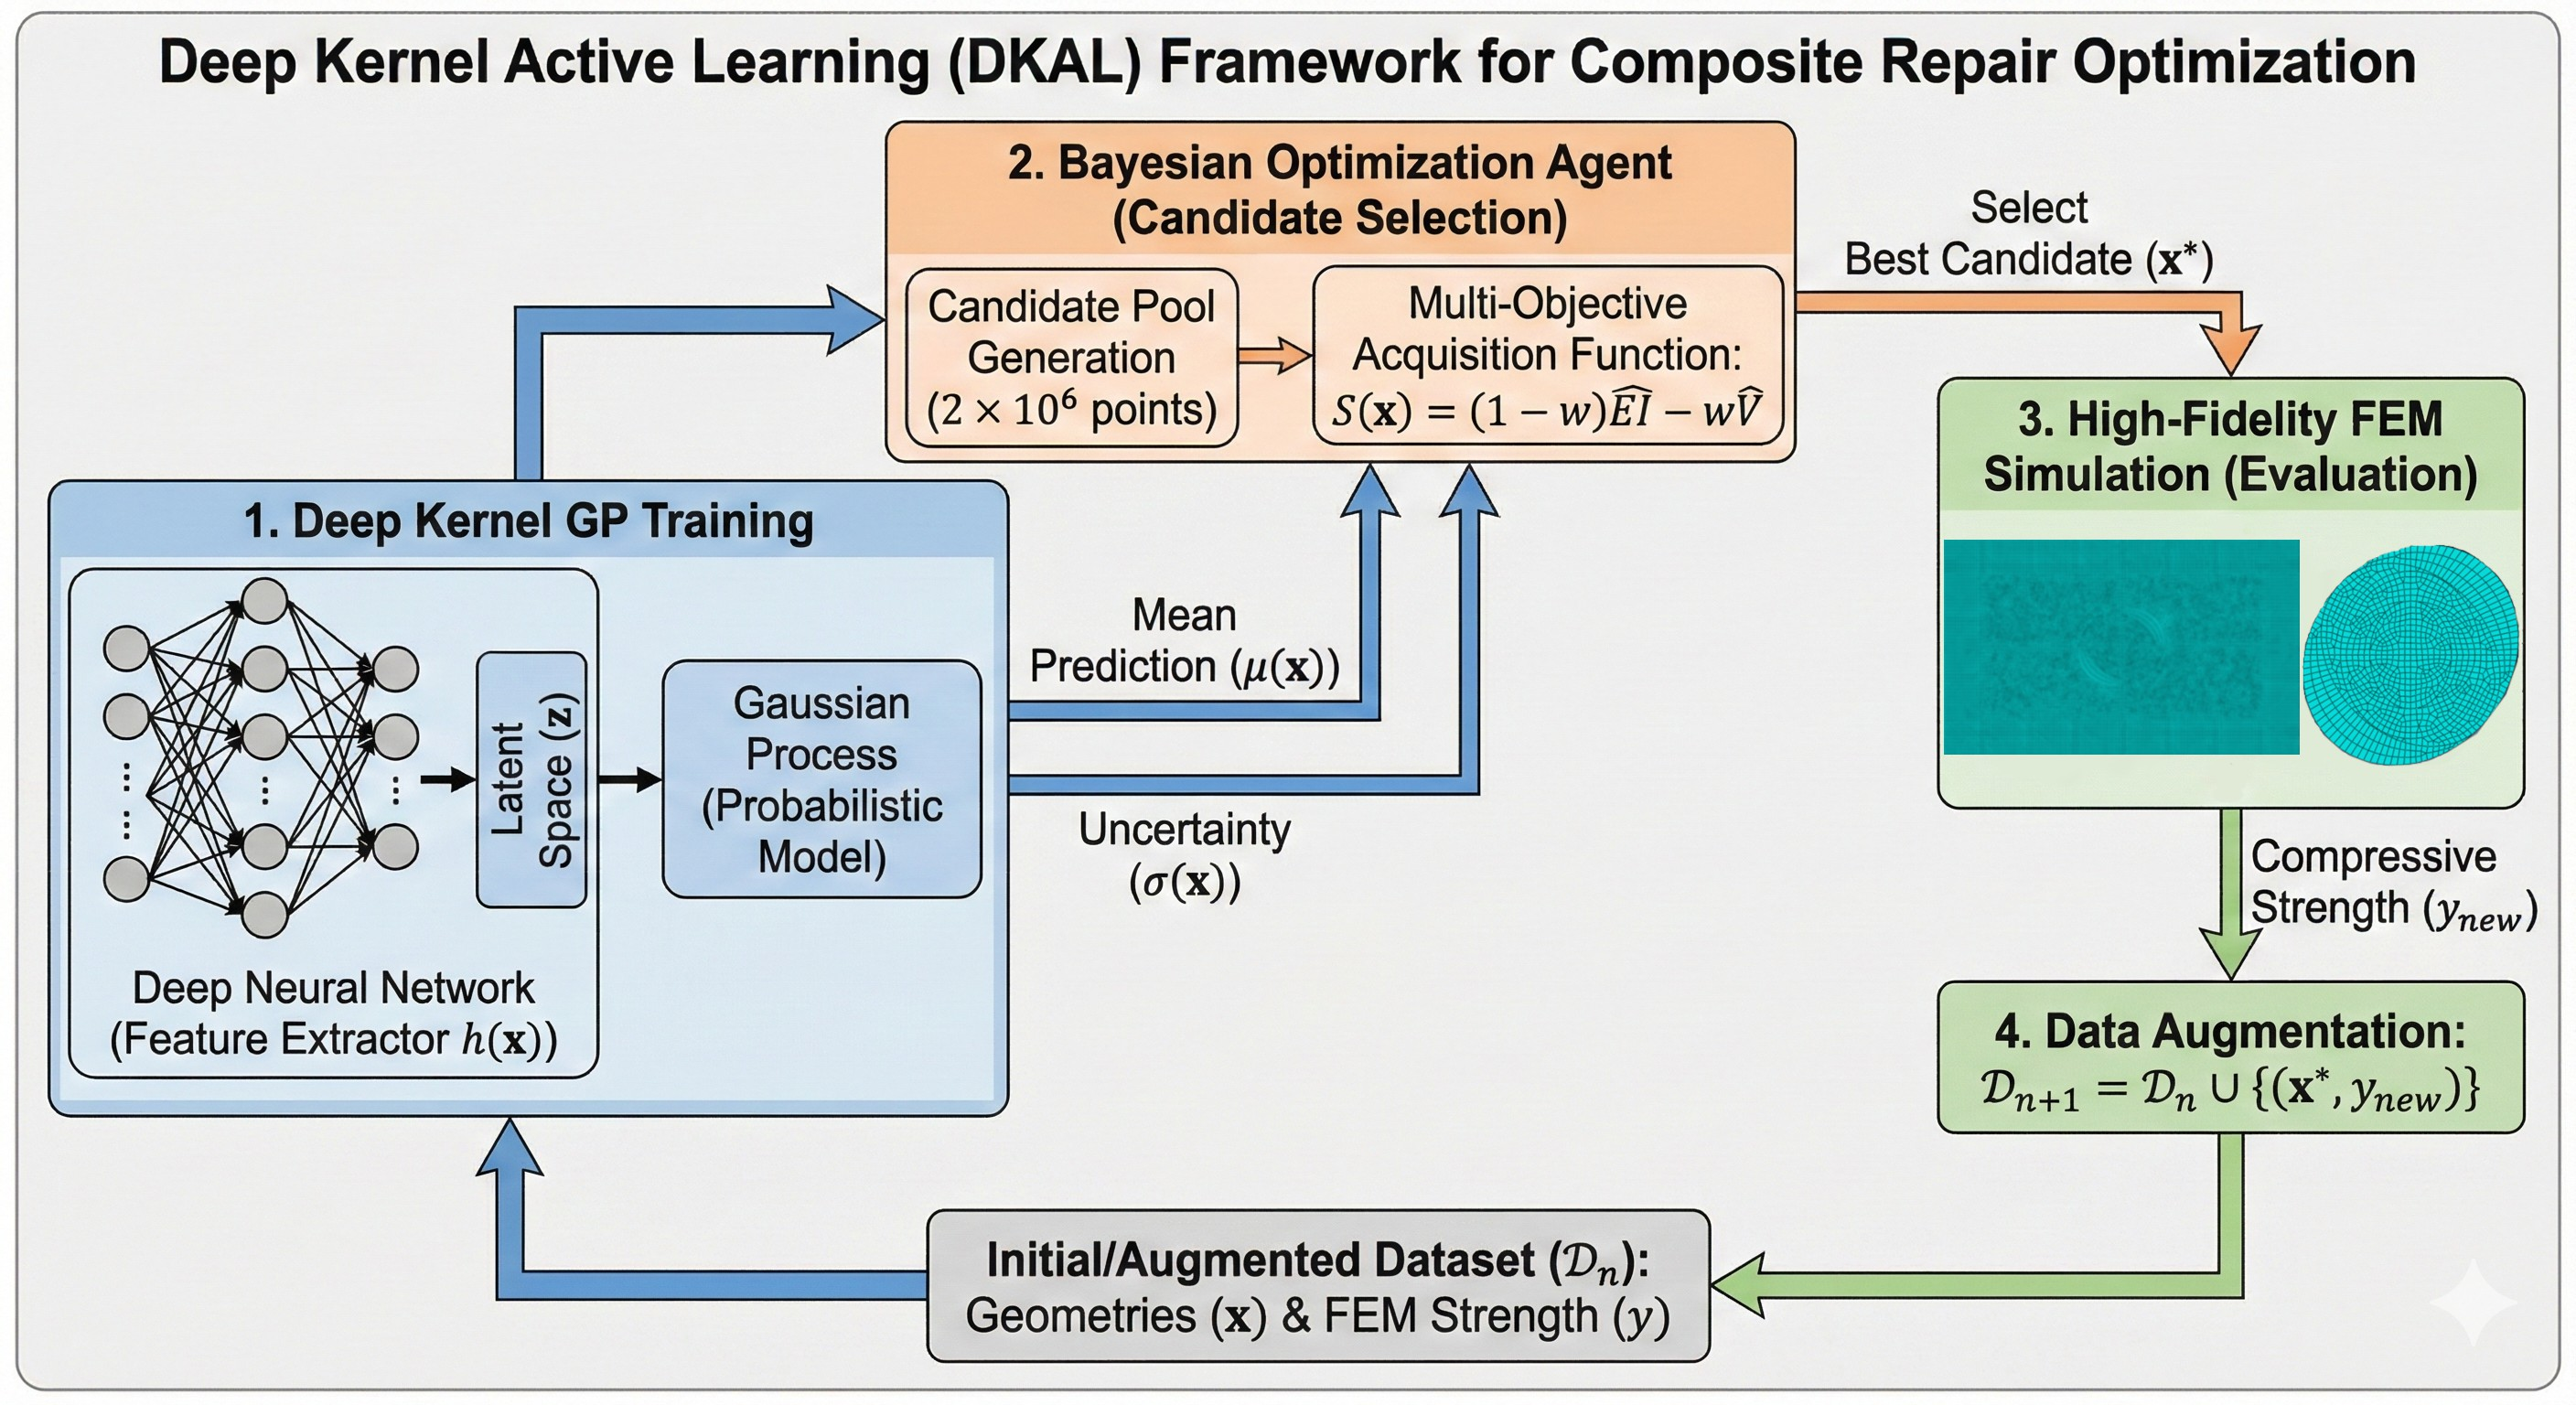
\includegraphics[width=\textwidth]{Algorithm_Flow.jpg}
    \caption{Schematic of the Deep Kernel Active Learning (DKAL) framework. The closed-loop process iterates between four blocks. \new{\textbf{(1) Deep Kernel GP training} (Sections~3.1--3.3): a DNN feature extractor $h(\mathbf{x};\mathbf{w})$ projects the design vector into a latent space $\mathbf{z}$, which is then fed to a Gaussian Process to produce a mean prediction $\mu(\mathbf{x})$ and an uncertainty $\sigma(\mathbf{x})$. \textbf{(2) \new{Bayesian acquisition step}} (Section~3.4): a Monte Carlo candidate pool is scored by the multi-objective acquisition function $S(\mathbf{x})$. \textbf{(3) High-fidelity FEM simulation} (Section~2.2): the selected design $\mathbf{x}^{*}$ is evaluated with the Abaqus model, returning the measured compressive strength $y_{\text{new}}$. \textbf{(4) Data augmentation} (Section~3.5): the new pair $(\mathbf{x}^{*}, y_{\text{new}})$ is appended to the dataset, $\mathcal{D}_{n+1} = \mathcal{D}_n \cup \{(\mathbf{x}^{*}, y_{\text{new}})\}$, and the loop returns to Block~1 to retrain the surrogate.}}
    \label{fig:algorithm_flow}
\end{figure}

\subsection{Deep Kernel Gaussian Process (DKGP) Formulation}
\new{To address the curse-of-dimensionality limitation of standard Gaussian Processes (Section~\ref{sec:intro})}, we utilize a Deep Kernel Learning (DKL) approach. The model consists of two coupled components: a Deep Neural Network (DNN) feature extractor $h(\mathbf{x}; \mathbf{w})$ and a Gaussian Process layer. \new{The parameter set $\mathbf{w} = \{\mathbf{W}_l, \mathbf{b}_l\}_{l=1}^{L}$ collects the $L$ weight matrices and bias vectors of the DNN and is learned jointly with the GP hyperparameters.}

Let $\mathbf{x} \in \mathbb{R}^{12}$ be the input design vector representing the \new{patch ply} definitions (6 lengths $a_i$ and 6 widths $b_i$). The feature extractor projects this high-dimensional input into a compressed, lower-dimensional latent manifold $\mathbf{z} \in \mathbb{R}^3$:
\begin{equation}
    \mathbf{z} = h(\mathbf{x}\new{; \mathbf{w}}) = \phi\!\left(\mathbf{W}_L\,\phi\!\left(\mathbf{W}_{L-1}\,\dots\,\phi(\mathbf{W}_1 \mathbf{x} + \mathbf{b}_1)\,\dots + \mathbf{b}_{L-1}\right) + \mathbf{b}_L\right)
\end{equation}
\new{where $\phi(\cdot)$ denotes the element-wise Gaussian Error Linear Unit (GELU) activation.} The Gaussian Process is then defined over these latent features $\mathbf{z}$ rather than the raw inputs $\mathbf{x}$.

\subsection{Two-Stage Adaptive Strategy}
\label{sec:two_stage}
To efficiently navigate the design space while mitigating the "cold start" problem (overfitting on sparse initial data), we employ a Progressive Complexity Strategy. The surrogate model architecture adapts as the dataset grows, transitioning from a robust exploration mode to a high-fidelity exploitation mode (Table \ref{tab:phases}).

\begin{table}[htbp]
    \centering
    \caption{Configuration of the Two-Stage Active Learning Strategy. The model complexity adapts from exploration (Phase I) to exploitation (Phase II).}
    \label{tab:phases}
    \begin{tabular}{l l l}
        \toprule
        \textbf{Component} & \textbf{Phase I (Exploration)} & \textbf{Phase II (Refinement)} \\
        \midrule
        \textbf{Objective} & Discover promising regions & Pinpoint global optimum \\
        \textbf{Network Depth} & Shallow MLP (2 Layers) & Deep Compressive ResNet (6 Layers) \\
        \textbf{Kernel Prior} & RBF (Smooth, $C^\infty$) & Matern 5/2 (Rough, $C^2$) \\
        \textbf{Data Regime} & Sparse ($N < 70$) & Dense ($N \geq 70$) \\
        \bottomrule
    \end{tabular}
\end{table}

\textbf{Phase I (Exploration):} In the initial stages, a shallow network is combined with a standard Radial Basis Function (RBF) kernel to enforce smoothness and prevent the model from hallucinating artifacts:
\begin{equation}
    k_{RBF}(\mathbf{z}, \mathbf{z}') = \sigma_f^2 \exp\left( - \frac{||\mathbf{z} - \mathbf{z}'||^2}{2\ell^2} \right)
\end{equation}
where \new{$\mathbf{z}, \mathbf{z}' \in \mathbb{R}^3$ are two latent feature vectors produced by the DNN (Eq.~(6)), $\sigma_f^2$ is the signal variance, and} $\ell$ is a global length-scale parameter.

\textbf{Phase II (Refinement):} As data density increases, the model transitions to the Deep architecture described in Section \ref{sec:architecture} and \new{replaces the RBF prior with a Matern 5/2 kernel}:
\begin{equation}
    k_{Mat}(\mathbf{z}, \mathbf{z}') = \sigma_f^2 \left( 1 + \sqrt{5}\,d + \frac{5}{3}\,d^2 \right) \exp\left(-\sqrt{5}\,d\right),
\end{equation}
\new{where $d = \|\mathbf{z}-\mathbf{z}'\|/\ell$ is the Euclidean distance in the latent space normalised by a single length-scale $\ell$, and $\mathbf{z}, \mathbf{z}' \in \mathbb{R}^3$ are the latent feature vectors of Eq.~(6). Although both the RBF and the Matern 5/2 priors yield smooth sample paths (with $C^{\infty}$ and $C^2$ continuity, respectively), the Matern 5/2 covariance decays more rapidly with distance: nearby latent points remain strongly coupled, while far-away points decouple faster than under the RBF prior. This shorter effective correlation range is better matched to the present problem, where the strength response varies rapidly --- but continuously --- around the onset of premature adhesive debonding (Section~\ref{sec:results}); the $C^{\infty}$ RBF prior would over-smooth these steep local gradients. Both isotropic and ARD variants of this kernel were tested during development; the isotropic form was retained as more parsimonious in the present low-data regime.}

\subsection{Network Architecture Implementation}
\label{sec:architecture}
For the final high-fidelity surrogate (Phase II), the architecture functions as a non-linear dimensionality reduction funnel. As shown in Figure \ref{fig:architecture}, it employs a Compressive Residual Network topology that linearly decreases in width from the input ($D_{in}=12$) to the latent manifold ($D_{out}=3$).



\begin{figure}[htbp]
    \centering
    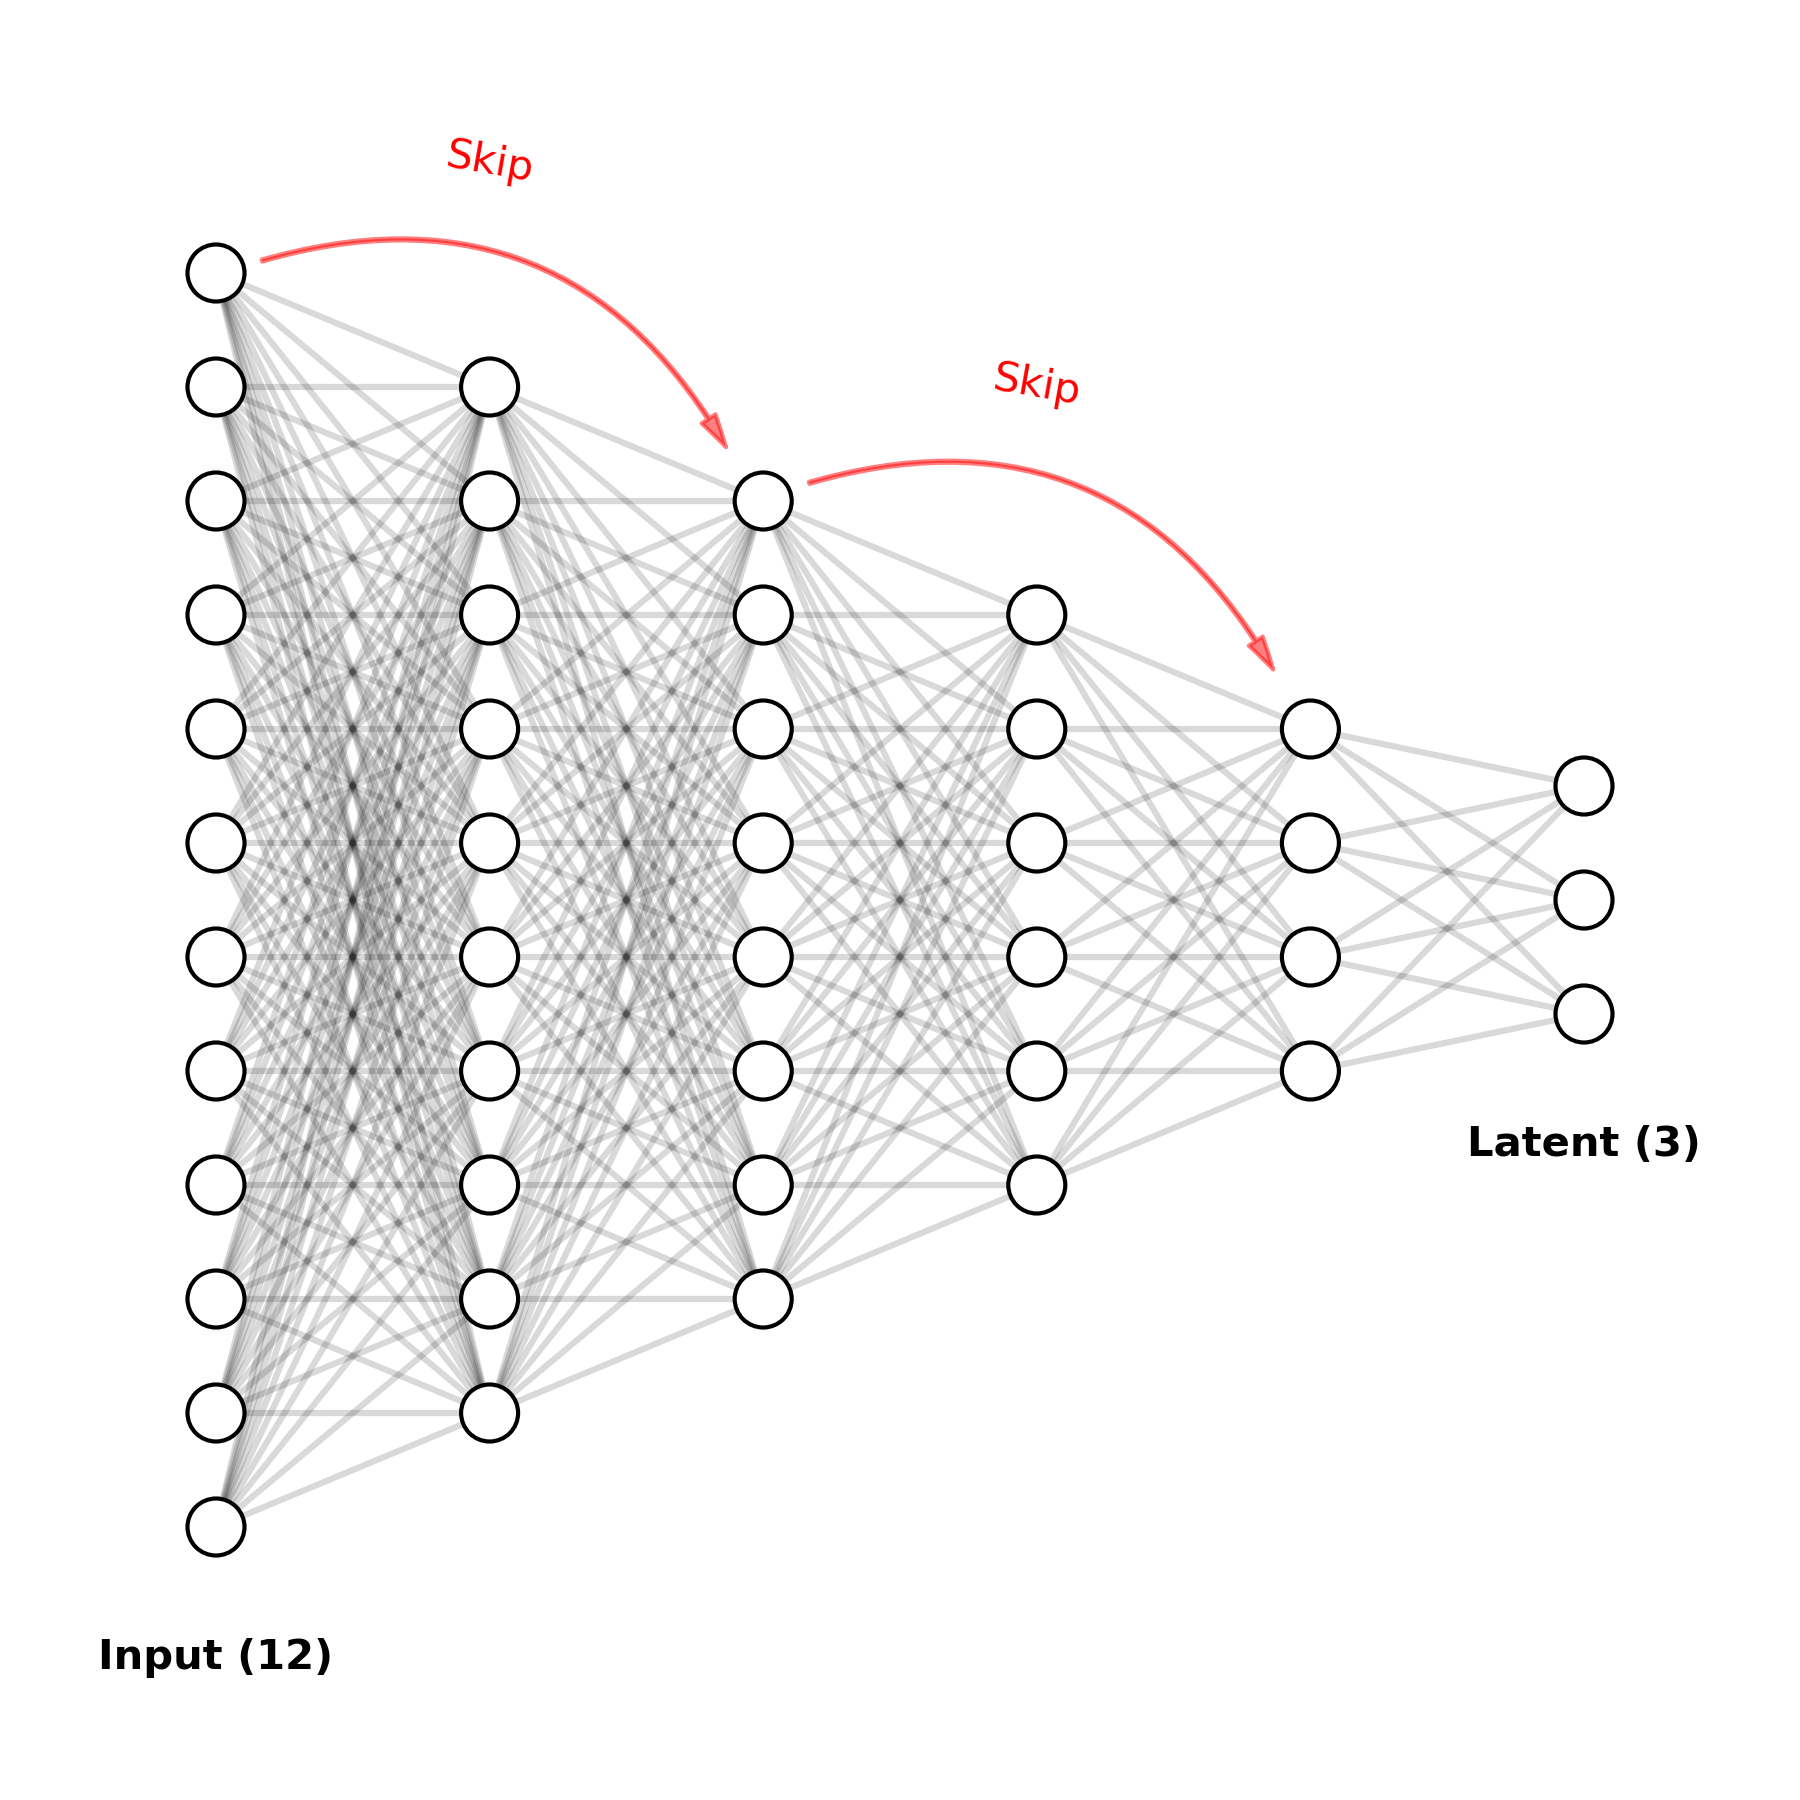
\includegraphics[width=0.7\linewidth]{model_architecture.png}
    \caption{The Deep Kernel architecture featuring a "Compressive Tower" topology. The network linearly decreases in width from the input dimension (12) to the latent dimension (3) over 6 layers. Residual skip connections (red) are utilized every 2 layers to preserve gradient flow during the compression.}
    \label{fig:architecture}
\end{figure}

The specific hyperparameters (Table \ref{tab:hyperparameters}) were selected to enforce regularization. Notably, residual skip connections are inserted every 2 layers to prevent vanishing gradients, preserving gradient flow \cite{he2016deep}, and a Dropout rate of $p=0.1$ is applied to simulate ensemble effects.

\begin{table}[htbp]
    \centering
    \caption{Hyperparameter configuration for the Deep Kernel Surrogate.}
    \label{tab:hyperparameters}
    \begin{tabular}{l l}
        \toprule
        \textbf{Parameter} & \textbf{Value/Setting} \\
        \midrule
        Input Dimension & 12 ($a_1\dots a_6, b_1\dots b_6$) \\
        Latent Dimension & 3 \\
        Network Depth & 6 Layers \\
        Hidden Widths & Linear Decay: $[12, 10, 8, 6, 4, 3]$ \\
        Activation Function & GELU (Gaussian Error Linear Unit) \\
        Skip Connections & Residual Block every 2 layers \\
        Dropout Rate & $p=0.1$ \\
        \midrule
        GP Kernel & \new{Matern $5/2$ (isotropic)} \\
        GP Likelihood & Gaussian (Homoscedastic) \\
        Optimizer & AdamW ($\lambda=1\times 10^{-4}$) \\
        Training Epochs & 10,000 \\
        \bottomrule
    \end{tabular}
\end{table}

\subsection{Multi-Objective Candidate Selection}
To minimize the number of expensive FEM calls, we implement a Bayesian Optimization loop using the Expected Improvement (EI) acquisition function \cite{jones1998efficient}. This strategy balances \textit{exploitation} (refining high-strength designs) and \textit{exploration} (investigating uncertain geometries).

The standard \new{Expected Improvement} acquisition function $\alpha(\mathbf{x})$ is computed as:
\begin{equation}
    \new{\alpha(\mathbf{x}) =} (\mu(\mathbf{x}) - y_{best}^+) \Phi(Z) + \sigma(\mathbf{x}) \phi(Z)
\end{equation}
where $Z = \frac{\mu(\mathbf{x}) - y_{best}^+}{\sigma(\mathbf{x})}$, $\mu(\mathbf{x})$ and $\sigma(\mathbf{x})$ are the predictive mean and standard deviation from the Deep Kernel GP, \new{$y_{best}^+ = \max_{i=1,\dots,N}\, y_i$ is the best objective value observed across the $N$ designs already evaluated,} and $\Phi$ and $\phi$ are the standard normal cumulative distribution and probability density functions, respectively.

However, the optimization problem is multi-objective: we seek to maximize compressive strength while strictly minimizing the repair volume. To embed this manufacturing constraint directly into the selection process, the final selection score $S(\mathbf{x})$ is defined as a weighted combination of the probabilistic improvement and the geometric cost:

\begin{equation}
    S(\mathbf{x}) = (1 - w) \cdot \widehat{EI}(\mathbf{x}) - w \cdot \widehat{V}(\mathbf{x})
\end{equation}

where $\widehat{EI}$ is the min-max normalized Expected Improvement (scaled to $[0,1]$), $\widehat{V}$ is the normalized volume of the repair patch, and $w$ is a weighting factor set to $0.5$ to balance structural performance and material usage equally. This ensures the optimizer prioritizes designs that offer high strength gains per unit of material added.

\subsection{Active Learning Procedure}
The active learning loop, illustrated in Figure \ref{fig:algorithm_flow}, proceeds as follows:

\begin{enumerate}
    \item \textbf{Initialization} (Warm Start): The loop is seeded with \new{high-fidelity evaluations from a previous parametric study \cite{psarras2024design}: 38 designs for Category 0 and 28 for Category 1,} providing a robust baseline of competent designs.
    \item \textbf{Adaptive Training:} The DKGP is retrained on the cumulative dataset. The architecture (Shallow vs. Deep) and Kernel (RBF vs. Matern) are automatically selected based on the dataset size, following the strategy defined in Section \ref{sec:two_stage}.
    \item \textbf{Candidate Search:} A Monte Carlo search of $2 \times 10^6$ valid integer points is performed. Constraints ensure \new{patch ply} dimensions are non-decreasing ($a_i \leq a_{i+1}$).
    \item \textbf{Update:} The candidate maximizing $S(\mathbf{x})$ is evaluated in FEM and appended to the dataset.
\end{enumerate}

\subsection{Implementation and Computational Resources}
\label{sec:implementation}

The active learning framework was \new{implemented in Python and automates the exchange of designs and responses between the surrogate and the finite element solver.} The Deep Kernel architecture was implemented using PyTorch \cite{paszke2019pytorch} and GPyTorch \cite{gardner2018gpytorch}, utilizing GPU acceleration. The Finite Element evaluations were executed using Abaqus/Standard 2024, interfaced via Abaqus-Python scripting.

All computations were performed on a dedicated workstation equipped with an AMD Ryzen 9-5900X processor (12 cores), 64 GB of RAM, and a NVIDIA RTX 3070 GPU. The computational cost breakdown per iteration is detailed below:

\begin{itemize}
    \item \textbf{Finite Element Simulation (Bottleneck):} The high-fidelity progressive damage analysis required approximately \textbf{3 to 4 hours} of wall-clock time per design evaluation, depending on the complexity of the damage propagation.
    \item \textbf{Surrogate Training and Query:} In contrast, the Deep Kernel retraining (10,000 epochs) and the candidate search over the $2 \times 10^6$ integer pool required \textbf{3 minutes} on the GPU per category.
\end{itemize}


\subsection{Rationale for Architectural Design}
\label{sec:ai_rationale}

The architecture was refined to address specific physical challenges. Unlike standard GPs, the Deep Feature Extractor allows the model to overcome the "curse of dimensionality" by learning a low-dimensional physics manifold. 

The necessity of the specific components was validated through an ablation study (Table \ref{tab:ablation}). The proposed \textbf{Deep + Matern} architecture achieved the lowest error (RMSE = 8.91 kN). \new{To contextualise these errors, the pristine parent laminate has a compressive strength of approximately 75\,kN and the strength-recovery limit observed in our dataset is approximately 71.2\,kN (Section~\ref{sec:results}), so the proposed model's RMSE of 8.91\,kN corresponds to roughly 12\% of the operational strength range.} Replacing the Matern kernel with RBF increased error (9.86 kN), confirming that the smooth RBF kernel struggles to capture sharp strength transitions. Using a shallow network drastically degraded performance (13.57 kN), proving that depth is required to untangle the complex off-axis interactions \cite{montufar2014number}.

\begin{table}[htbp]
    \centering
    \caption{Ablation Study of Surrogate Architectures. Comparison of the final proposed architecture against simpler variants on the Category 1 dataset. \new{NLL = negative log-likelihood of the validation set under the learned GP posterior; lower is better. It measures predictive \emph{calibration} (the quality of the uncertainty estimate) in addition to predictive \emph{accuracy} (captured by RMSE) --- a model can have low RMSE but a high NLL if its predicted uncertainties are too narrow or too wide.}}
    \label{tab:ablation}
    \begin{tabular}{l c c}
        \toprule
        \textbf{Model Architecture} & \textbf{Val. RMSE (kN)} & \textbf{NLL} \\
        \midrule
        \textbf{Final DKGP (Deep + Matern + Skip)} & \textbf{8.91} & \textbf{1.36} \\
        DKGP (RBF Kernel) & 9.86 & 1.57 \\
        Shallow DKGP (2 Layers) & 13.57 & 4.14 \\
        DKGP w/o Skip Connections & 12.01 & 1.63 \\
        Standard GP (No Neural Net) & 11.32 & 1.49 \\
        \bottomrule
    \end{tabular}
\end{table}

% ==============================================================================
% 4. RESULTS AND DISCUSSION
% ==============================================================================
\section{Results and Discussion}
\label{sec:results}

The performance of the Deep Kernel Active Learning framework was evaluated by tracking the evolution of the design population from the initial sparse sampling to the final converged \new{empirical efficiency frontier}. \new{We use the term \emph{efficiency frontier} rather than \emph{Pareto front}: the L-shape contains saturated designs that are formally dominated by the knee, and the underlying acquisition function (Eq.~(9)) is a weighted scalarisation rather than a Pareto-based method.} The analysis focuses on the discovery of the strength-volume trade-off and the identification of the optimal repair "knee" point.

\subsection{Design Space Exploration and Convergence}
The \new{warm-start datasets} (Pre-Active Learning) for both categories exhibited significant scatter, with no clear correlation between repair volume and residual strength. As shown in the "Initial" panels of the results (Figs. \ref{fig:cat0_results}a and \ref{fig:cat1_results}a), the proposed sampling from the previous work frequently produced "dominated" designs—either structurally weak patches or excessively large repairs that wasted material without providing additional strength.

Upon activating the \new{DKGP-driven active learning loop}, the query strategy rapidly reorganized the design population. The final optimization results (Figs. \ref{fig:cat0_results}b and \ref{fig:cat1_results}b) demonstrate two distinct behaviors corresponding to the phases of Bayesian Optimization:
\begin{enumerate}
    \item \textbf{Early Exploration} (High Volume): The algorithm briefly explored designs with significantly larger volumes (visible on the far right of the plots, $>1500$ mm$^3$). This confirms the \new{loop's} initial high-uncertainty search, verifying that "massive" repairs yield diminishing returns.
    \item \textbf{Late Exploitation} (Cluster at Optima): The vast majority of the new samples are densely concentrated in the top-left region. This indicates that the acquisition function successfully focused the expensive FEM evaluations on the \new{high strength-to-volume} zone, refining the envelope frontier rather than wasting resources on known poor performers.
\end{enumerate}

\subsubsection{Category 0: \new{Aligned-Orientation Patches}}
For Category 0 repairs, the active learning framework achieved excellent convergence. However, rather than forming a traditional convex efficiency frontier, the results revealed a distinct topological feature: a "Truncated" or "L-shaped" front. Figure \ref{fig:cat0_results} contrasts the initial random sampling with this final converged state.

\begin{figure}[htbp]
    \centering
    \begin{subfigure}[b]{0.49\textwidth}
        \centering
        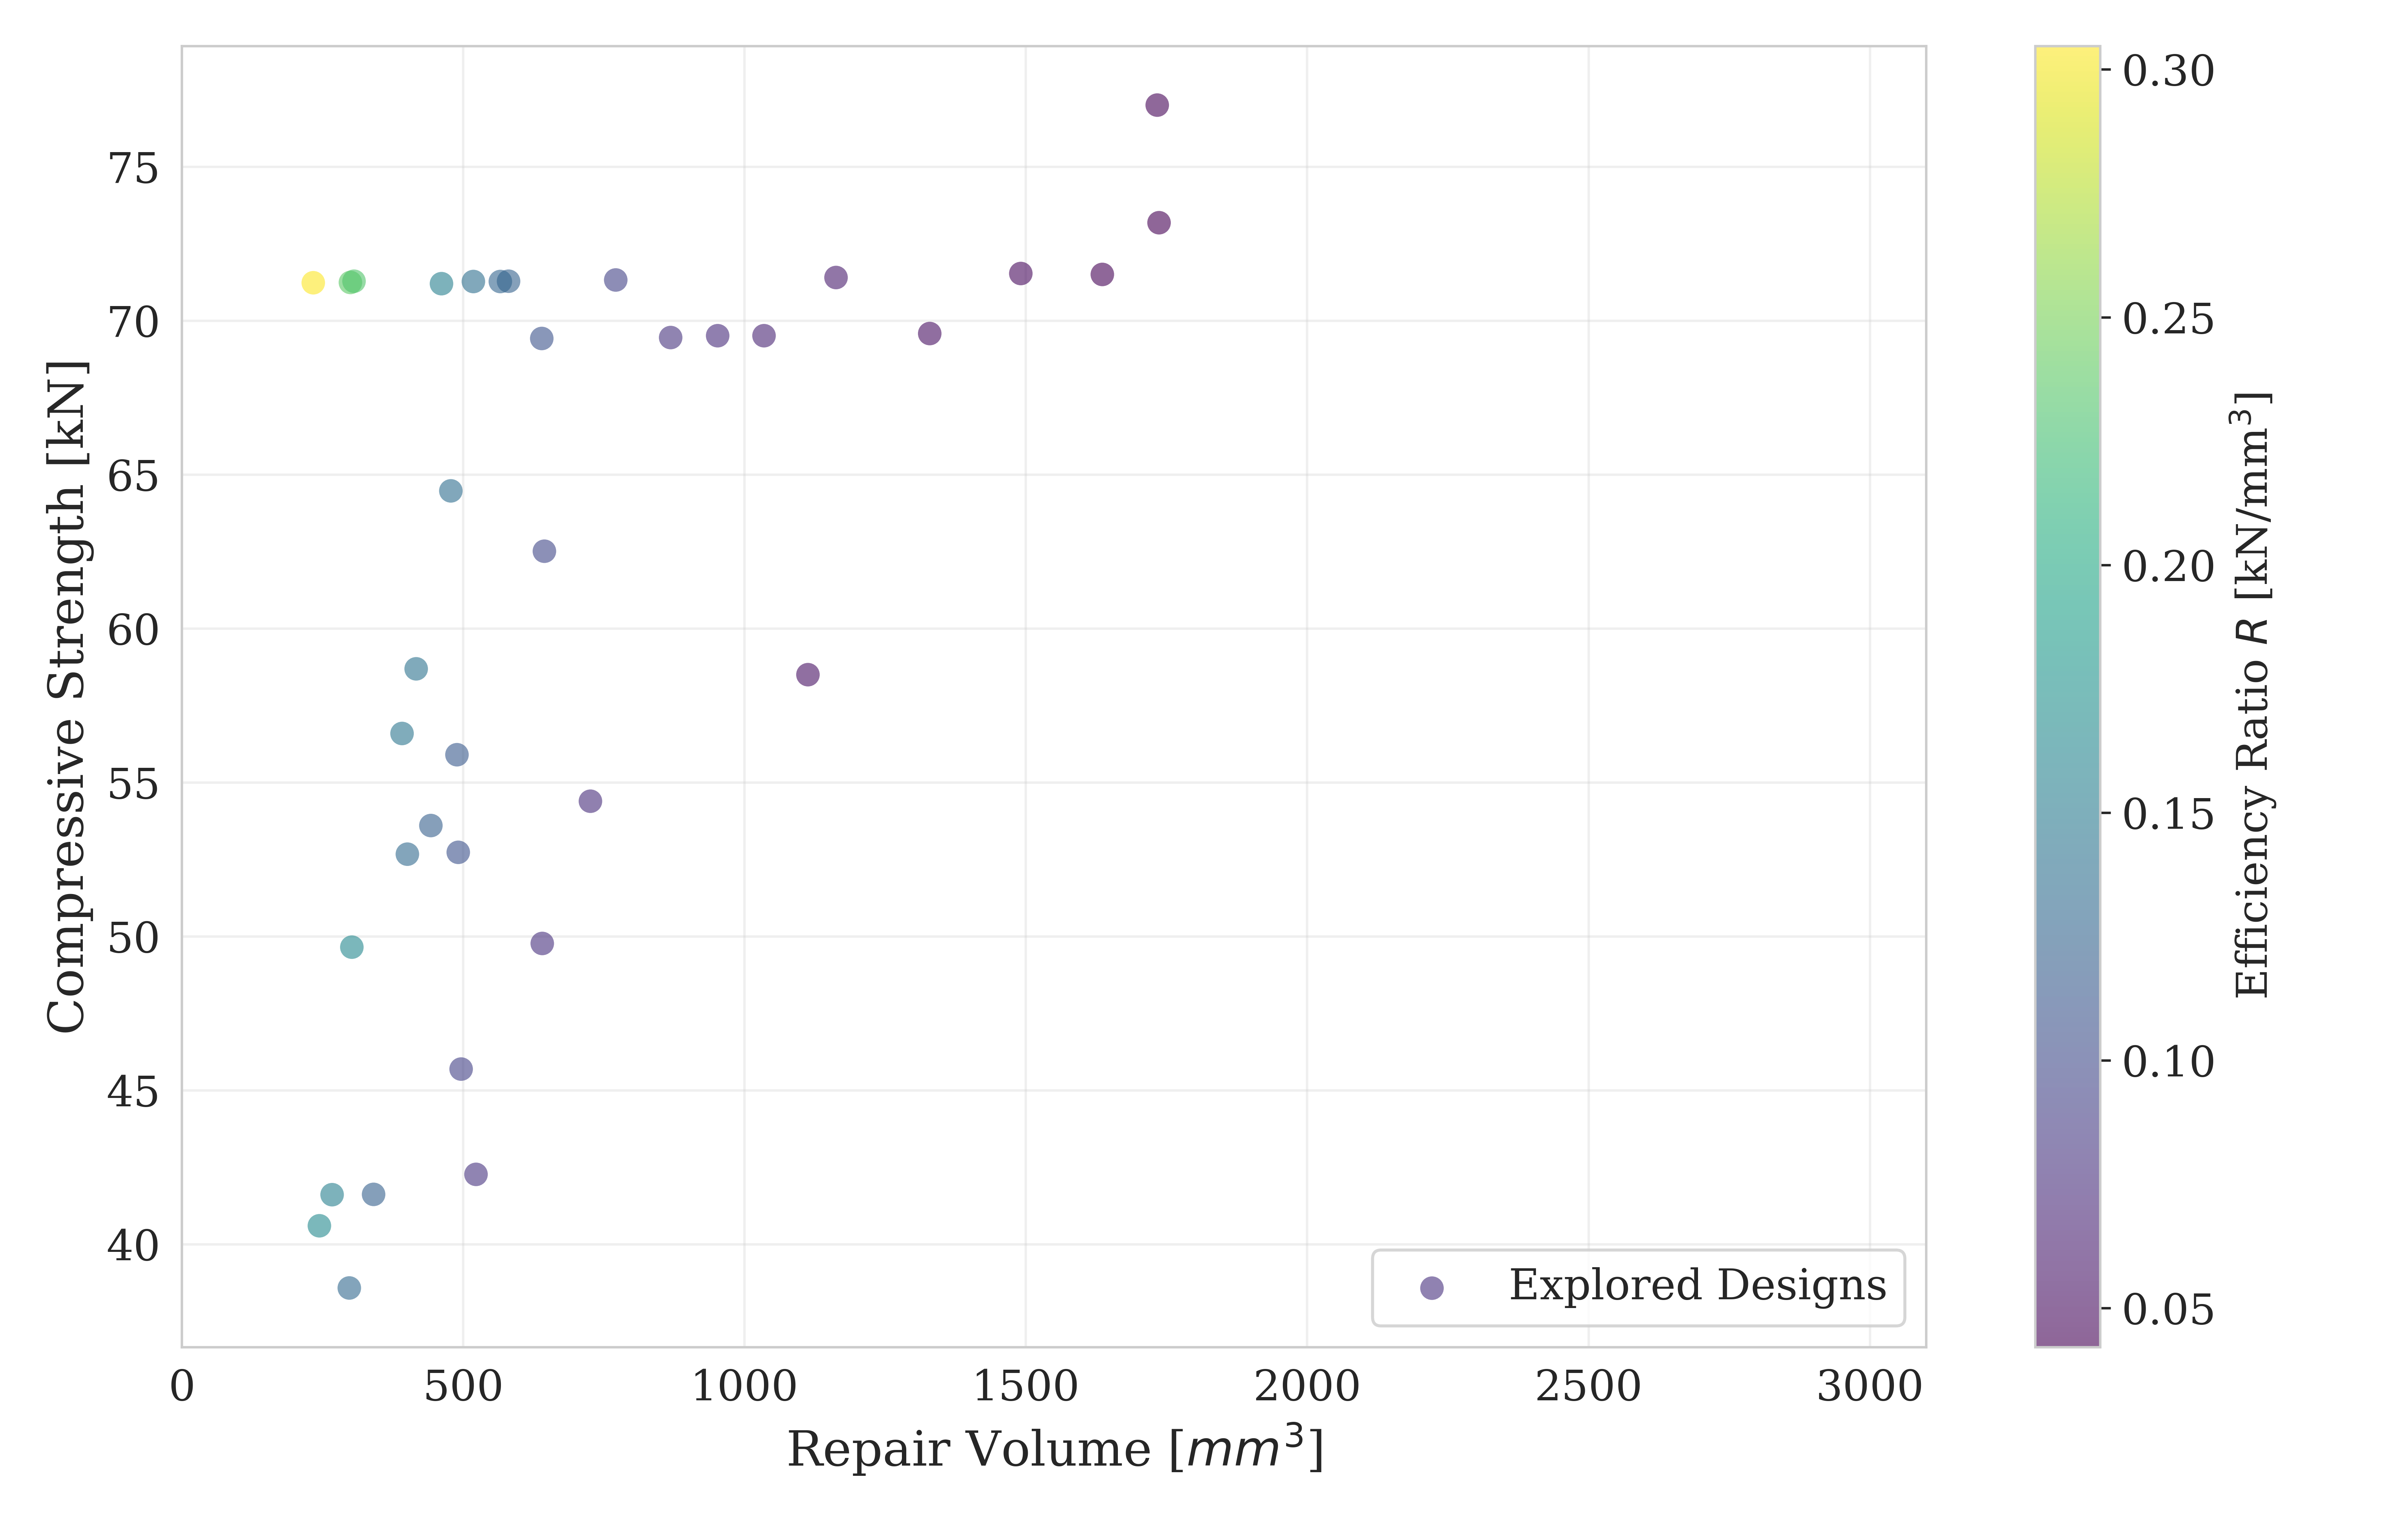
\includegraphics[width=\textwidth]{pre_activelearning_result_cat0_physics.png}
        \caption{Initial Random Sampling}
        \label{fig:cat0_pre}
    \end{subfigure}
    \hfill
    \begin{subfigure}[b]{0.49\textwidth}
        \centering
        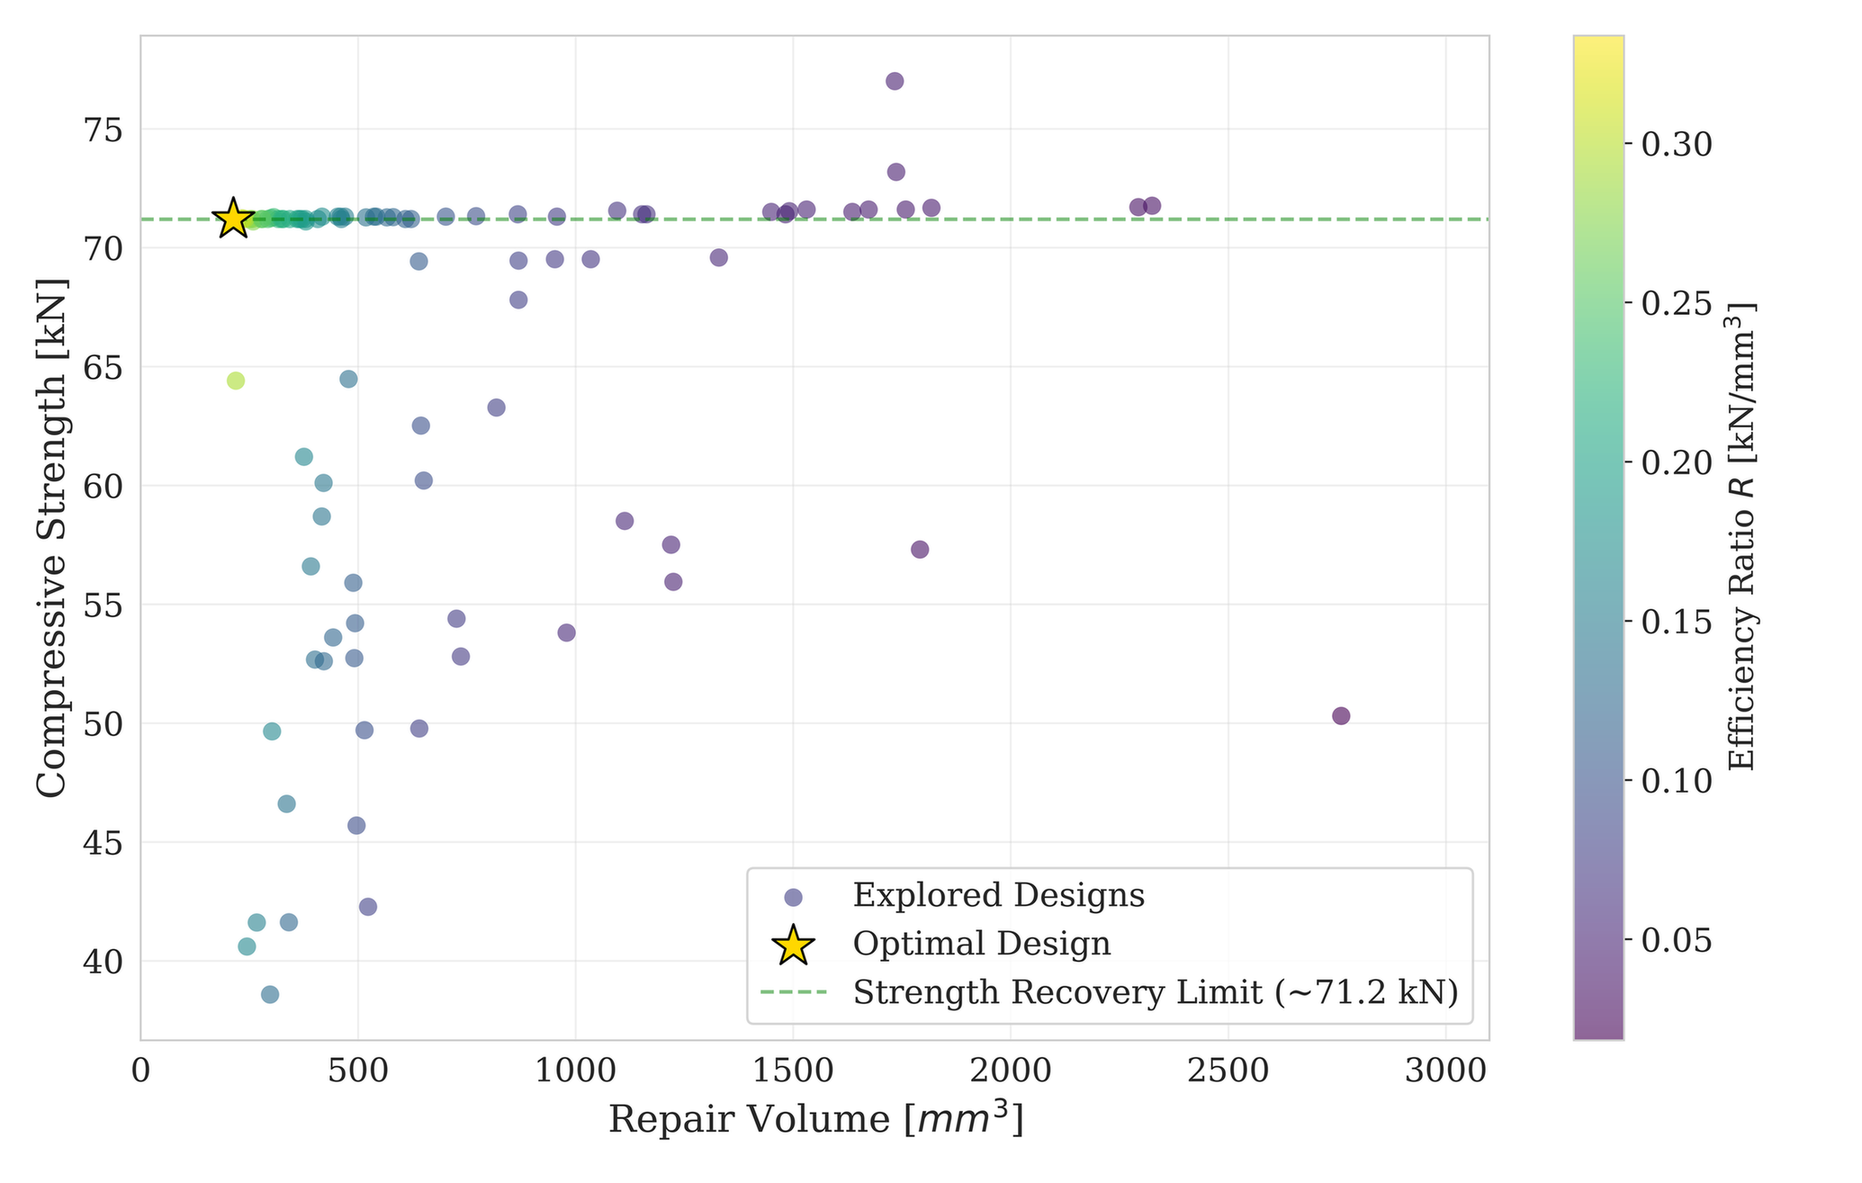
\includegraphics[width=\textwidth]{final_result_cat0_physics.png}
        \caption{Final Active Learning Result}
        \label{fig:cat0_final}
    \end{subfigure}
    \caption{Optimization results for Category 0. (a) The initial sampling shows high scatter. (b) The \new{active-learning loop} identifies a sharp "L-shaped" performance envelope bounded by the \new{strength-recovery limit}. The selection strategy targets the "knee" (Star), minimizing volume subject to reaching the maximum recoverable strength ($\approx 71.2$ kN).}
    \label{fig:cat0_results}
\end{figure}

The characteristic L-shape observed in Figure \ref{fig:cat0_final} arises because the objective space is physically bounded. While the pristine parent laminate possesses a strength of 75.0 kN, the stepped repair method inherently introduces stress concentrations at the corners of the excavated steps. Consequently, the strength recovery asymptotically saturates at a maximum recoverable limit of $\approx 71.2$ kN (roughly 95\% of the parent strength). This creates two distinct zones:
\begin{enumerate}
    \item \textbf{Vertical Leg} \new{(Pre-Saturation Zone)}: At lower volumes, strength increases rapidly with incremental material addition.
    \item \textbf{Horizontal Leg} (Saturation Zone): Once the \new{strength-recovery limit} ($\approx 95\%$) is reached, further increases in repair volume yield no structural benefit, resulting in a plateau of dominated designs.
\end{enumerate}

Given this saturation, the definition of the "Optimal Design" shifts from a continuous trade-off to a constrained minimization. We select the design located at the "knee" of the curve (marked with a Star). This candidate represents the global optimum: it is the design with the \textit{minimum} volume that successfully resides on the saturation plateau.

\textbf{Impact of Integer Constraints:}
It is observed that the transition at the "knee" of the Pareto front exhibits a slight discontinuity rather than a perfectly smooth curve. This is attributed to the discretization of the design space. To ensure manufacturing feasibility, the geometric parameters ($a_i, b_i$) were constrained to integers ($\mathbb{Z}$) in this framework, whereas previous parametric studies \cite{psarras2024design} allowed for decimal precision. The theoretical continuous Pareto front likely exists within the decimal intervals of these parameters . However, the \new{active-learning loop} successfully identified the best possible integer-constrained approximation, providing a robust solution ready for immediate manufacturing without rounding errors.

Finally, a critical physical insight was required to interpret the maximum load capacity. As observed in Figure \ref{fig:cat0_final}, several data points exhibit strength values exceeding 75 kN. These outliers are attributed to numerical artifacts in the explicit solver (Abaqus), likely resulting from kinetic energy oscillations during catastrophic failure. The framework, however, robustly identified the stable physical asymptote at 71.2 kN. Therefore, the "Optimal Design" was not selected by blindly taking the maximum numerical value, but by identifying the stable convergence point at the recovery limit with the lowest corresponding volume ($\approx 214.43$ mm$^3$).

\subsubsection{Category 1: \new{Mixed-Orientation Patches}}
The Category 1 optimization presented a more challenging landscape due to the presence of off-axis \new{patch plies}, which introduce coupled shear-extension failure modes. Figure \ref{fig:cat1_results} highlights the ability of the Deep Kernel to navigate this complexity.

\begin{figure}[htbp]
    \centering
    \begin{subfigure}[b]{0.49\textwidth}
        \centering
        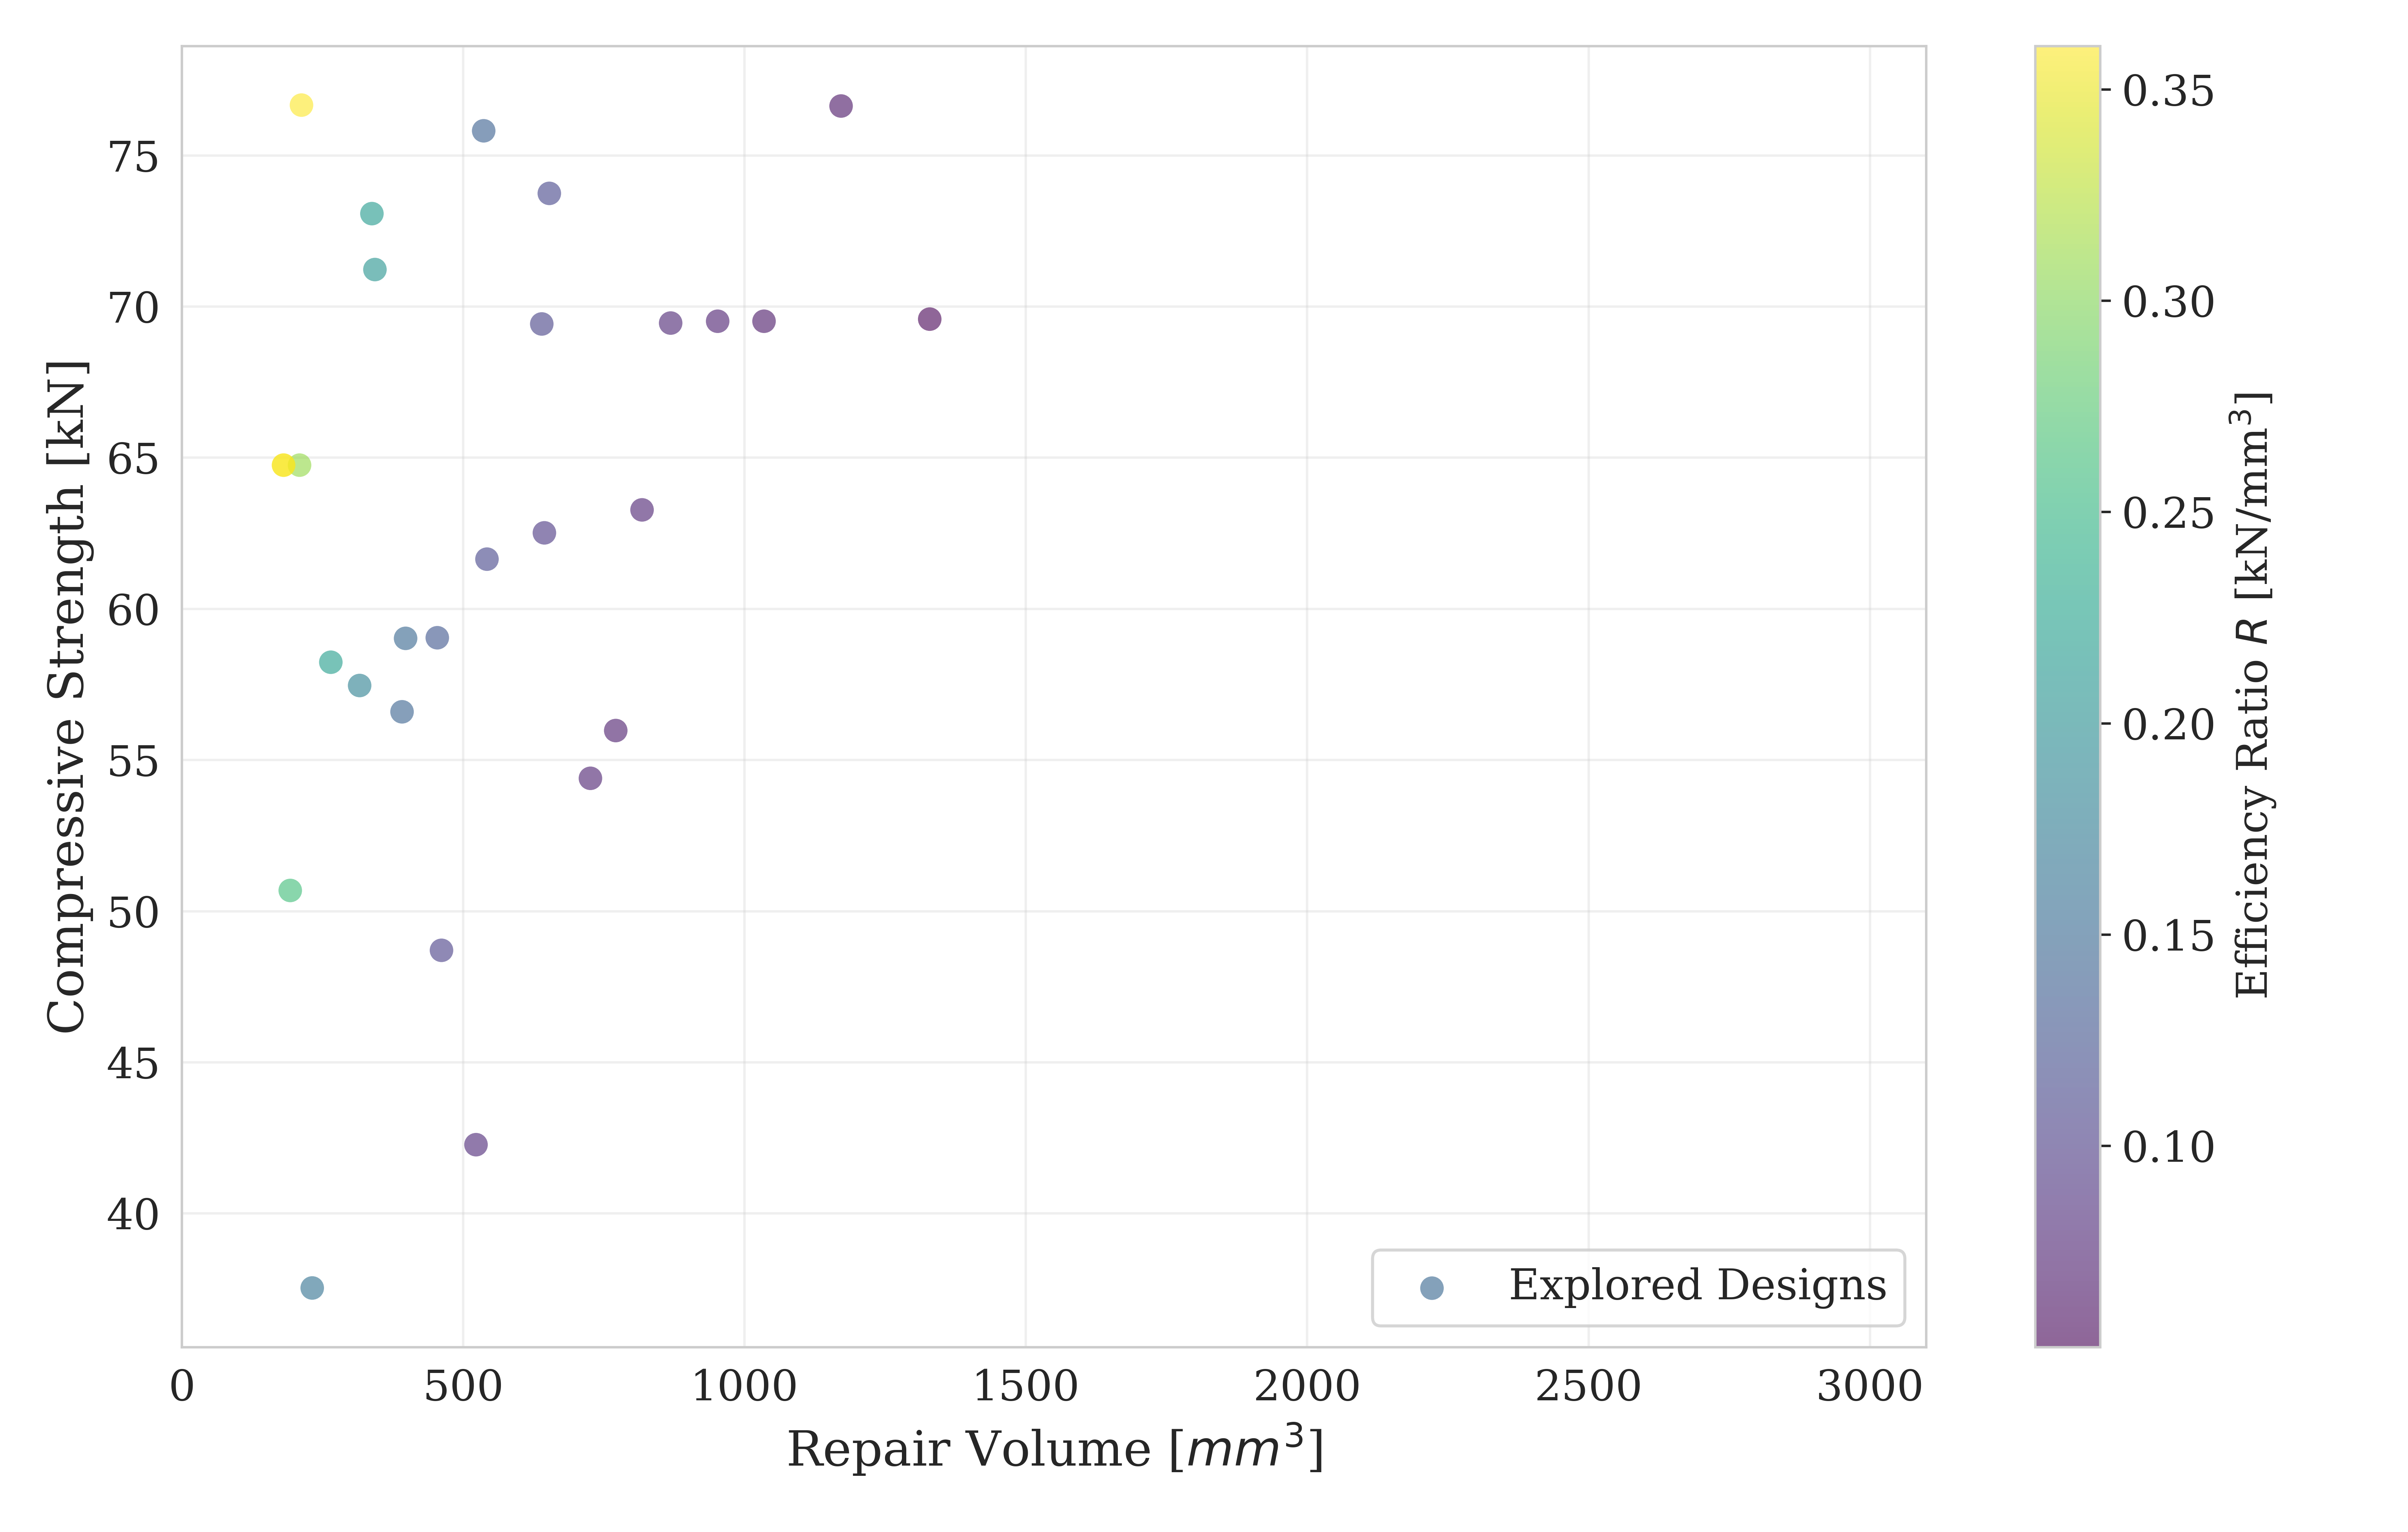
\includegraphics[width=\textwidth]{pre_activelearning_result_cat1_physics.png}
        \caption{Initial Random Sampling}
        \label{fig:cat1_pre}
    \end{subfigure}
    \hfill
    \begin{subfigure}[b]{0.49\textwidth}
        \centering
        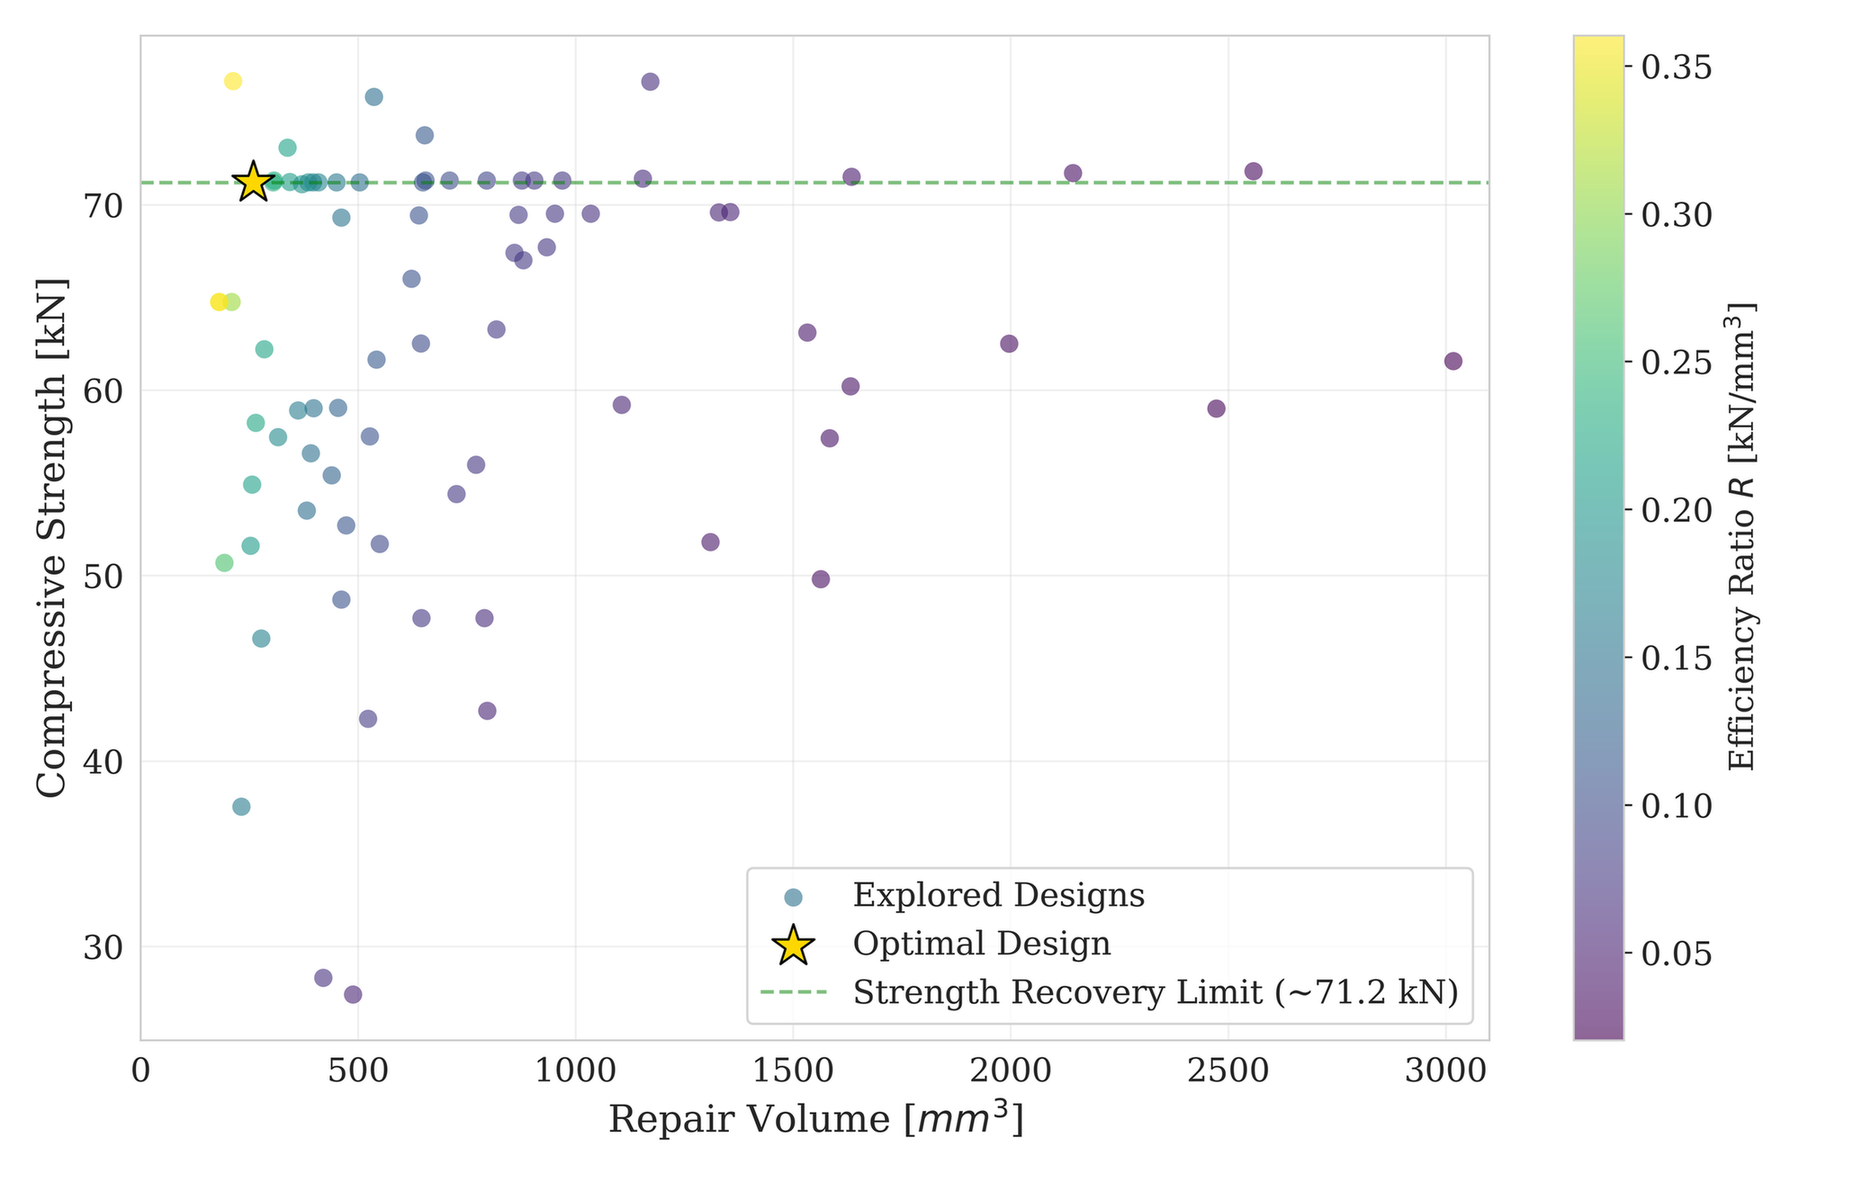
\includegraphics[width=\textwidth]{final_result_cat1_physics.png}
        \caption{Final Active Learning Result}
        \label{fig:cat1_final}
    \end{subfigure}
    \caption{Optimization results for Category 1. (a) Initial sampling results in \new{highly scattered strength-to-volume performance}. (b) The framework successfully pushes the Pareto frontier upward and to the left, identifying a high-efficiency design (Star) that maximizes strength recovery ($\approx 95\%$) despite the complex off-axis failure modes.}
    \label{fig:cat1_results}
\end{figure}

Despite the increased complexity, the Deep Kernel strategy successfully pushed the performance envelope upward and to the left. The plot reveals a clear distinction between the exploration phase, where the algorithm discarded large, inefficient geometries, and the exploitation phase, where it focused on tuning the aspect ratios of smaller patches.

Similar to Category 0, the selection of the optimal design (Gold Star) prioritized physical validity. The selected design restores 71.0 kN (approximately 95\% recovery relative to the 75.0 kN parent strength) while maintaining a compact volume. This result confirms that \new{near-maximal strength recovery} is achievable even with mixed-modality repairs if the shear-extension coupling is mitigated through precise geometric tuning.


% --- Discussion Text ---
\subsection{Analysis of Search Efficiency and Model Convergence}
Tables \ref{tab:cat0_candidates} and \ref{tab:cat1_candidates} present the top performing candidates for both categories. \new{In what follows, ``Run~$N$'' refers to the $N$-th active-learning iteration (counting the first FEM evaluation proposed by the surrogate as Run~1), while ``Init.\,Spec.~$K$'' refers to the $K$-th design from the warm-start dataset (the 38 Category~0 and 28 Category~1 seed designs from the prior parametric study).} While both categories achieve a similar peak strength ($\approx 71.2$ kN), Category 0 clearly exhibits superior \new{material-use efficiency} (higher strength recovered per unit removed volume).

% --- Table for Category 0 ---
\begin{table}[htbp]
    \centering
    \caption{Top 4 Candidates: Category 0 \new{(Aligned-Orientation Patches)}}
    \label{tab:cat0_candidates}
    \begin{tabular}{l c c c}
        \toprule
        \textbf{Candidate ID} & \textbf{Strength (kN)} & \textbf{Volume ($mm^3$)} & \textbf{\new{Strength-to-Volume Ratio $R$ [kN/mm$^3$]}} \\
        \midrule
        Run 8 & 71.20 & 214.43 & \textbf{0.332} \\
        Init.Spec.16 & 71.23 & 234.99 & 0.303 \\
        Run 47 & 71.20 & 236.17 & 0.301 \\
        Run 40 & 71.20 & 241.45 & 0.295 \\
        \bottomrule
    \end{tabular}
\end{table}

% --- Table for Category 1 ---
\begin{table}[htbp]
    \centering
    \caption{Top 4 Candidates: Category 1 \new{(Mixed-Orientation Patches)}}
    \label{tab:cat1_candidates}
    \begin{tabular}{l c c c}
        \toprule
        \textbf{Candidate ID} & \textbf{Strength (kN)} & \textbf{Volume ($mm^3$)} & \textbf{\new{Strength-to-Volume Ratio $R$ [kN/mm$^3$]}} \\
        \midrule
        Run 42 & 71.20 & 260.84 & \textbf{0.273} \\
        Run 36 & 71.20 & 306.66 & 0.232 \\
        Run 23 & 71.30 & 308.43 & 0.231 \\
        Init.Spec. 9 & 71.22 & 345.17 & 0.206 \\
        \bottomrule
    \end{tabular}
\end{table}


Beyond the performance metrics, the optimization timeline reveals a significant difference in how the algorithm navigated the two design spaces. For Category 0, the optimal candidate was identified just \textbf{8 runs} after the \new{warm-start dataset} was established. This suggests that the relationship between the standard geometric parameters and performance was relatively linear, allowing the model to converge quickly.

In contrast, the best candidate for Category 1 was not found until \textbf{42 runs} into the process. This delay can be attributed to the gradual increase in model complexity required to understand Category 1. In the early stages, the surrogate model likely lacked the predictive performance to capture the non-linear complexities and geometric "jumps" inherent in Category 1. Consequently, the algorithm required a significantly larger exploration phase to accumulate enough data to accurately map the design space and locate the optimal solution.

\subsubsection{Benchmarking Computational Efficiency}
While a direct head-to-head comparison with a global optimizer was operationally infeasible due to the extreme computational cost of the high-fidelity FEM (approx. 3 hours per run), the \new{computational speed-up} can be quantified against established baselines. 

For a 12-dimensional design space, a naive full-factorial Grid Search (even at a coarse resolution of 3 levels) would require $3^{12} \approx 5.3 \times 10^5$ evaluations, rendering it computationally intractable. Standard derivative-free algorithms like Genetic Algorithms (GA) typically require a population size of approx. 50 evolved over 50 generations, implying a budget of $\mathbf{2,500}$ evaluations to ensure robust convergence \cite{queipo2005surrogate}. Even efficient static sampling methods such as Latin Hypercube Sampling (LHS) generally require hundreds of samples ($>500$) to sufficiently dense-pack the design space and resolve narrow high-performance regions without the guidance of an acquisition function.

In stark contrast, the \new{DKAL framework} converged to the maximum recoverable strength ($\approx 95\%$) in just 59 total evaluations for Category 0 and 92 evaluations for Category 1. Comparing this sample efficiency to the GA baseline suggests a computational reduction of approximately 96\%, and an improvement of roughly 80--90\% over static sampling strategies. This result aligns with findings in similar composite optimization studies, where Bayesian Optimization consistently outperforms evolutionary strategies by an order of magnitude in data-sparse regimes \cite{ghosh2023digital}.


% --- FIGURE 1: CATEGORY 0 EVOLUTION ---
\begin{figure}[htbp]
    \centering
    % Top Subfigure: Parameter Heatmap
    \begin{subfigure}[b]{\textwidth}
        \centering
        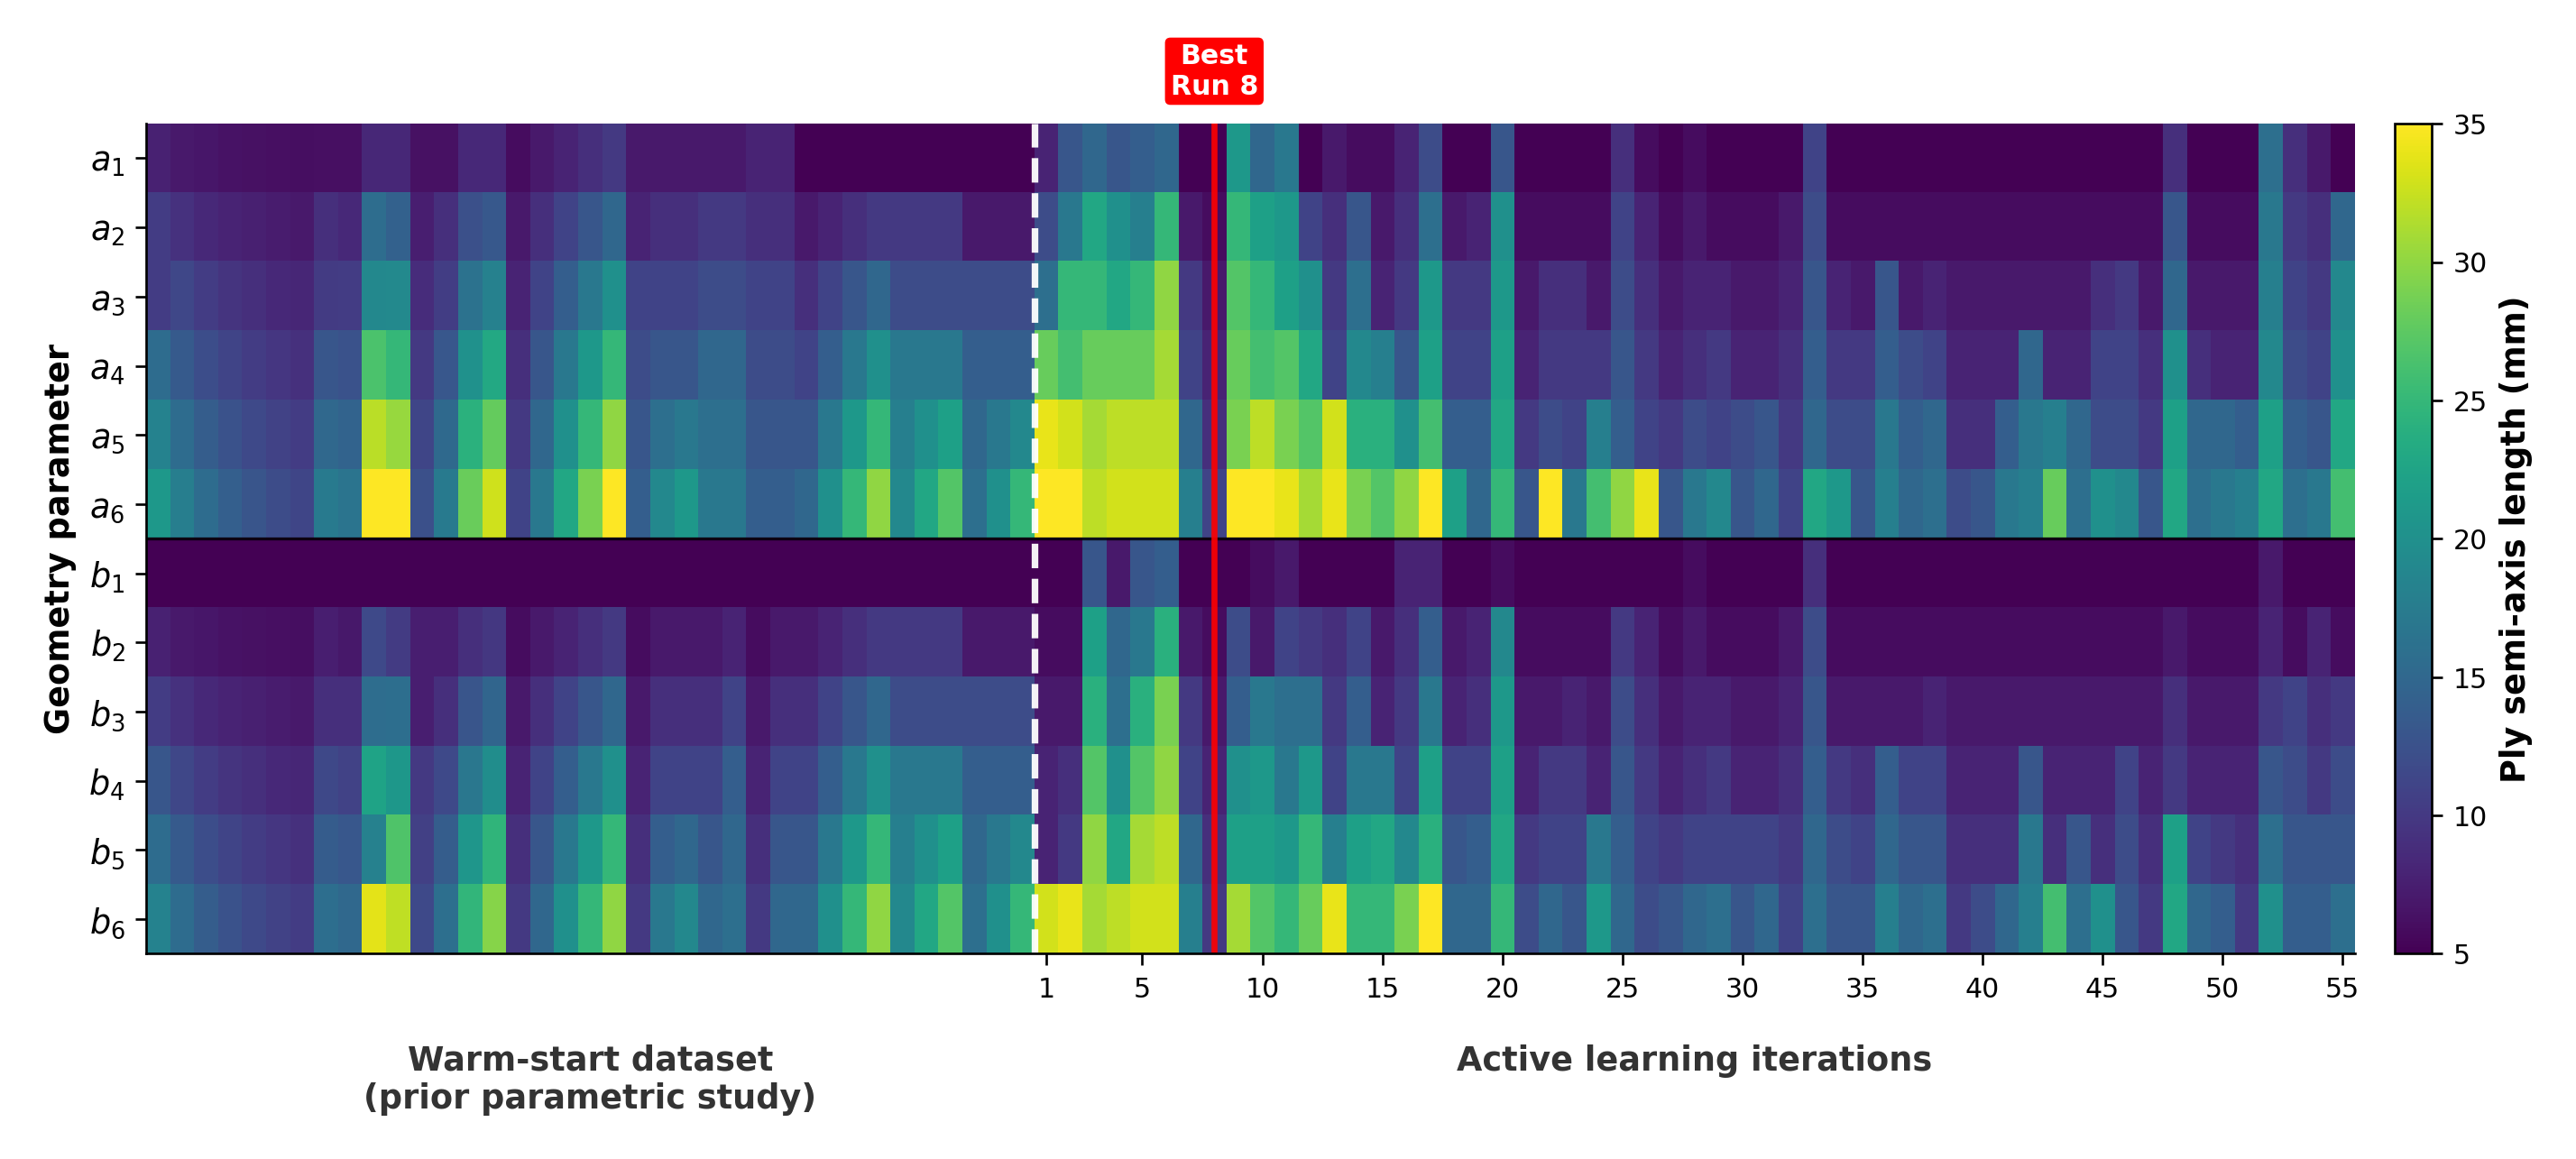
\includegraphics[width=\linewidth]{parameter_evolution_cat0.png}
        \caption{Evolution of Geometry Parameters (Heatmap)}
        \label{fig:cat0_heatmap}
    \end{subfigure}
    
    \par\vspace{0.5cm} % Adds vertical breathing room between the plots
    
    % Bottom Subfigure: Performance Triplet
    \begin{subfigure}[b]{\textwidth}
        \centering
        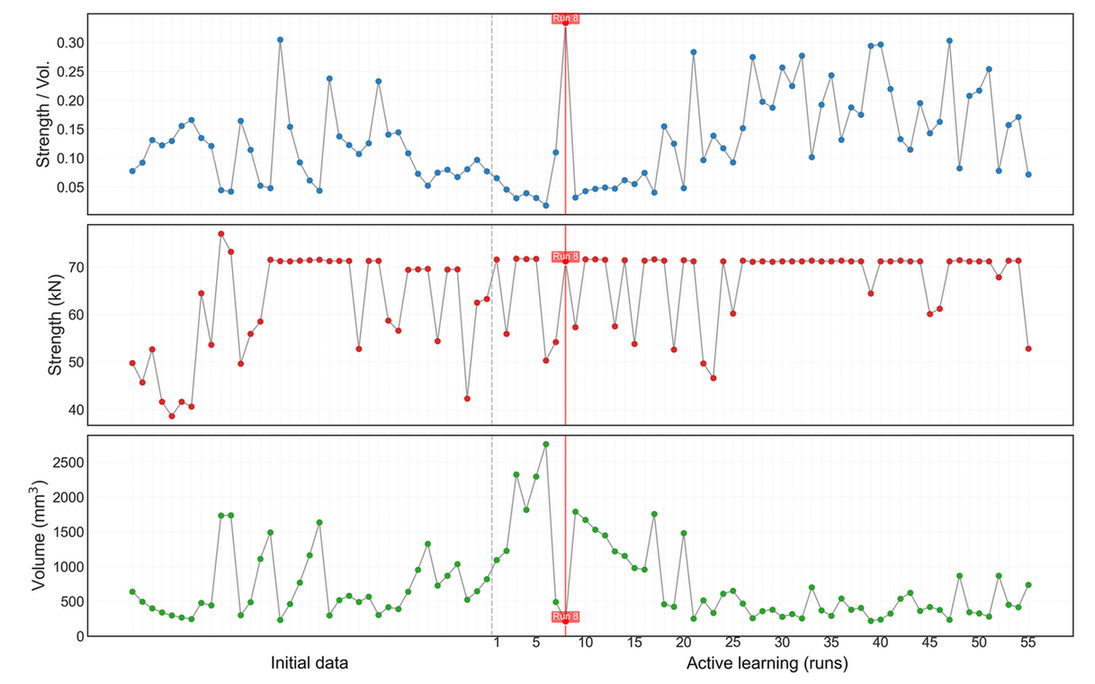
\includegraphics[width=\linewidth]{performance_triplet_cat0.png}
        \caption{Evolution of Performance Metrics (Strength/Volume Ratio, Strength, Volume)}
        \label{fig:cat0_triplet}
    \end{subfigure}
    
    \caption{\textbf{Category 0 Convergence Profile.} \new{The parameter heatmap (a) shows the 12 patch-ply semi-axes (rows) over time (columns): the warm-start dataset (left of the white dashed line, 38 designs from the prior parametric study) feeds the active-learning iterations (right of the white dashed line). Each cell colour is the value of one parameter in mm; the colorbar gives the scale. The red vertical line marks the best candidate, found at Run 8.} The performance metrics (b) confirm this early peak in the \new{strength-to-volume ratio}.}
    \label{fig:cat0_evolution}
\end{figure}

% --- FIGURE 2: CATEGORY 1 EVOLUTION ---
\begin{figure}[htbp]
    \centering
    % Top Subfigure: Parameter Heatmap
    \begin{subfigure}[b]{\textwidth}
        \centering
        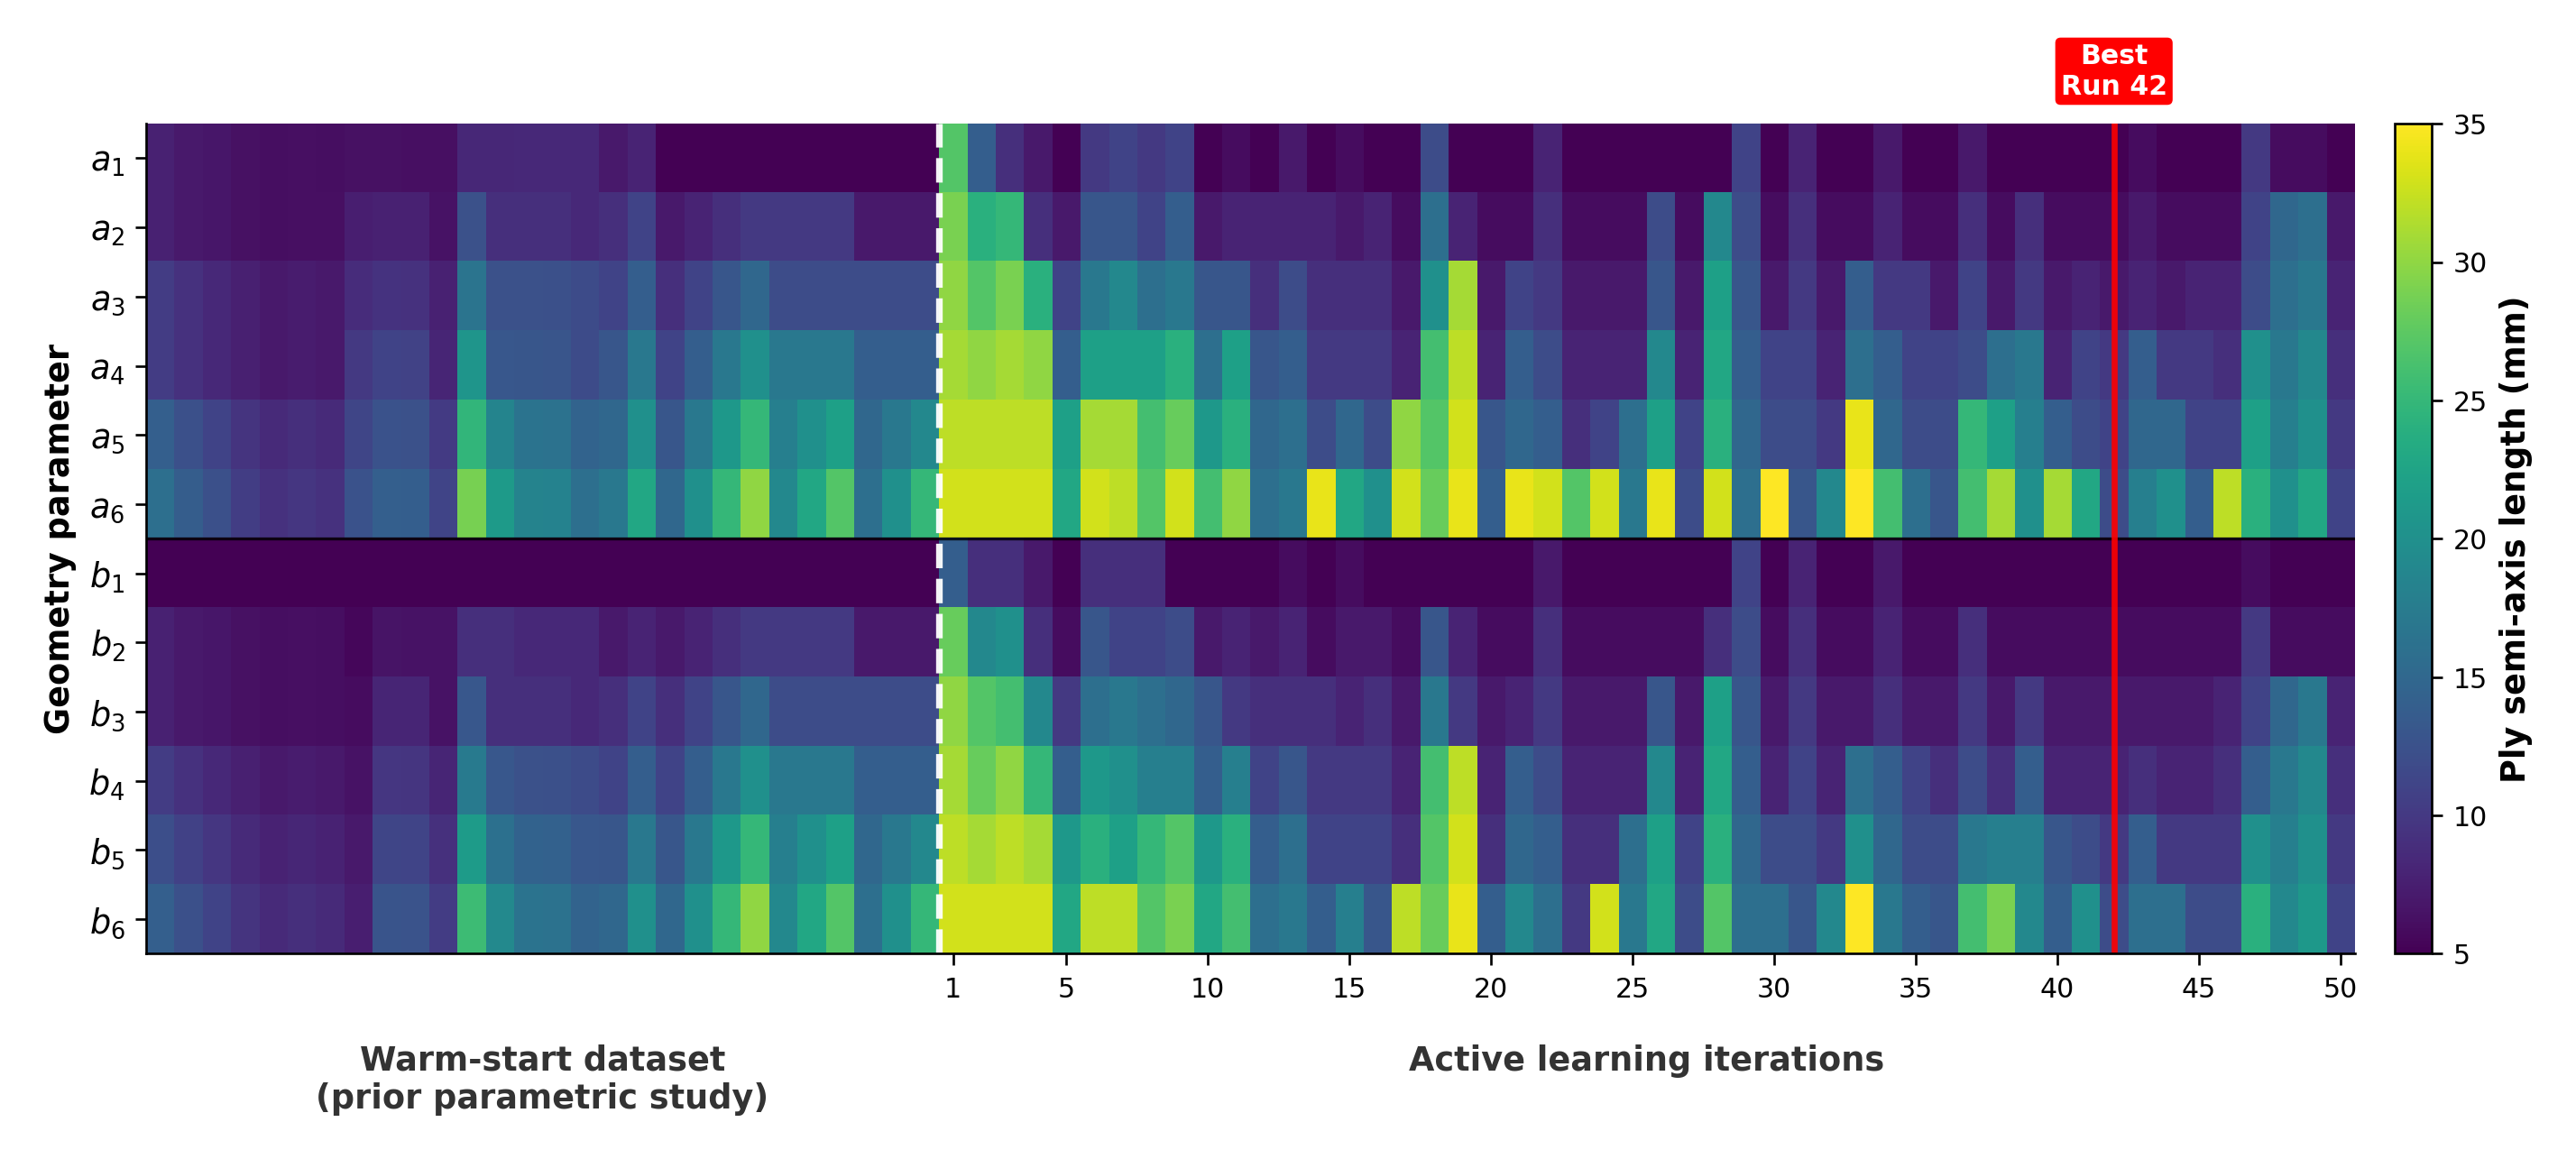
\includegraphics[width=\linewidth]{parameter_evolution_cat1.png}
        \caption{Evolution of Geometry Parameters (Heatmap)}
        \label{fig:cat1_heatmap}
    \end{subfigure}
    
    \par\vspace{0.5cm} % Adds vertical breathing room between the plots
    
    % Bottom Subfigure: Performance Triplet
    \begin{subfigure}[b]{\textwidth}
        \centering
        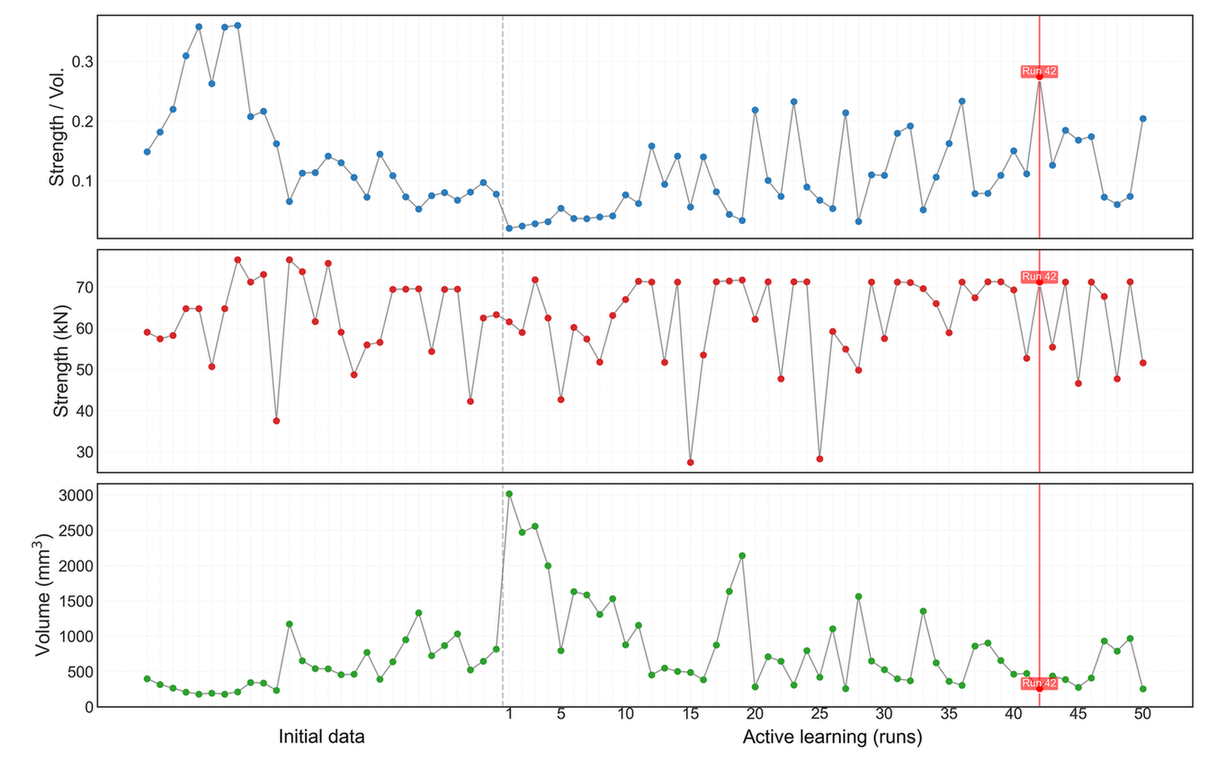
\includegraphics[width=\linewidth]{performance_triplet_cat1.png}
        \caption{Evolution of Performance Metrics (Strength/Volume Ratio, Strength, Volume)}
        \label{fig:cat1_triplet}
    \end{subfigure}
    
    \caption{\textbf{Category 1 Convergence Profile.} \new{Same convention as Fig.~\ref{fig:cat0_evolution}: the parameter heatmap (a) shows the 12 patch-ply semi-axes over the 28-design warm-start dataset (prior parametric study, left of the white dashed line) and the 50 subsequent active-learning iterations (right). The red vertical line marks the best candidate, found here at Run 42 --- much later than Cat 0, reflecting the prolonged volatility of the parameter map under the off-axis (mixed-orientation) failure mechanics.} The optimal candidate is not identified until Run 42, reflecting the difficulty in mapping the complex, high-volume design space shown in (b).}
    \label{fig:cat1_evolution}
\end{figure}

\subsection{Visualizing the Convergence Gap}

The disparity in search efficiency is visually confirmed by the evolutionary plots in Figure \ref{fig:cat0_evolution} and Figure \ref{fig:cat1_evolution}.

\subsubsection{Category 0 (Figure \ref{fig:cat0_evolution})}
\new{Figure~\ref{fig:cat0_evolution}(a) shows that in the warm-start region (left of the white dashed line, 38 designs from the prior parametric study \cite{psarras2024design}) the design space is dominated by bright bands in the outer patch-ply parameters $a_5, a_6, b_5, b_6$ -- i.e.\ the prior parametric study explored large patches. Once the active-learning loop takes over (right of the white dashed line), the proposed designs settle within $\sim$20 iterations into a stable, low-variance configuration concentrated in the small-dimension regime; the optimal candidate is identified at Run 8 (vertical red line). The performance triplet in Fig.~\ref{fig:cat0_evolution}(b) confirms this: the strength-to-volume ratio peaks sharply at Run 8 and the design lock-on is visible as nearly-flat parameter traces beyond Run~20.}

\subsubsection{Category 1 (Figure \ref{fig:cat1_evolution})}
\new{In contrast, Figure~\ref{fig:cat1_evolution}(a) shows that for the mixed-orientation Category~1 case the parameter map remains volatile well into the active-learning phase: bright/dark transitions in $a_3$--$a_6$ and $b_3$--$b_6$ persist through the first $\sim$40 iterations, indicating that the surrogate had not yet localised the optimal geometry.} The performance plots (Fig. \ref{fig:cat1_evolution}b) reveal that during this search, the \new{active-learning loop} encountered a highly non-linear response surface, characterized by sharp drops in residual strength to approximately \textbf{27--30 kN}.

Finite Element analysis of these low-performing candidates reveals that the failure is driven by premature adhesive debonding rather than ply failure. As visualized in Figure \ref{fig:debonding_comparison}a, the Contact Status output for a failed candidate shows extensive "Open" regions (Blue), indicating that the patch separated from the parent laminate before significant load transfer could occur. This suggests that certain geometric combinations in the off-axis design space trigger a transition from stable shear transfer to unstable peeling. 

In contrast, the optimal candidate identified later in the process (Figure \ref{fig:debonding_comparison}b) maintains a fully closed "Sticking" status (Red) up to the failure load. This confirms that the \new{active-learning loop} successfully learned to navigate this bifurcation, identifying the narrow geometric corridor that mitigates early decohesion and enables full strength recovery ($>71$ kN).


\begin{figure}[htbp]
    \centering
    \begin{subfigure}[b]{0.49\textwidth}
        \centering
        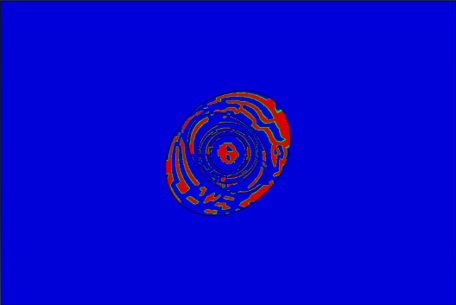
\includegraphics[width=\textwidth]{Failed_Debonding_27kN.png}
        \caption{Premature Failure (27.4 kN) - Run 15}
        \label{fig:fail_27kN}
    \end{subfigure}
    \hfill
    \begin{subfigure}[b]{0.49\textwidth}
        \centering
        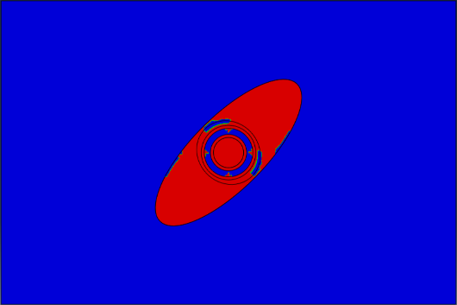
\includegraphics[width=\textwidth]{Optimal_Bond_71kN.png}
        \caption{Optimal Strength (71.2 kN) - Run 46}
        \label{fig:opt_71kN}
    \end{subfigure}
    \caption{Finite Element visualization of the adhesive contact status (Red: Sticking, Green: Slipping, Blue: Open/Debonded). (a) An inefficient AI-generated candidate suffers from excessive peel stresses, leading to debonding at only 27.4 kN. (b) The optimal design identified by the Deep Kernel maintains full adhesive contact (Red), achieving the maximum recoverable strength.}
    \label{fig:debonding_comparison}
\end{figure}





% --- FIGURE 3: CATEGORY 0 TOP CANDIDATES (GEOMETRY) ---
\begin{figure}[htbp]
    \centering
    % Row 1
    \begin{subfigure}[b]{0.48\textwidth}
        \centering
        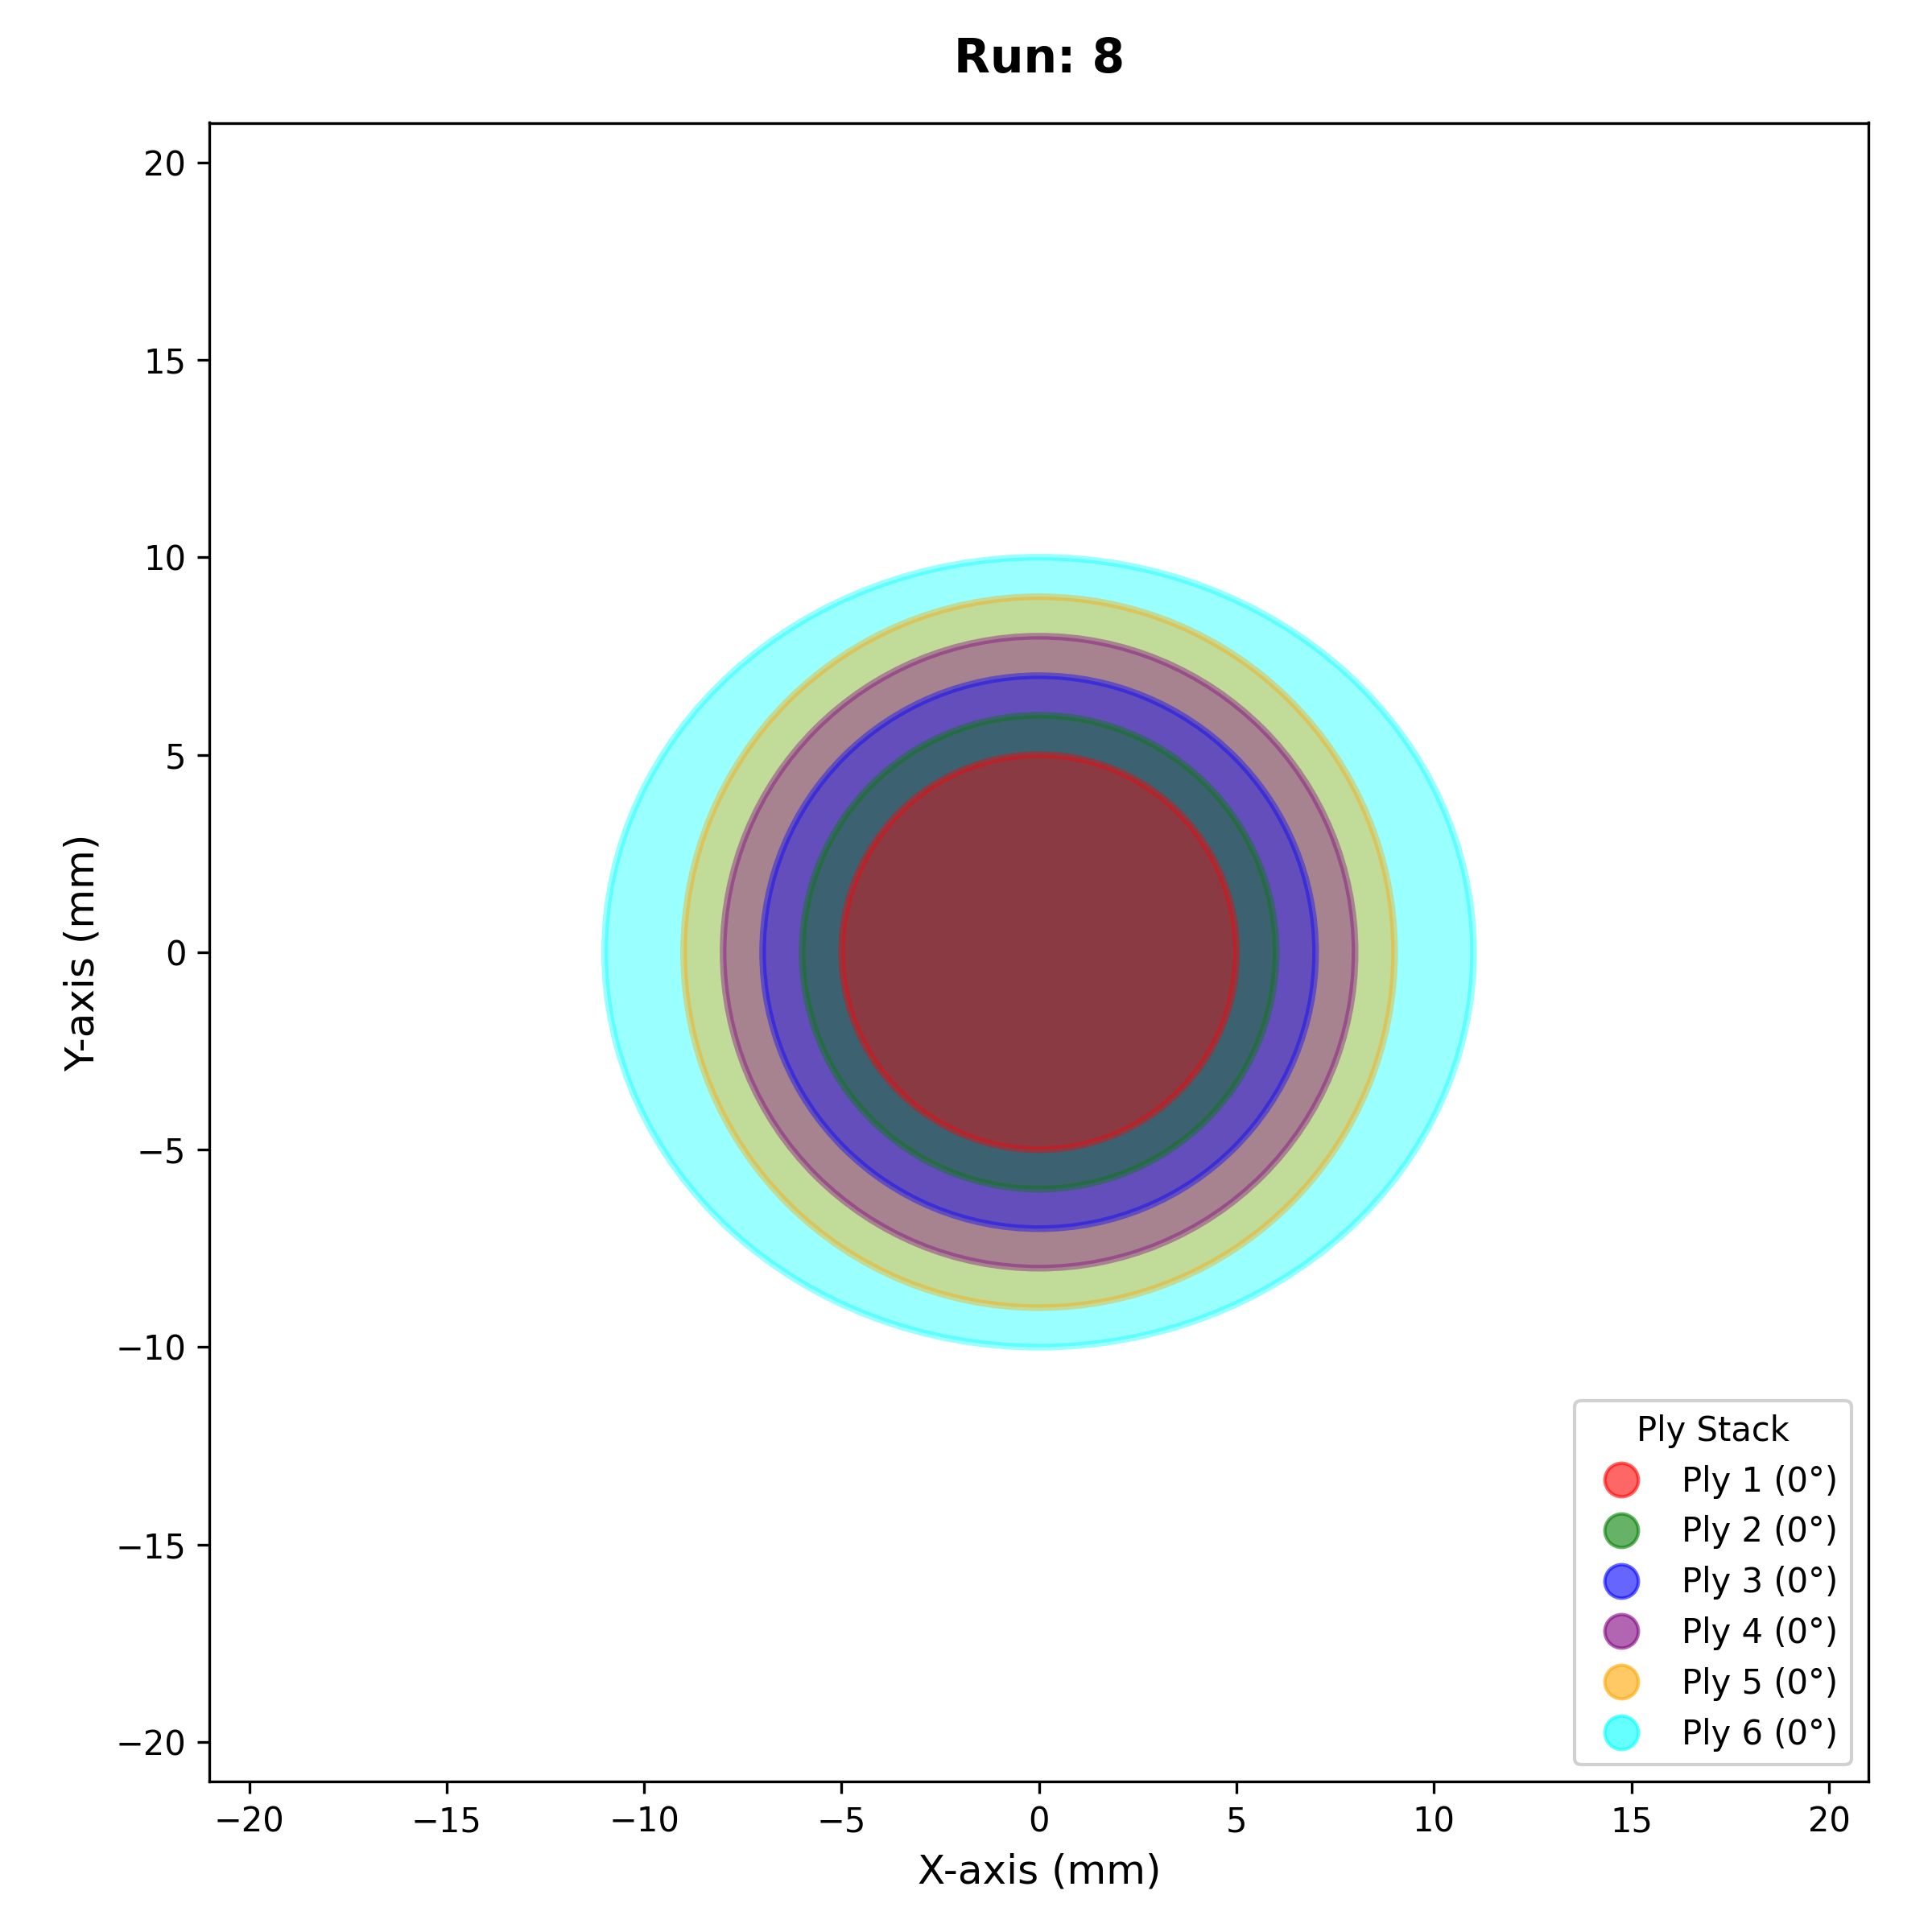
\includegraphics[width=\linewidth]{top_view_Cat0.0_Row0.png}
        \caption{Best Candidate: Run 8}
        \label{fig:cat0_best}
    \end{subfigure}
    \hfill
    \begin{subfigure}[b]{0.48\textwidth}
        \centering
        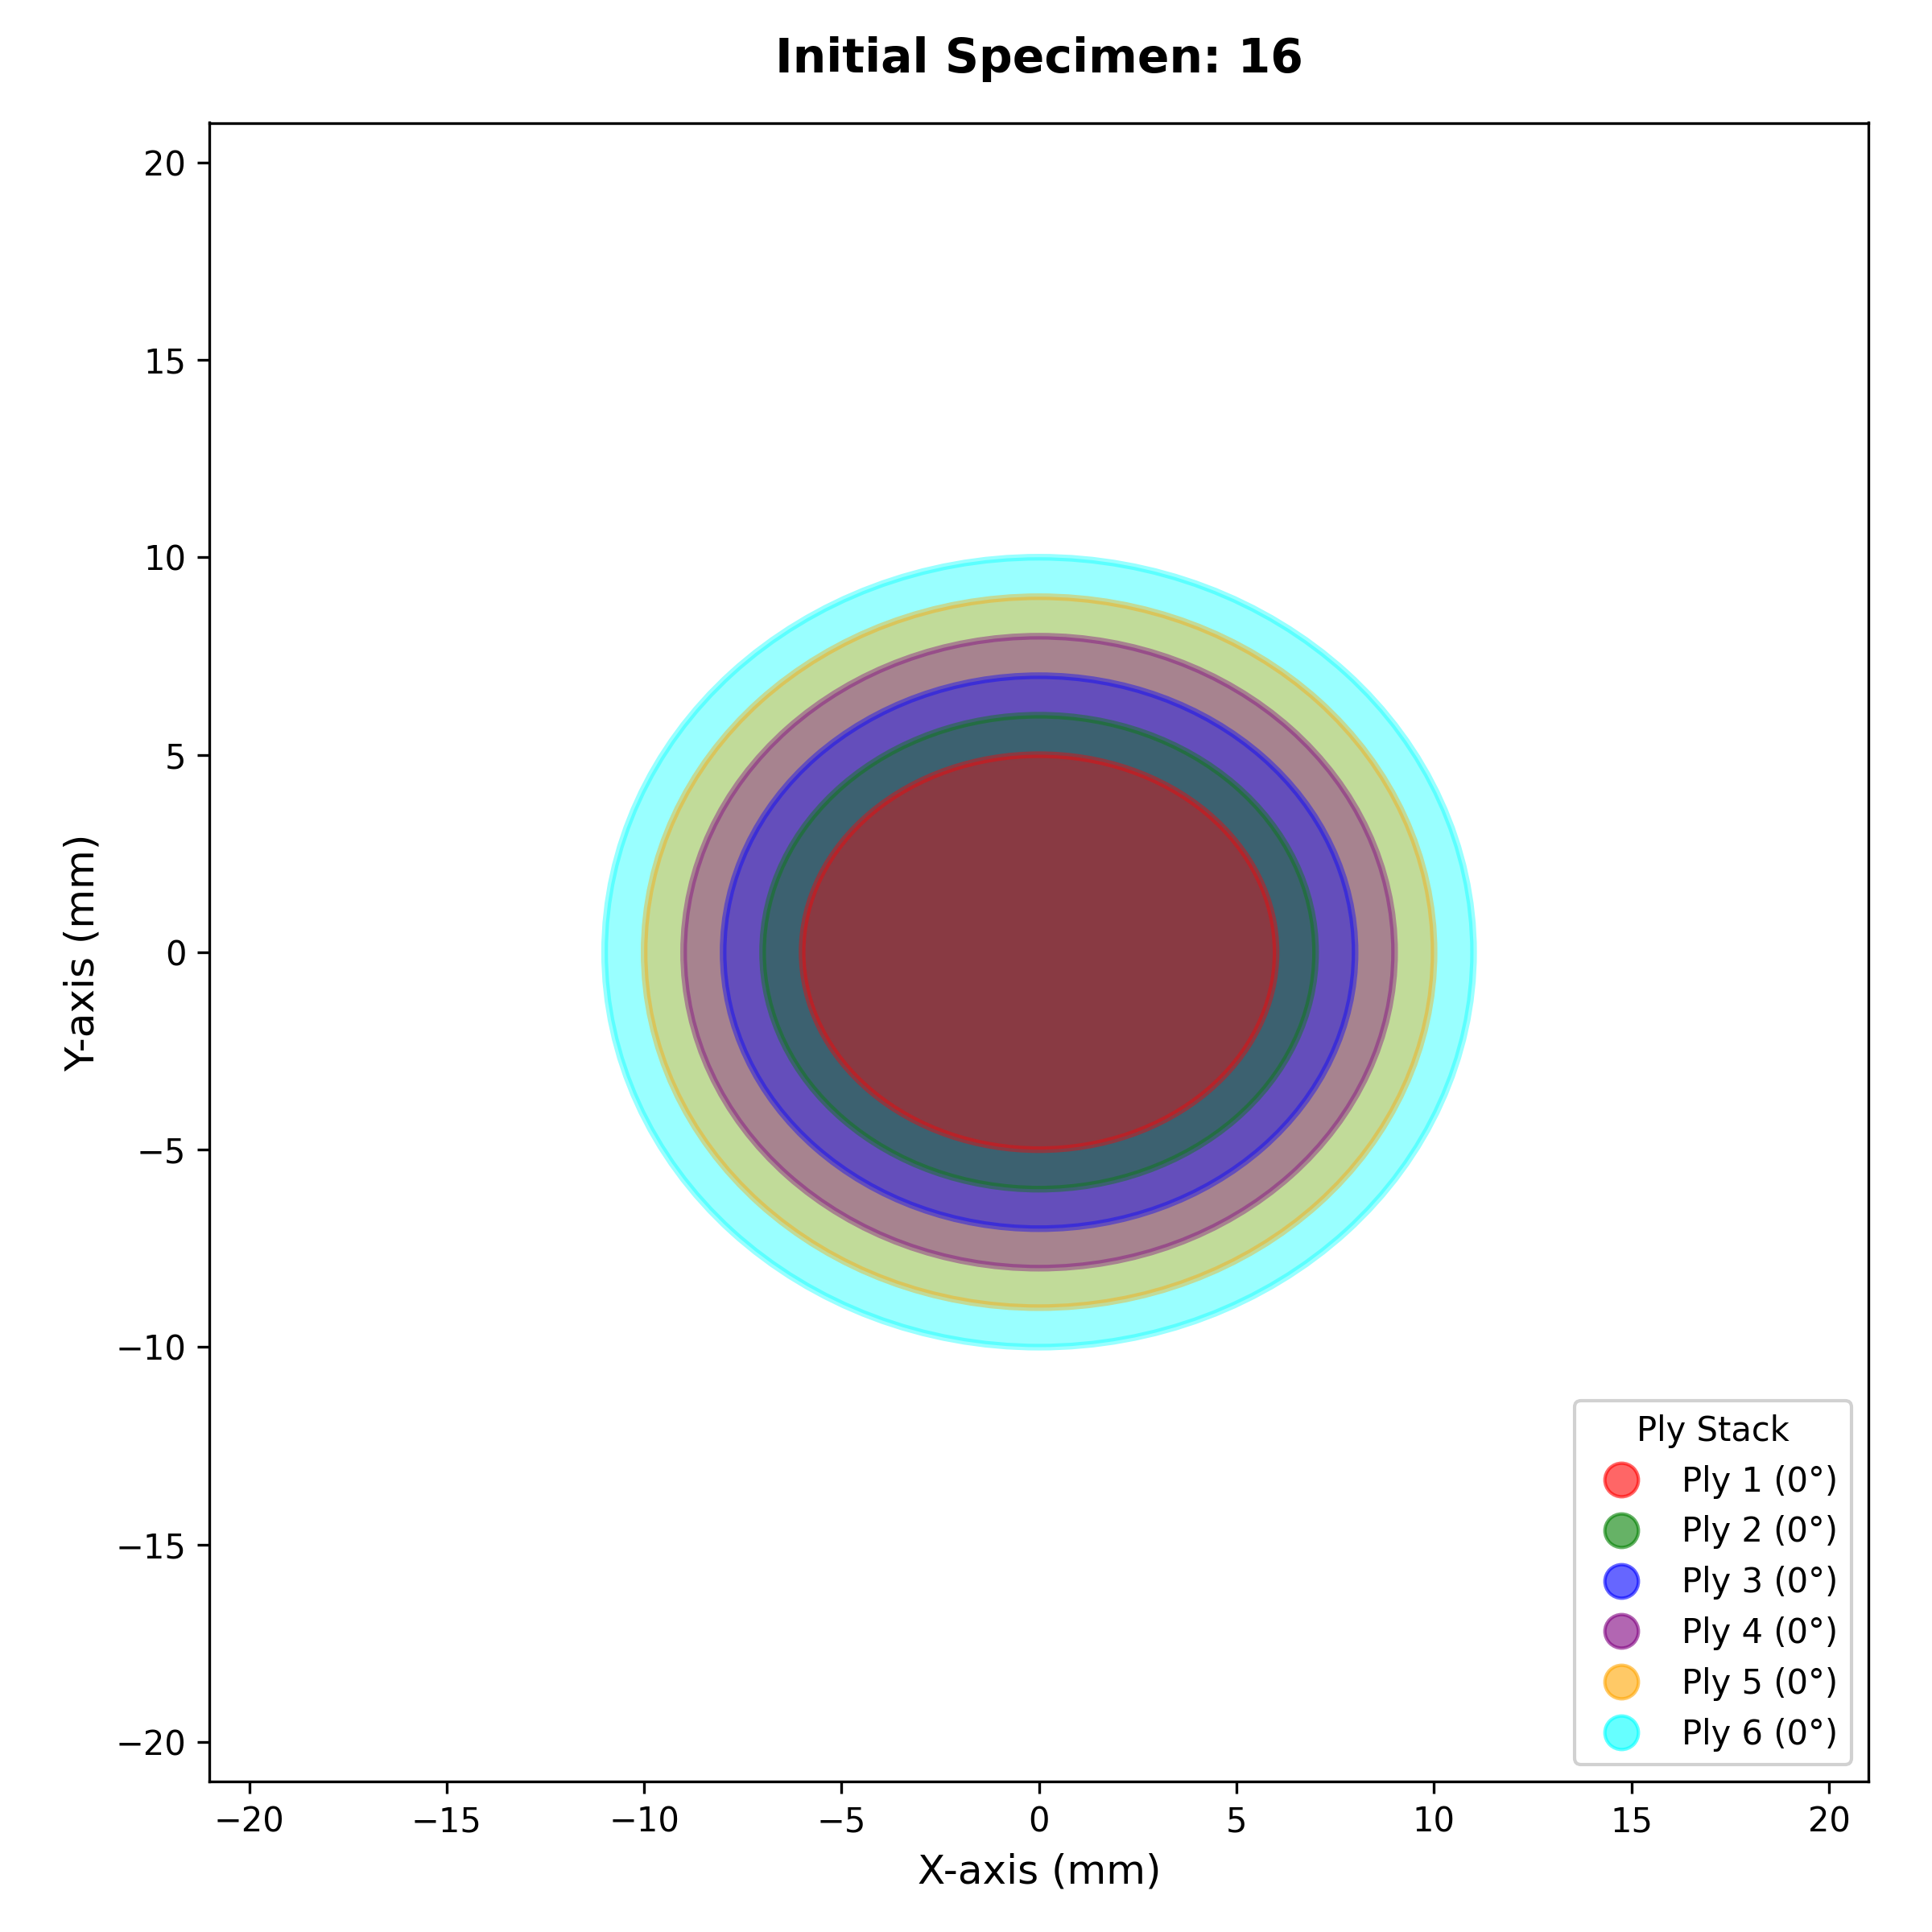
\includegraphics[width=\linewidth]{top_view_Cat0.0_Row1.png}
        \caption{Initial Specimen 16}
        \label{fig:cat0_initial}
    \end{subfigure}
    
    \par\vspace{0.5cm} % Vertical spacing
    
    % Row 2
    \begin{subfigure}[b]{0.48\textwidth}
        \centering
        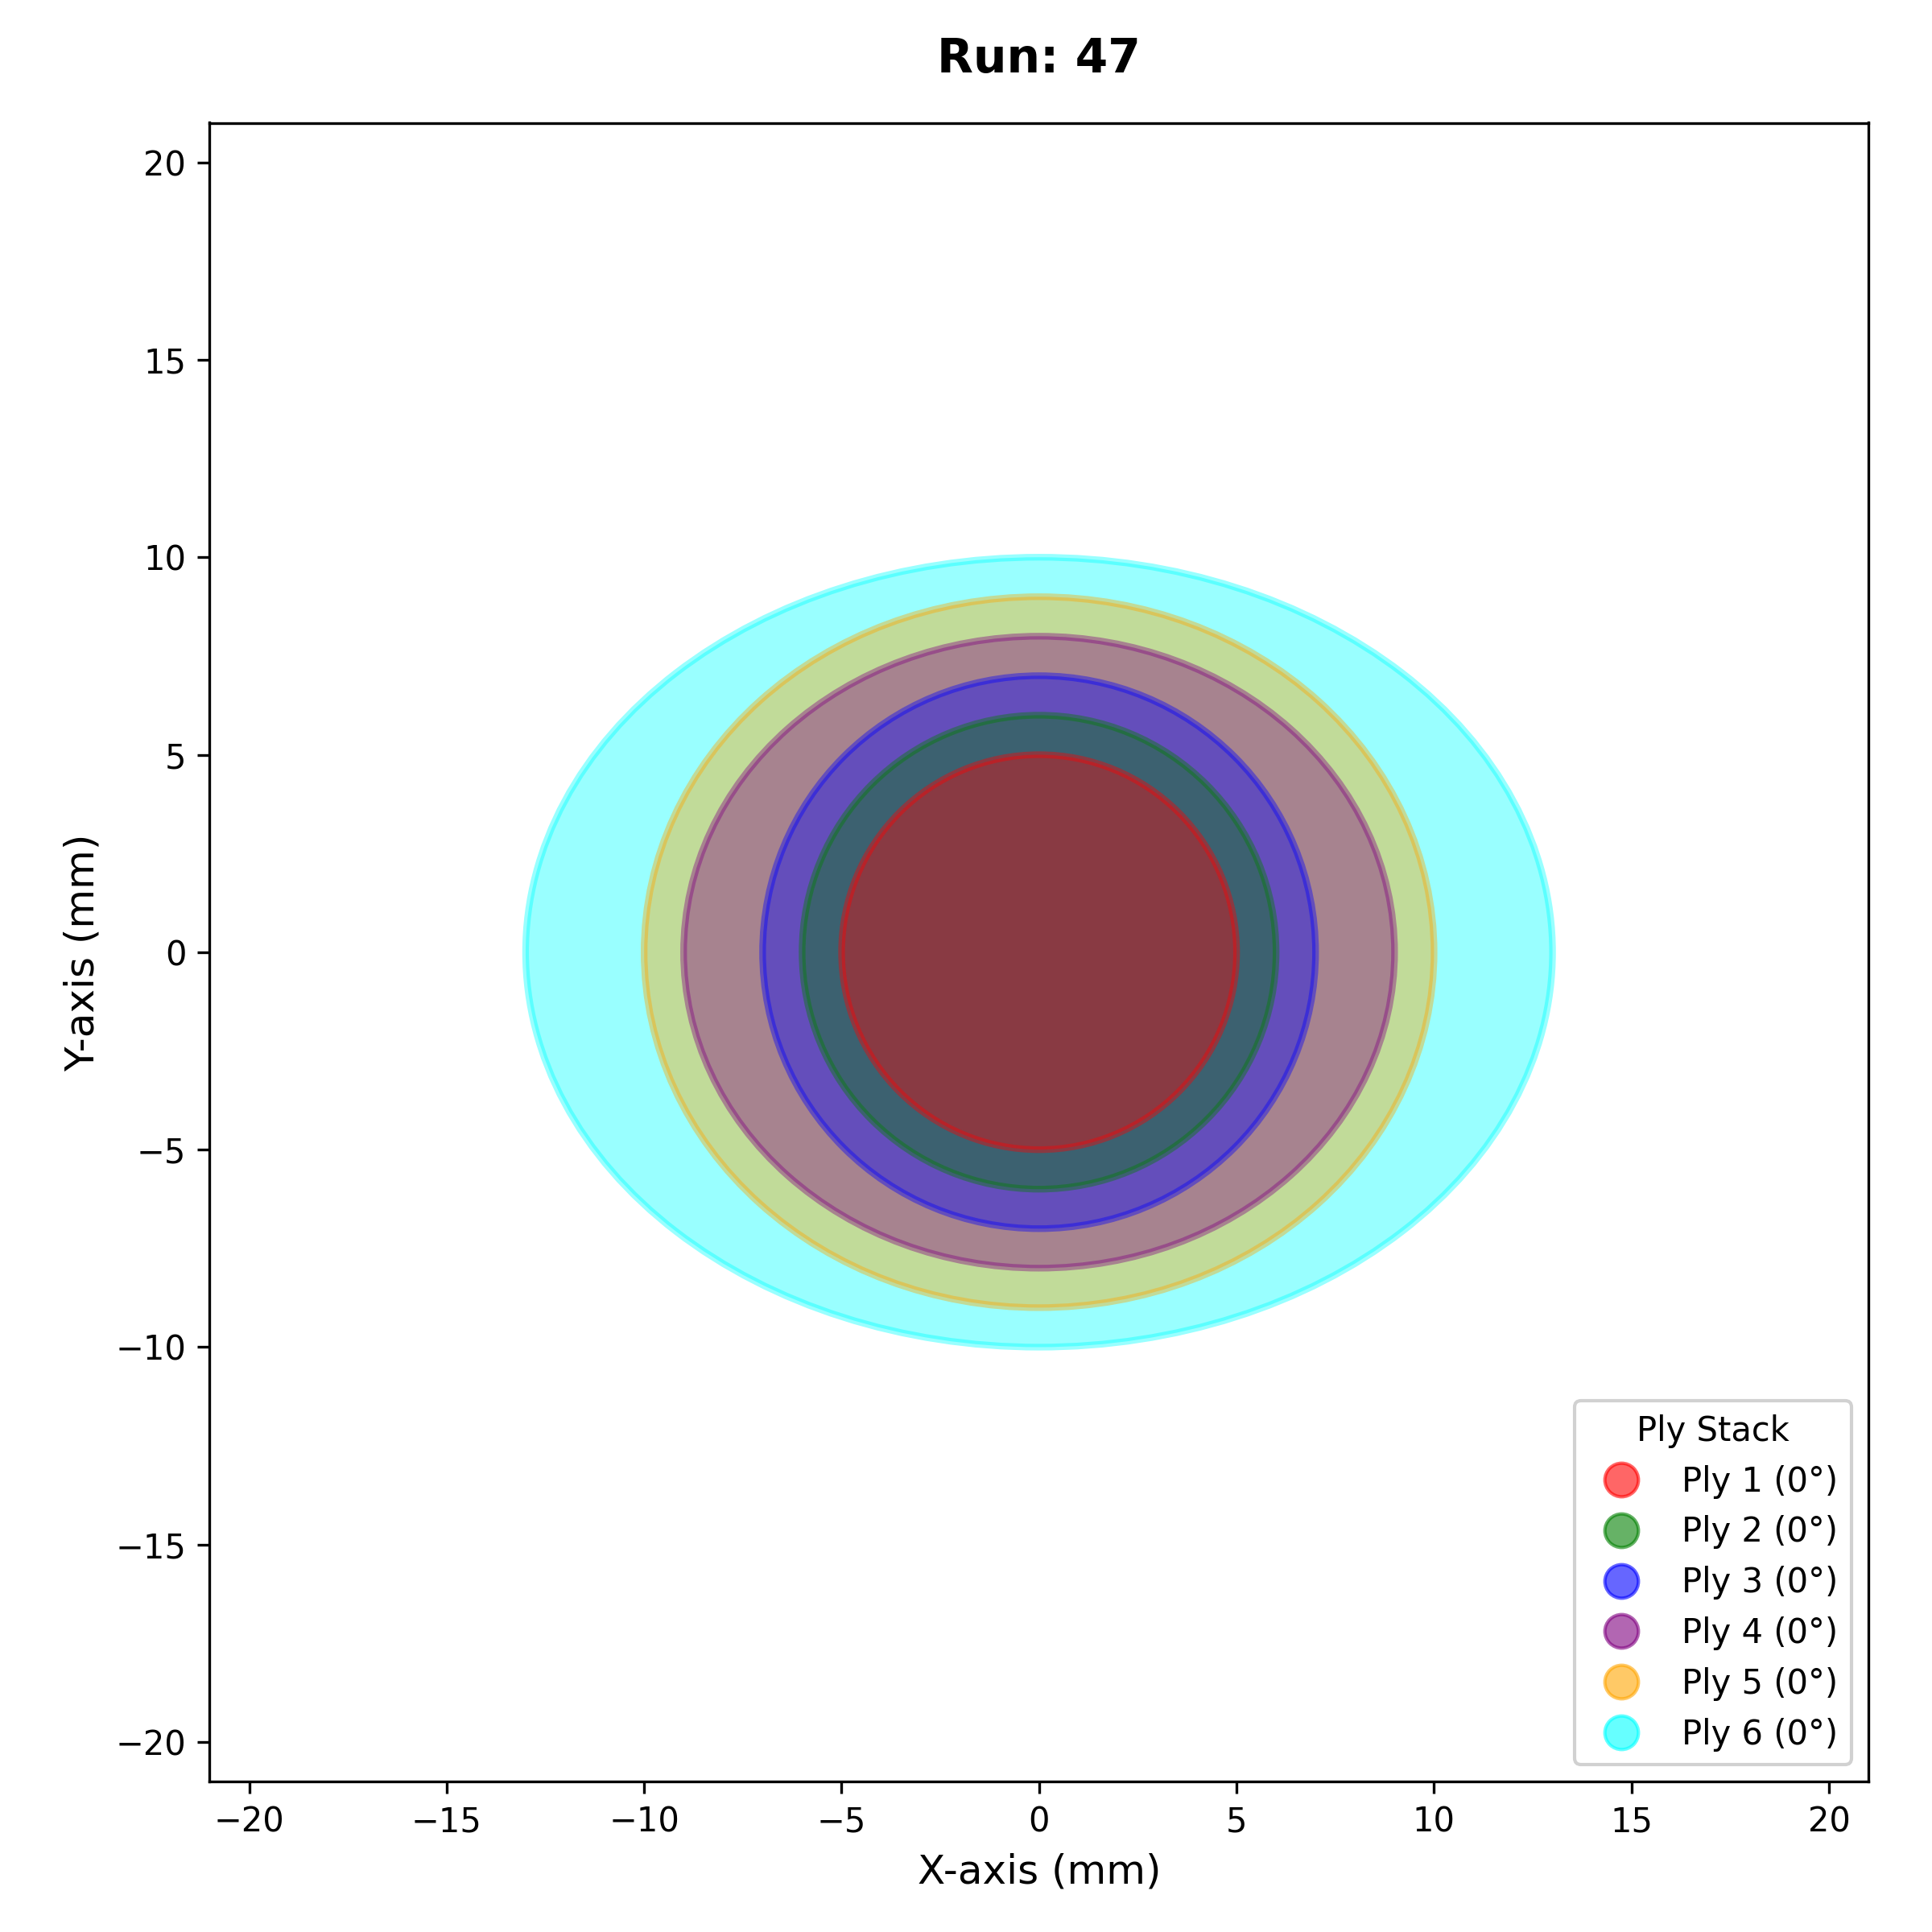
\includegraphics[width=\linewidth]{top_view_Cat0.0_Row2.png}
        \caption{Run 47}
        \label{fig:cat0_run47}
    \end{subfigure}
    \hfill
    \begin{subfigure}[b]{0.48\textwidth}
        \centering
        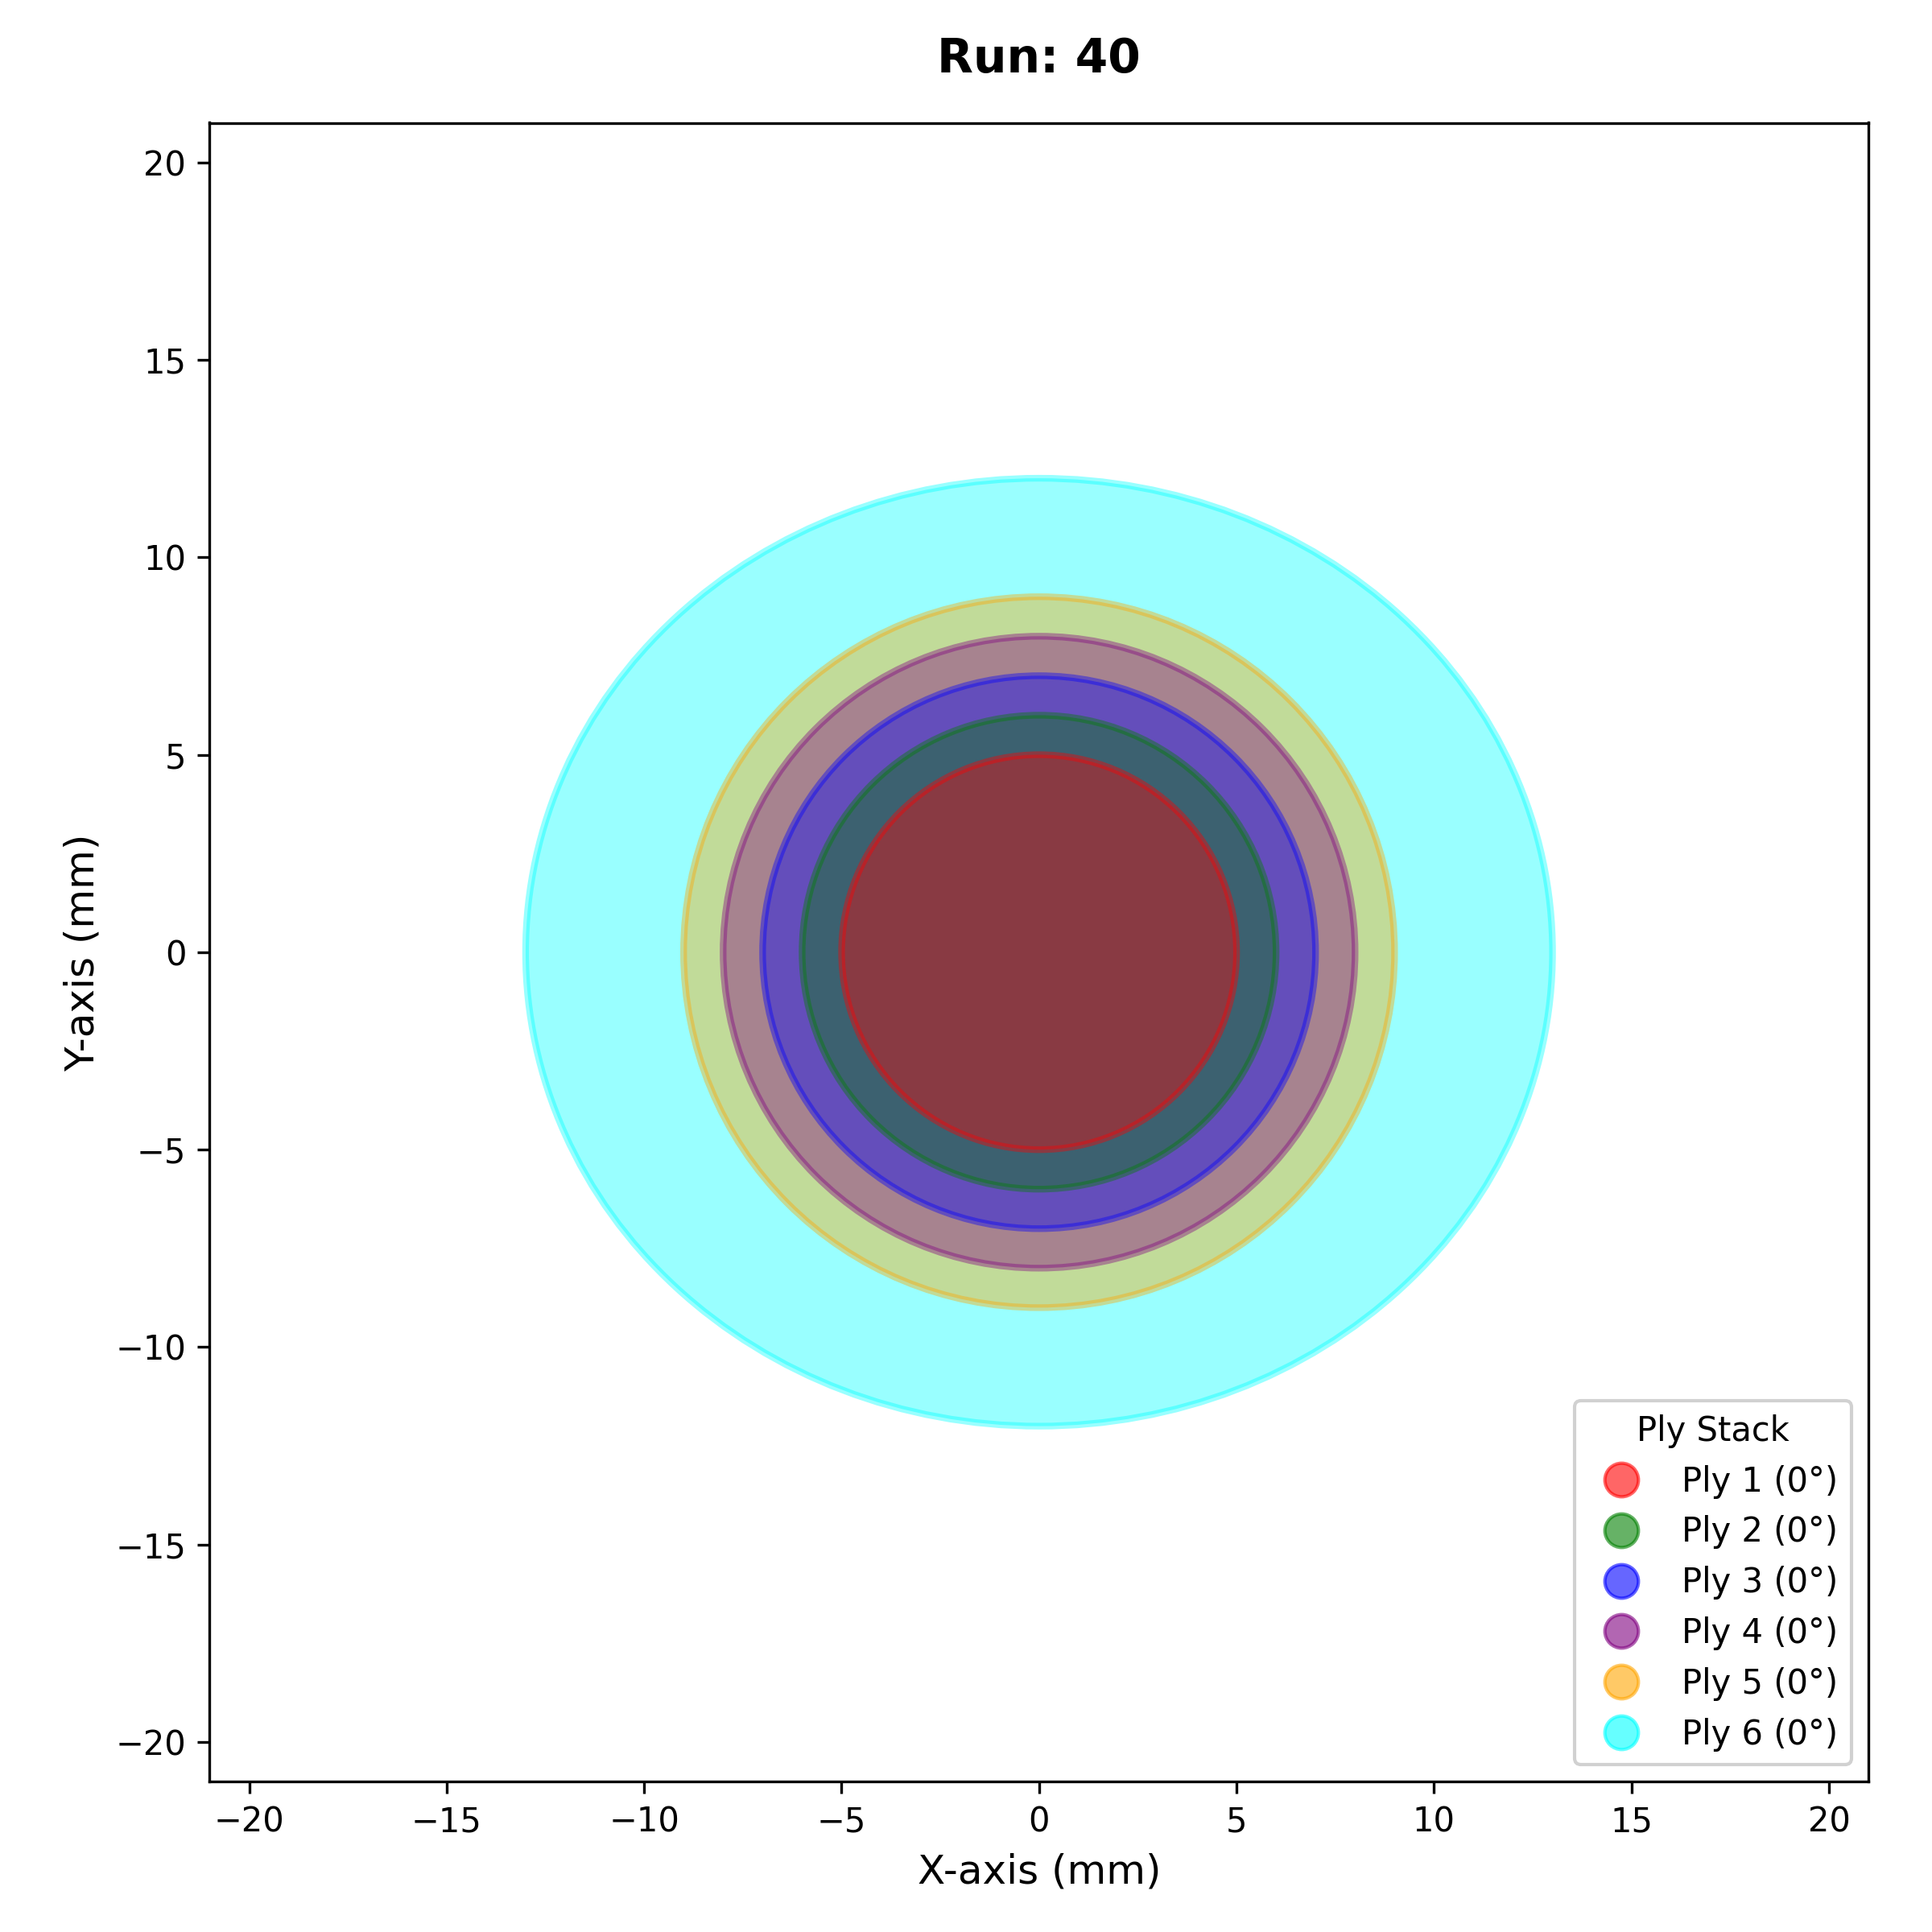
\includegraphics[width=\linewidth]{top_view_Cat0.0_Row3.png}
        \caption{Run 40}
        \label{fig:cat0_run40}
    \end{subfigure}
    
    \caption{\textbf{Morphology of Category 0 Candidates.} The top performers in Category 0 exhibit a highly consistent, circular morphology. The optimization drove the design toward compact, concentric ring structures with minimal gaps, resulting in \new{high strength-to-volume ratio}.}
    \label{fig:cat0_morphology}
\end{figure}

% --- FIGURE 4: CATEGORY 1 TOP CANDIDATES (GEOMETRY) ---
\begin{figure}[htbp]
    \centering
    % Row 1
    \begin{subfigure}[b]{0.48\textwidth}
        \centering
        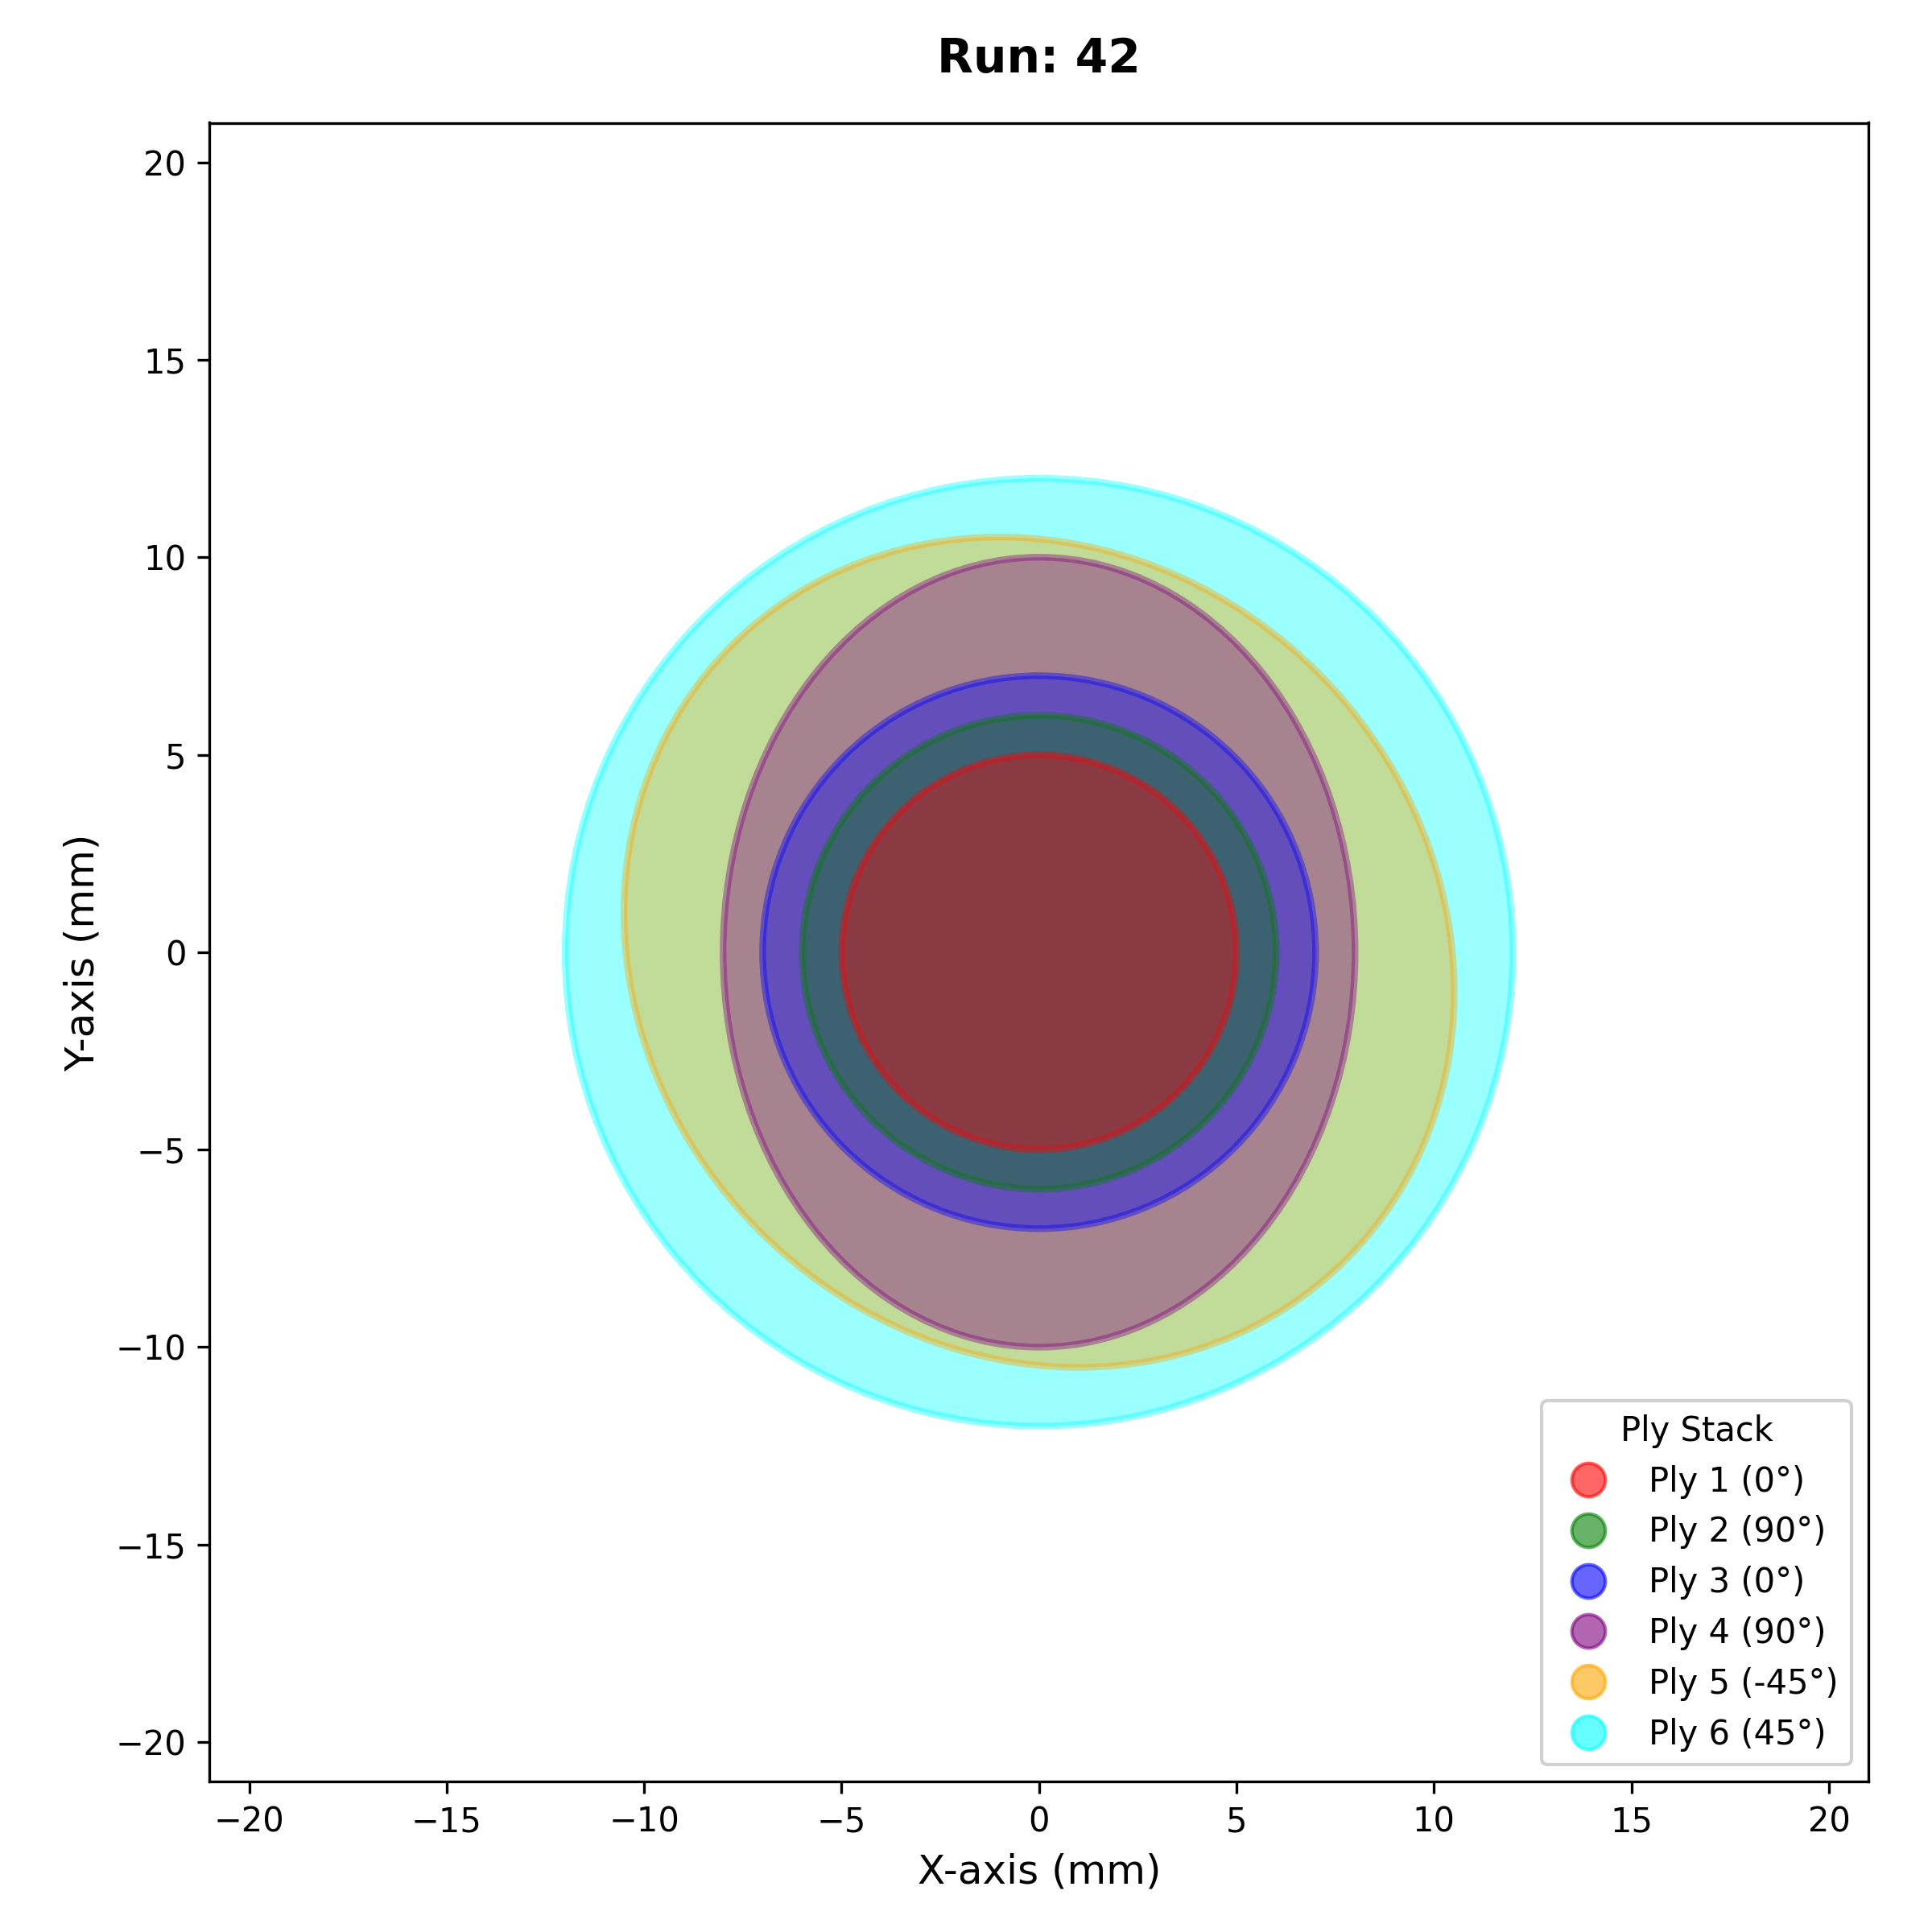
\includegraphics[width=\linewidth]{top_view_Cat1.0_Row0.png}
        \caption{Best Candidate: Run 42}
        \label{fig:cat1_best}
    \end{subfigure}
    \hfill
    \begin{subfigure}[b]{0.48\textwidth}
        \centering
        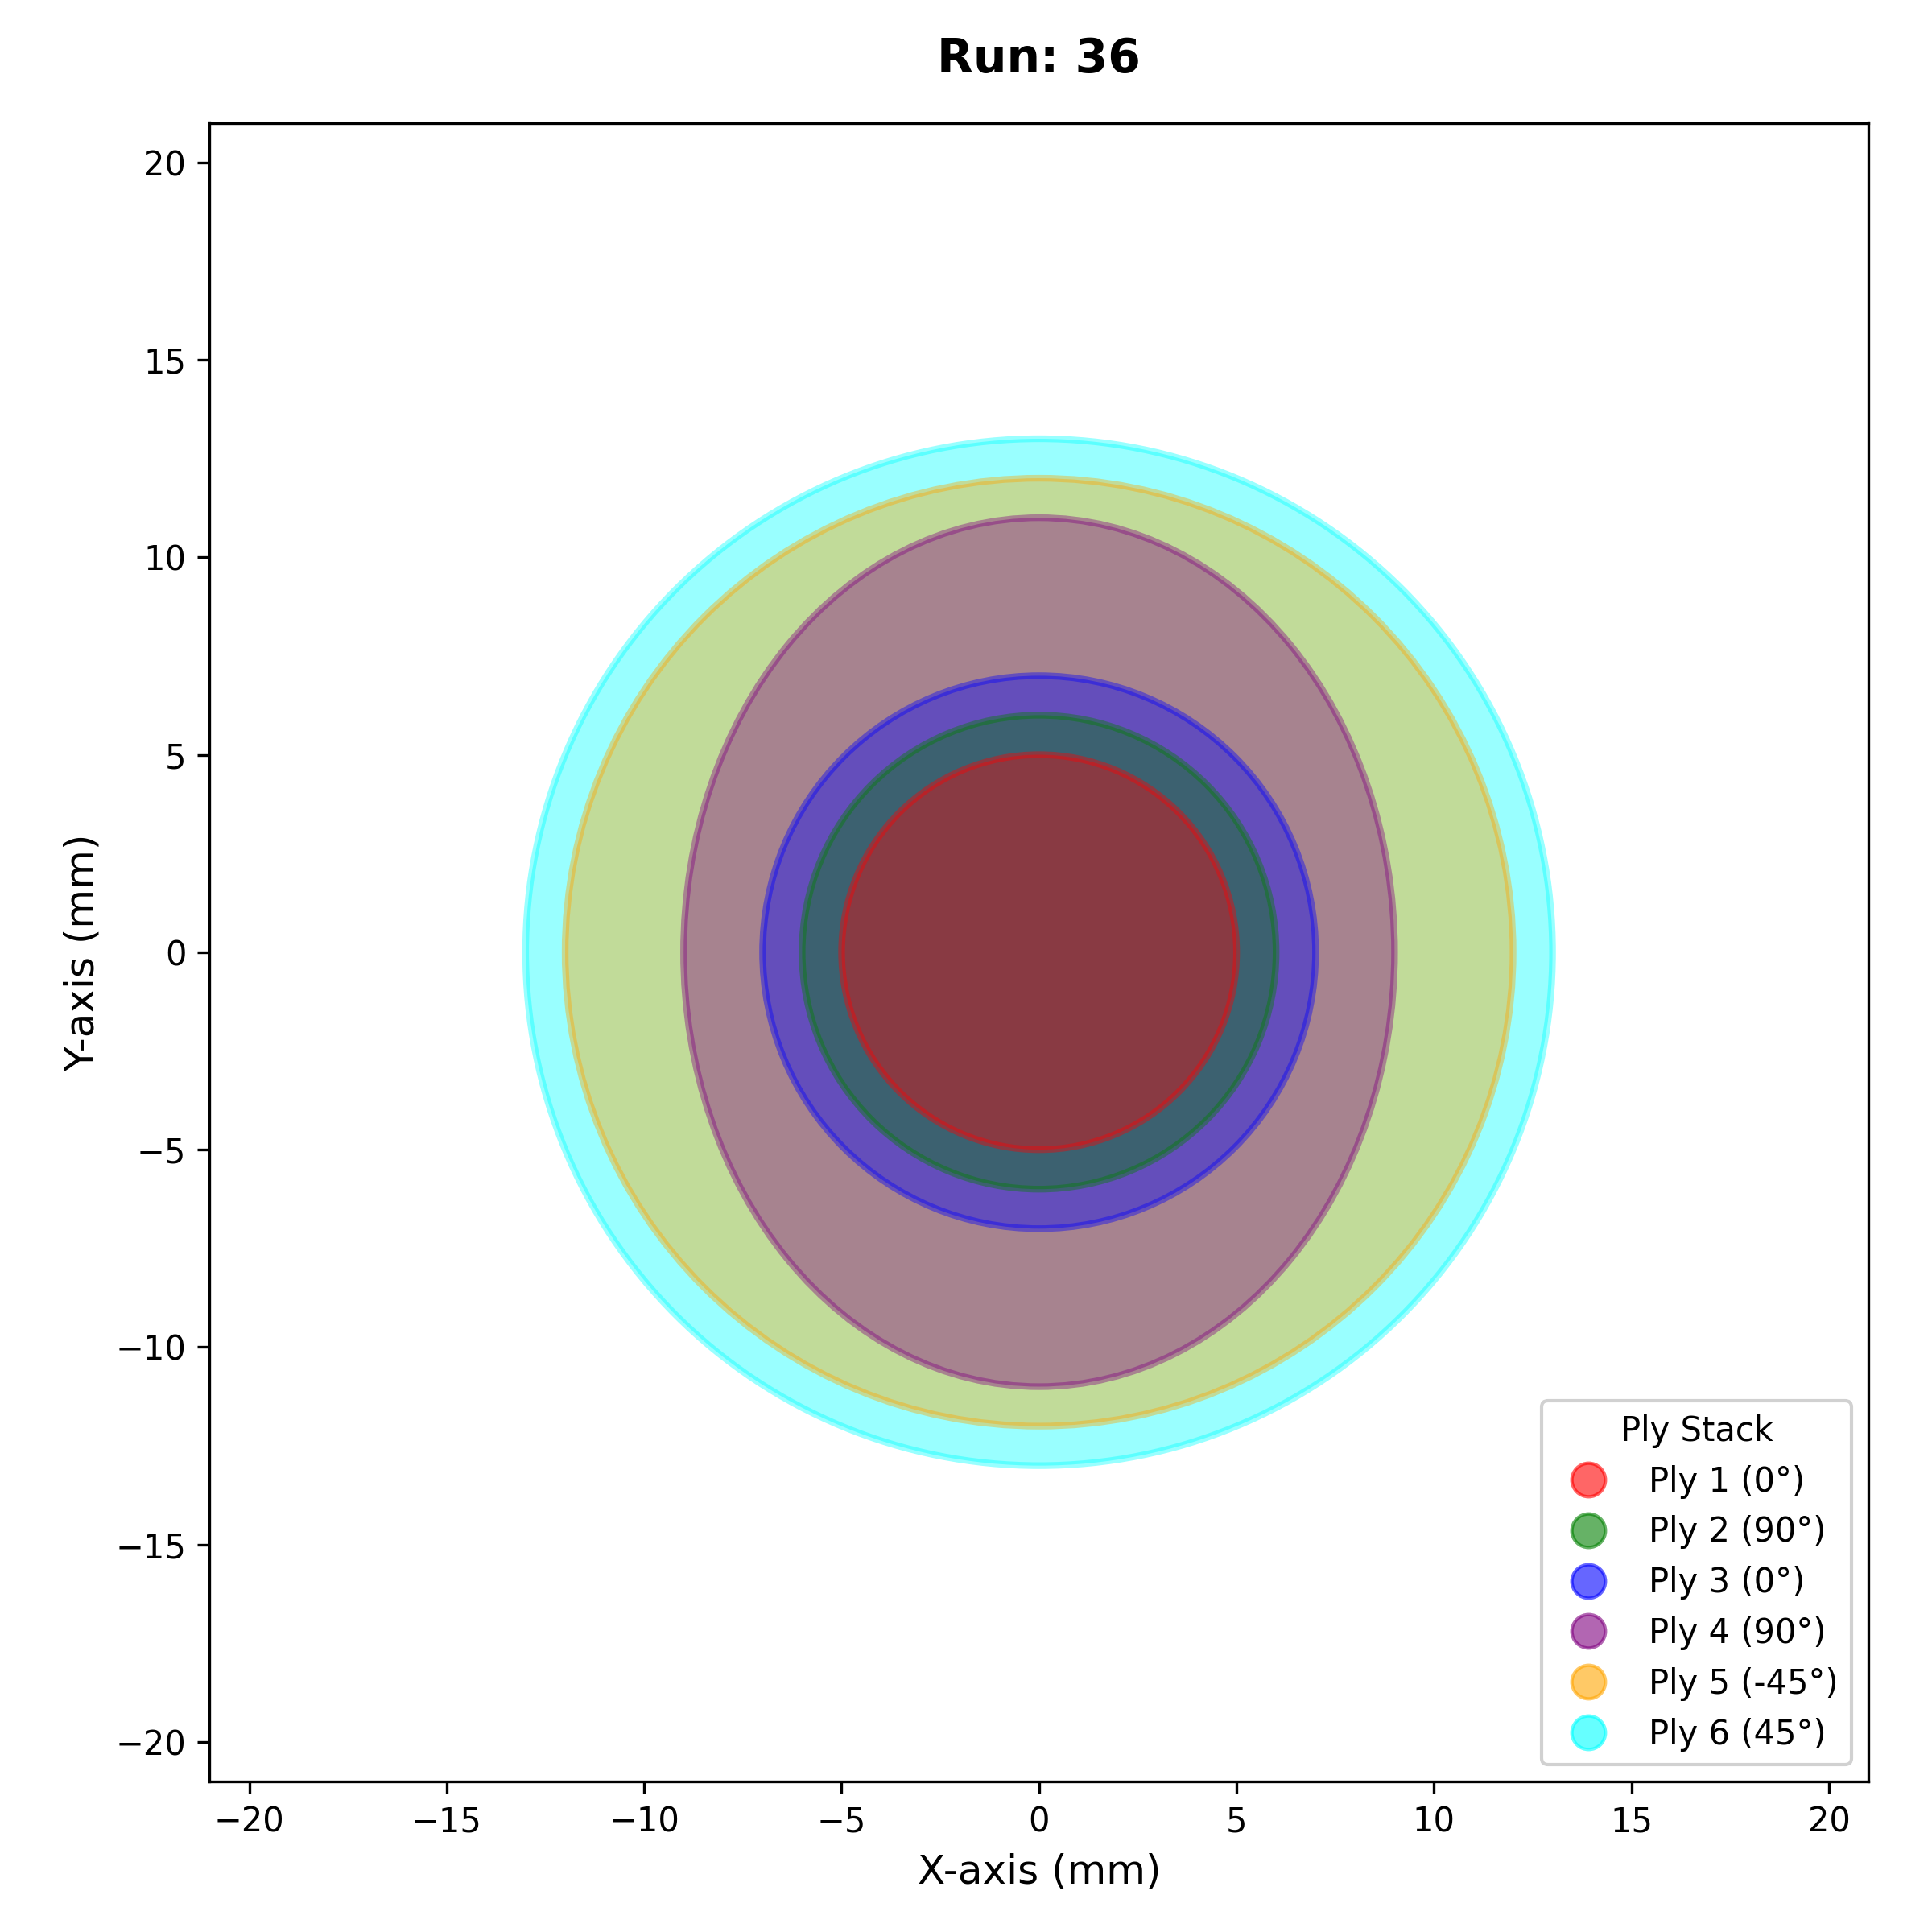
\includegraphics[width=\linewidth]{top_view_Cat1.0_Row1.png}
        \caption{Run 36}
        \label{fig:cat1_run36}
    \end{subfigure}
    
    \par\vspace{0.5cm} % Vertical spacing
    
    % Row 2
    \begin{subfigure}[b]{0.48\textwidth}
        \centering
        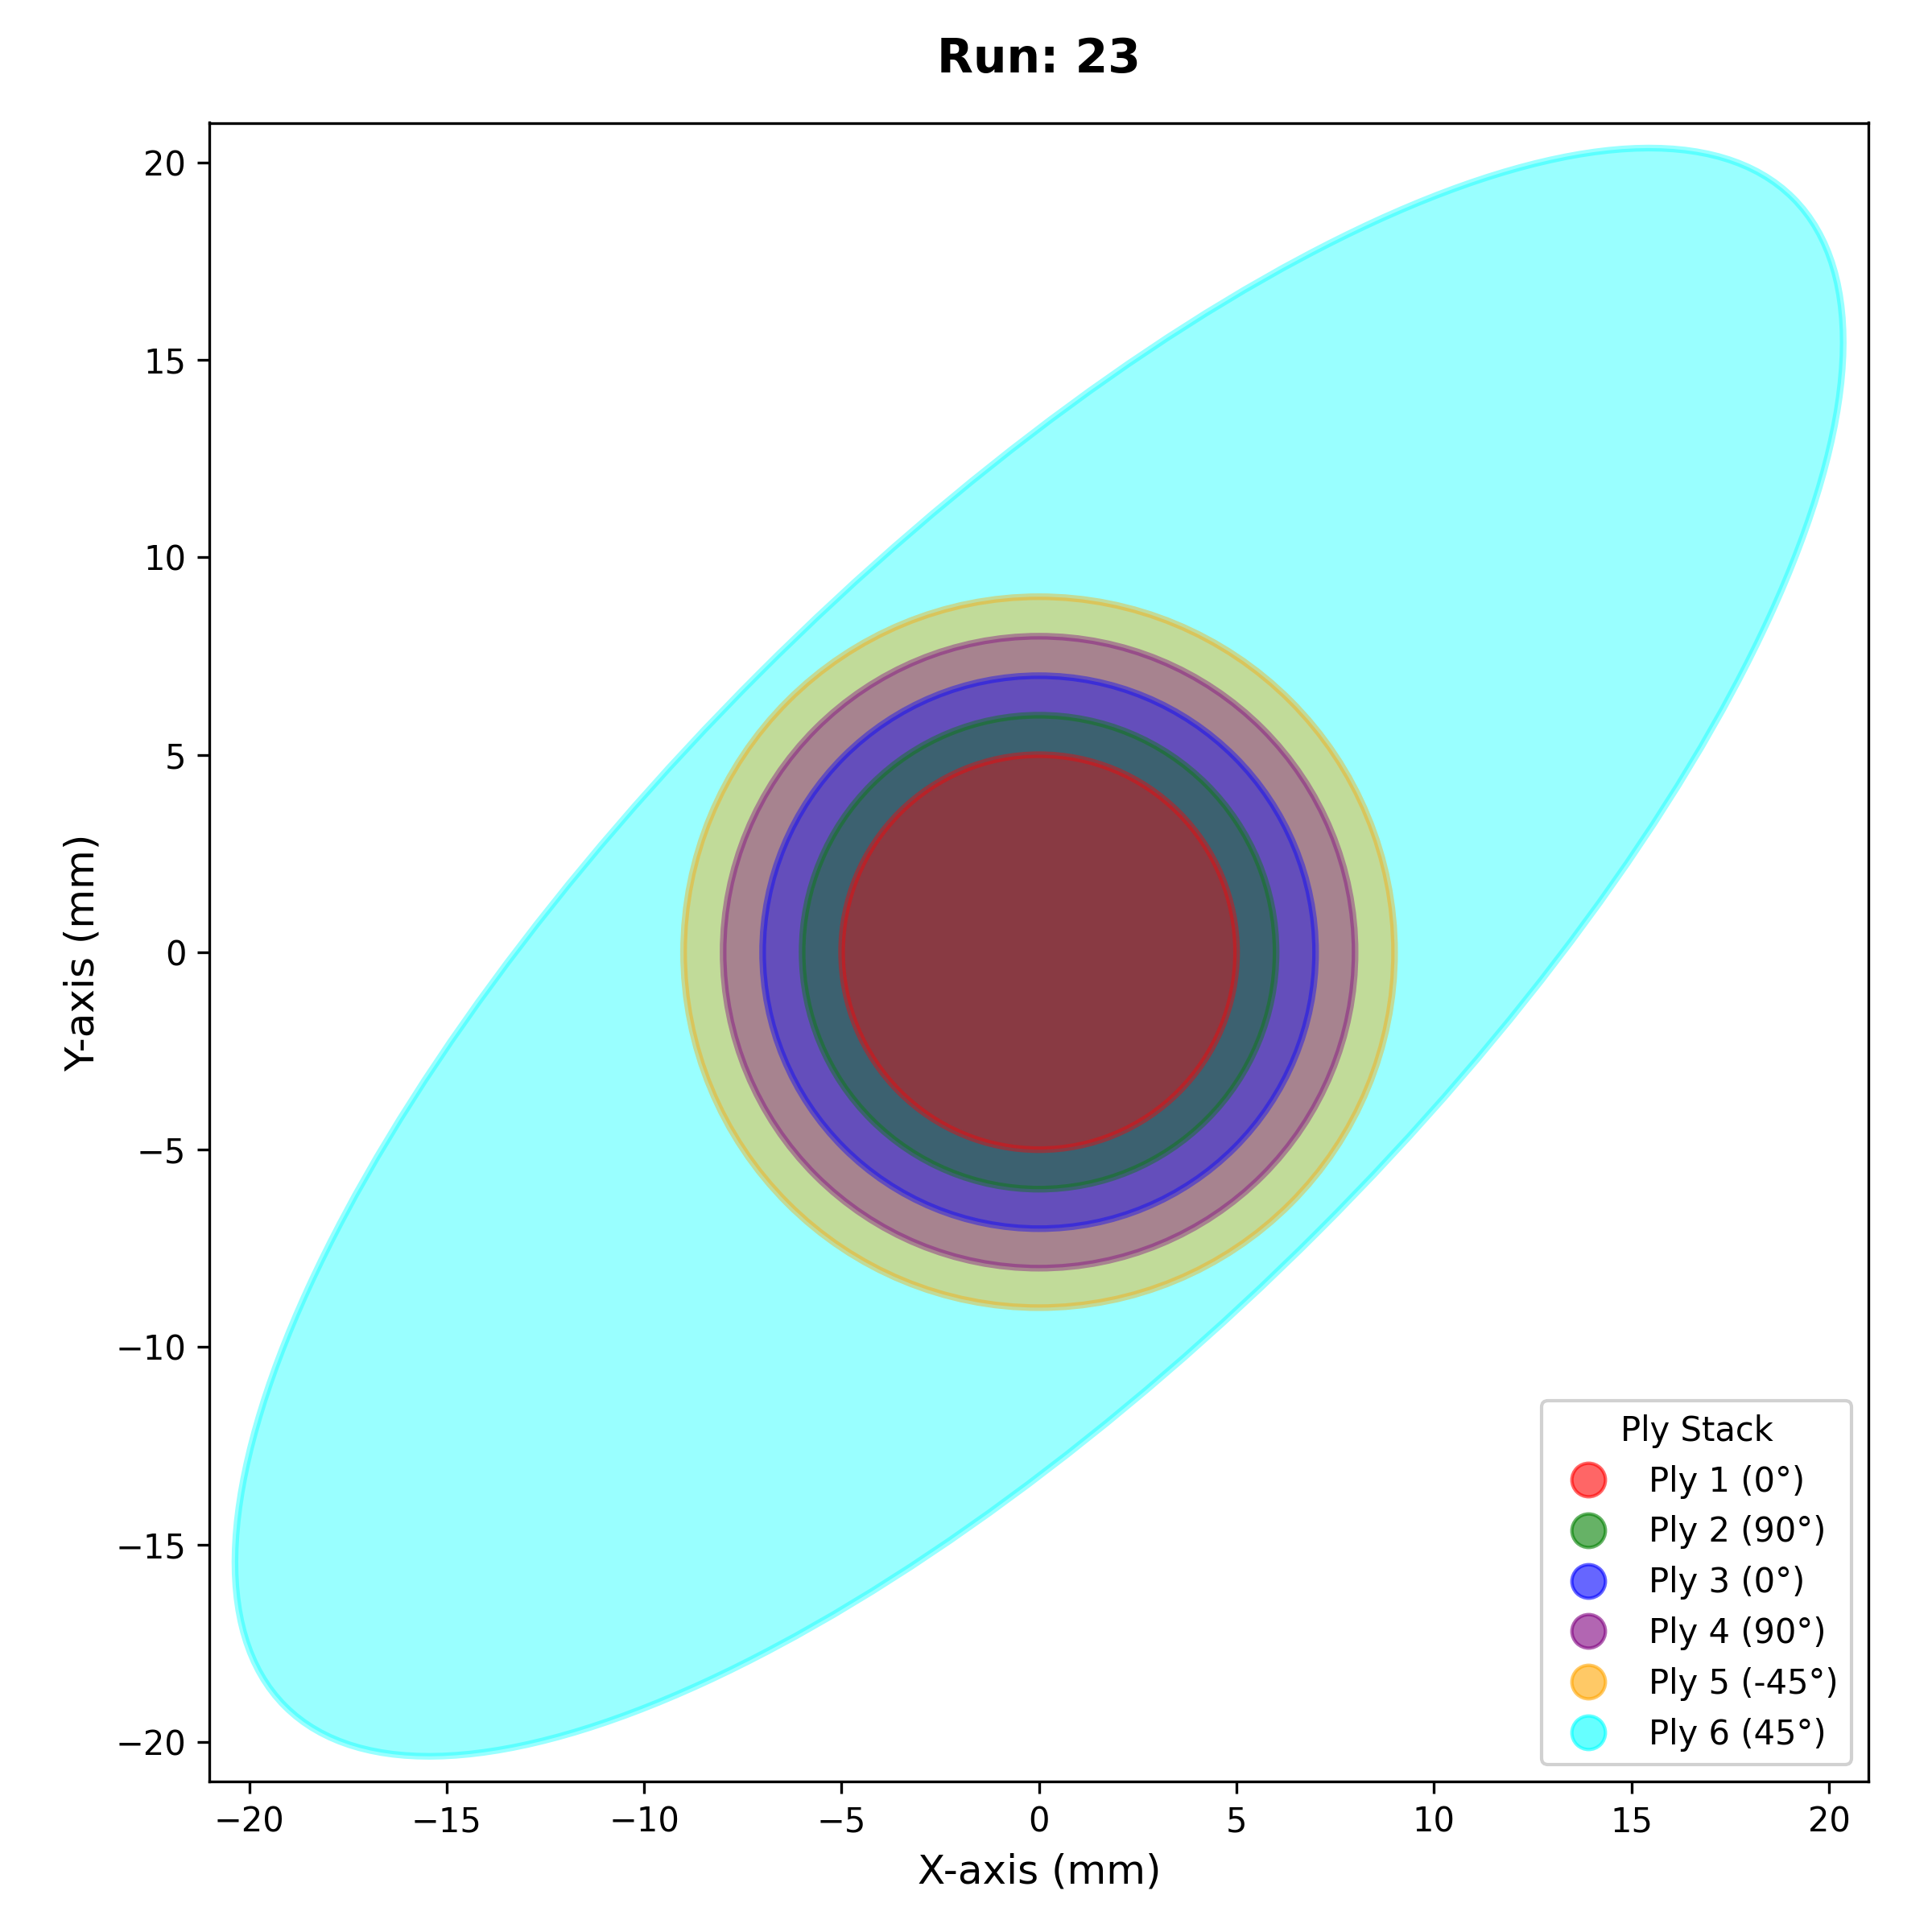
\includegraphics[width=\linewidth]{top_view_Cat1.0_Row2.png}
        \caption{Run 23}
        \label{fig:cat1_run23}
    \end{subfigure}
    \hfill
    \begin{subfigure}[b]{0.48\textwidth}
        \centering
        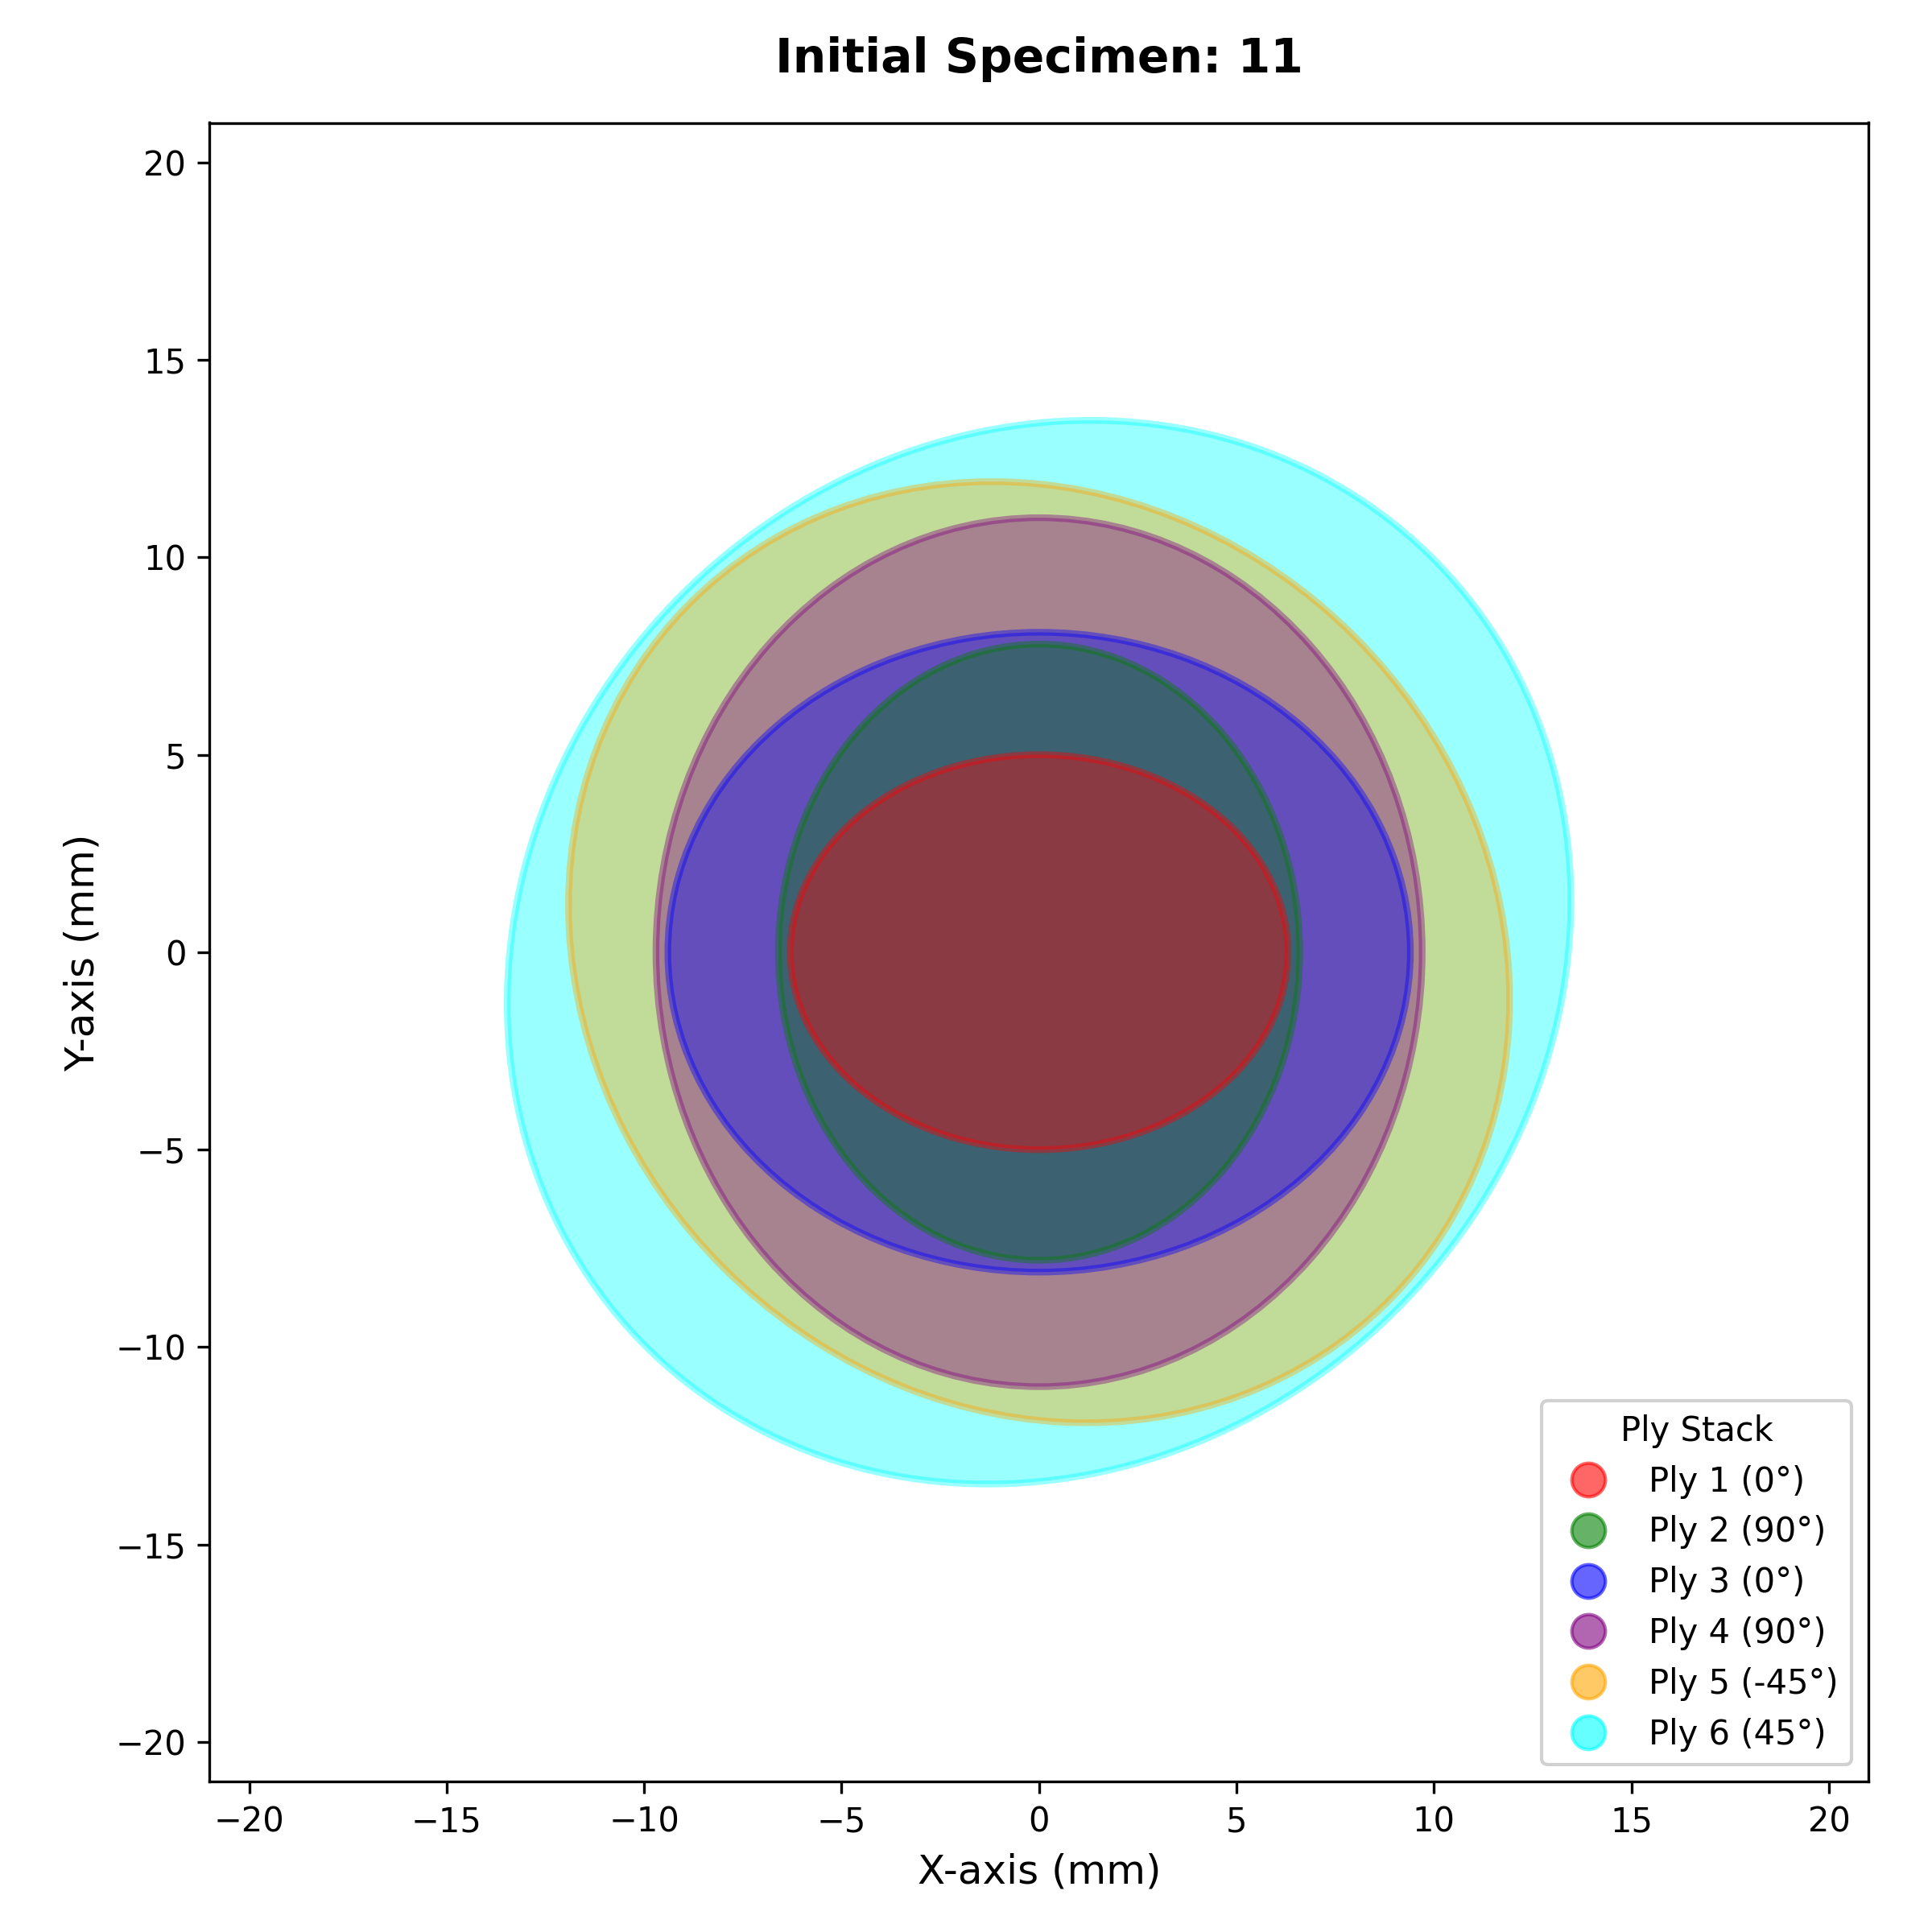
\includegraphics[width=\linewidth]{top_view_Cat1.0_Row3.png}
        \caption{Initial Specimen 9}
        \label{fig:cat1_initial}
    \end{subfigure}
    
    \caption{\textbf{Morphology of Category 1 Candidates.} In contrast to Category 0, these candidates display significant geometric variation, including pronounced elliptical shapes (c) and larger outer dimensions (d). This morphological instability contributed to the slower convergence and lower efficiency ratio.}
    \label{fig:cat1_morphology}
\end{figure}


\subsection{Geometric Morphology of Top Candidates}

Figures \ref{fig:cat0_morphology} and \ref{fig:cat1_morphology} illustrate the physical patch geometries of the top four candidates for each category. These visual results corroborate the efficiency findings discussed previously.

In \textbf{Category 0} (Figure \ref{fig:cat0_morphology}), the candidates share a uniform, compact circular design. The best candidate, Specimen 47 (Fig. \ref{fig:cat0_morphology}a), features tight \new{patch ply} spacing and a reduced overall footprint. The similarity between the initial seed (Specimen 16) and the final optimized runs suggests that the algorithm focused on fine-tuning dimensions rather than radically altering the shape.

\textbf{Category 1} (Figure \ref{fig:cat1_morphology}) reveals a much more chaotic design space. The candidates exhibit visible deviations in aspect ratio, such as the strongly elliptical shape of Run 23 (Fig. \ref{fig:cat1_morphology}c) and the expansive outer rings of Initial Specimen 9 (Fig. \ref{fig:cat1_morphology}d). While the best candidate (Run 42, Fig. \ref{fig:cat1_morphology}a) managed to recover a circular form similar to Category 0, the presence of these irregular geometric variations throughout the search history explains the model's difficulty in converging and the resulting "volume bloat" observed in the data.

\subsection{Limitations of the Study}
\label{sec:limitations}

While the proposed framework demonstrates significant \new{computational efficiency} gains, several limitations should be considered when interpreting the results:

\begin{enumerate}
    \item \textbf{Idealized Numerical Baseline:} The training data was generated using high-fidelity FEM that assumes "perfect" manufacturing. The simulations model the adhesive interface with uniform thickness and properties, neglecting process-induced defects such as porosity, variable bond-line thickness, or heat-affected zones (HAZ) from the laser ablation. Consequently, the "Optimal" 71.2 kN strength represents a theoretical upper bound; experimental values may exhibit higher variance.
    
    \item \textbf{Single Loading Condition:} The optimization was strictly targeted at \textit{Static Compressive Strength} (UCS). While compression is the critical design driver for stepped repairs, the optimized geometries have not been validated under tensile, bending, or fatigue loading. A design that maximizes buckling and debonding resistance (e.g., compact footprint) might be suboptimal for fatigue crack propagation, where larger bond areas are typically preferred.
    
    \item \textbf{Material Specificity:} The Deep Kernel was trained on a specific aerospace-grade material system (IMS 24K 977-2) and a specific stacking sequence. While the \textit{methodology} is universal, the \textit{learned geometric rules} (e.g., the specific aspect ratios identified for Category 1) are likely material-dependent. Applying this \new{framework} to a different layup or resin system would require re-training, although Transfer Learning could significantly accelerate this process.
\end{enumerate}



% ==============================================================================
% 5. CONCLUSIONS
% ==============================================================================
\section{Conclusions}
\label{sec:conclusion}

This study presented a probabilistic active learning framework for the automated optimization of stepped composite repairs. By coupling a high-fidelity Finite Element baseline with a Deep Kernel Gaussian Process (DKGP), the framework successfully \new{solved the constrained optimization problem}, identifying optimal repair geometries under strict manufacturing constraints without relying on computationally prohibitive brute-force sampling.

The following key conclusions are drawn:
\begin{enumerate}
    \item \textbf{Computational Efficiency:} The \new{Deep Kernel Active Learning (DKAL) framework} demonstrated a 96\% reduction in computational cost compared to theoretical evolutionary baselines (Genetic Algorithms). The framework identified the global optimum in just \textbf{59 evaluations} for standard laminates (Category 0) and \textbf{92 evaluations} for complex off-axis configurations (Category 1), effectively replacing thousands of explicit FEM simulations with a query-efficient surrogate.
    
    \item \textbf{Physics-Aware Learning:} The \new{framework} exhibited distinct learning behaviors driven by the underlying mechanics. For standard repairs, it rapidly identified the \new{strength-recovery limit} ($\approx 95\%$ of parent strength). For complex repairs, it autonomously detected—and eventually learned to avoid—non-linear bifurcation modes, specifically the premature debonding caused by aggressive \new{patch-ply} step increments.
    
    \item \textbf{Geometric Design Rules:} The optimization results challenge standard "constant overlap" repair guidelines. The AI-derived optimal shapes suggest that for compressive loading, \new{the strength-to-volume ratio} is maximized by tuning the step gradients to be gradual in the load-bearing direction while keeping the transverse footprint compact. In Category 1, avoiding large step jumps between off-axis \new{patch plies} proved critical to preventing premature instability.
    
    \item \textbf{Architectural Robustness:} The proposed "Two-Stage" adaptive strategy—transitioning from a shallow RBF network for exploration to a Deep Matern network for exploitation—was essential. The ablation study confirmed that the Matern kernel's capacity to model non-smooth transitions was required to capture the sudden strength drops associated with adhesive debonding, which standard smooth kernels failed to resolve.
\end{enumerate}

The immediate next step for this research involves the physical manufacturing and testing of the identified optimal candidates (Run 8 and Run 42) using an automated laser repair cell. This validation will assess the predictive accuracy of the framework against real-world experimental scatter. Furthermore, to address process variabilities such as heat-affected zones or depth tolerances, future iterations will incorporate "Input Uncertainty" into the Gaussian Process, guiding the \new{optimization} toward robust optima that remain high-performing even under manufacturing deviations.

From a methodological perspective, a promising direction is the transition to a hybrid, \textit{Physics-Informed} framework. By embedding analytical closed-form expressions for adhesive bond strength \cite{psarras2024design} directly into the Deep Kernel's loss function, we anticipate a further reduction in dataset requirements by 30--50\%, as the model would no longer need to learn basic mechanical correlations purely from data. Finally, to generalize the approach across different stacking sequences, \textit{Transfer Learning} techniques will be explored, utilizing a pre-trained "Universal" Deep Kernel to warm-start optimization for new repair scenarios, potentially reducing the exploration phase to fewer than 10 iterations.


% ==============================================================================
% BACK MATTER
% ==============================================================================



\section*{Declaration of Competing Interest}
The authors declare that they have no known competing financial interests or personal relationships that could have appeared to influence the work reported in this paper.

\section*{Data Availability}
The raw data supporting the findings of this study (specifically the high-fidelity FEM input decks and detailed output databases) are available from the corresponding author on reasonable request. 

The complete source code for the Deep Kernel Active Learning framework, including the surrogate model architecture and the Bayesian optimization pipeline, is openly available in the public GitHub repository: \url{https://github.com/johnstamly/Active_learning_pipeline}.

\section*{Acknowledgments}
This work was supported by the Thick Composite Repairs Project, a collaboration between University of Patras and Naval Group.

\section*{Declaration of generative AI and AI-assisted technologies in the manuscript preparation process}

During the preparation of this work the author(s) used Google Gemini 3.0 Pro in order to refine the English language, improve readability, and assist with LaTeX formatting. After using this tool/service, the author(s) reviewed and edited the content as needed and take(s) full responsibility for the content of the published article.

% ==============================================================================
% CRediT authorship contribution statement
% ==============================================================================
\section*{CRediT authorship contribution statement}
\textbf{Giannis Stamatelatos:} Methodology, Software, Investigation, Data Curation, Writing - Original Draft.
\textbf{Emilien Billaudeau:} Resources, Investigation.
\textbf{Maëlle Sergolle:} Investigation.
\textbf{Thomas Balutch:} FEM Software.
\textbf{Vassilis Kostopoulos:} Resources, Project Administration, Funding Acquisition.
\textbf{Theodoros Loutas:} Methodology, Supervision, Writing - Review \& Editing.
\textbf{Spyridon Psarras:} Conceptualization, Methodology, Formal Analysis, Supervision, Writing - Review \& Editing, Resources, Project Administration.

% ==============================================================================
% REFERENCES
% ==============================================================================
\bibliography{../references}

\end{document}